\documentclass[12pt,a4paper]{report}

%==============================================================================
% PREAMBLE AND PACKAGES (Aligned with CEK / KTU B.Tech Project Format)
%==============================================================================
\usepackage{graphicx}
\usepackage{amsmath}
\usepackage{fancyhdr}
\usepackage{cite}
\usepackage{a4wide}
\usepackage{float}
\usepackage{epsfig}
\usepackage{longtable}
\usepackage{enumerate}
\usepackage{afterpage}
\usepackage{multirow}
\usepackage{ragged2e}
\usepackage{gensymb}
\usepackage{amsfonts} 
\usepackage{amssymb}
\usepackage[left=3.5cm,top=1.5cm,right=3cm,bottom=3cm]{geometry}
\usepackage{setspace}           
\usepackage{txfonts}
\usepackage{standalone}
\usepackage{tikz}
\usepackage{fontawesome5}
\usetikzlibrary{calc, shapes.geometric, arrows, arrows.meta, positioning, fit, backgrounds, shadows, tikzmark}

% Color definitions for TikZ diagrams
\definecolor{lavenderDark}{RGB}{15, 44, 89}
\definecolor{lavenderDeep}{RGB}{10, 28, 58}
\definecolor{lavenderMedium}{RGB}{29, 78, 158}
\definecolor{lavenderLight}{RGB}{240, 246, 255}
\definecolor{lavenderBorder}{RGB}{180, 205, 237}
\definecolor{lavenderAccent}{RGB}{2, 132, 199}
\definecolor{prismNavy}{RGB}{15, 44, 89}
\definecolor{prismBlue}{RGB}{29, 78, 158}
\definecolor{prismTeal}{RGB}{13, 148, 136}
\definecolor{prismMint}{RGB}{236, 253, 245}
\definecolor{prismGold}{RGB}{217, 119, 6}
\definecolor{prismDark}{RGB}{15, 23, 42}
\definecolor{prismLight}{RGB}{248, 250, 252}
\definecolor{prismIndigo}{RGB}{30, 58, 138}
\definecolor{prismSlate}{RGB}{100, 116, 139}
\definecolor{statusFail}{RGB}{220, 38, 38}
\definecolor{cInput}{RGB}{241, 245, 249}
\definecolor{cStem}{RGB}{224, 242, 254}
\definecolor{cStage1}{RGB}{209, 250, 229}
\definecolor{cStage2}{RGB}{254, 243, 199}
\definecolor{cStage3}{RGB}{254, 226, 226}
\definecolor{cStage4}{RGB}{207, 250, 254}
\definecolor{cHead}{RGB}{219, 234, 254}
\definecolor{cOutput}{RGB}{255, 228, 230}
\definecolor{cDeliverable}{RGB}{204, 251, 241}

\usepackage{subfiles}
\usepackage{adjustbox}
\usepackage{tcolorbox}
\tcbuselibrary{skins}

\newcommand{\Usefont}[1]{\fontfamily{#1}\selectfont}

\usepackage{lscape}
\linespread{1.5}

\usepackage{url}
\usepackage{subcaption}
\usepackage[intoc, english]{nomencl}
\usepackage[nottoc]{tocbibind}
\usepackage{booktabs}
\usepackage{array}
\usepackage{tabularx}
\usepackage{xltabular}
\usepackage{hyperref}

\hypersetup{
    plainpages=false,
    pdfpagelabels=true,
    colorlinks=true,
    linkcolor=black,
    citecolor=black,
    urlcolor=black,
    pdftitle={Explainable AI for Multivariate Time Series Pattern Exploration: Latent Space Visual Analytics With Temporal Fusion Transformer and Variational Autoencoders in Power Grid Event Diagnosis},
    pdfauthor={Adwaith K Rajeesh, Anamika P, Georgy Binu George, Inshad Ibrahim C}
}

% Spacing and line-breaking settings to prevent overflow and overfull hboxes
\setlength{\headheight}{15pt}
\hyphenpenalty=1000
\tolerance=2000
\emergencystretch=2.5em

\bibliographystyle{IEEEtran}
\renewcommand{\bibname}{References}

% Figure search path
\graphicspath{{figures/}{diagrams/}{./}}

%==============================================================================
% METADATA DEFINITIONS (Project Group & CEK)
%==============================================================================
\gdef \title{EXPLAINABLE AI FOR MULTIVARIATE TIME SERIES PATTERN EXPLORATION: LATENT SPACE VISUAL ANALYTICS WITH TEMPORAL FUSION TRANSFORMER AND VARIATIONAL AUTOENCODERS IN POWER GRID EVENT DIAGNOSIS}
\gdef \shorttitle{Explainable AI for Multivariate Time Series Pattern Exploration}

\gdef \authorA{ADWAITH K RAJEESH}
\gdef \rollnoA{KNP23CS018}

\gdef \authorB{ANAMIKA P}
\gdef \rollnoB{KNP23CS029}

\gdef \authorC{GEORGY BINU GEORGE}
\gdef \rollnoC{KNP23CS048}

\gdef \authorD{INSHAD IBRAHIM C}
\gdef \rollnoD{KNP23CS055}

\gdef \acadyear{2026--2027}
\gdef \submonth{October 2026}
\gdef \month{October 2026}
\gdef \date{27-10-2026}
\gdef \dept{Computer Science and Engineering}
\gdef \deptabbr{Dept.\ of CSE}
\gdef \degree{Bachelor of Technology}
\gdef \branch{Computer Science and Engineering}
\gdef \college{College of Engineering Karunagappally}
\gdef \collegeplace{Kollam}
\gdef \collegetown{Karunagappally}

\gdef \guide{Ms. Ansiya Mohammed Ali}
\gdef \guidedes{Assistant Professor}
\gdef \coordinator{Dr. Smitha}
\gdef \coordinatordes{Associate Professor and HOD}
\gdef \semcordinatorA{Dr. Smitha}
\gdef \semcordinatorAdes{Associate Professor and HOD}
\gdef \hod{Dr. Smitha}
\gdef \hoddes{Associate Professor and HOD}

\ifdefined\candidateName
  \newcommand{\isIndividualReport}{true}
\fi
\providecommand{\candidateName}{\authorA}
\providecommand{\candidateRoll}{\rollnoA}

%==============================================================================
% DOCUMENT BODY
%==============================================================================

\begin{document}

%------------------------------------------------------------------------------
% FRONT MATTER
%------------------------------------------------------------------------------
\hypersetup{pageanchor=false}
%==================================coverpage.tex================================

\thispagestyle{empty}
\newgeometry{left=3cm,right=3cm,top=2cm,bottom=2.2cm}
\begin{titlepage}
\subfile{design_cover}
	\begin{center}\fontfamily{ptm}\selectfont
		{\fontsize{13.5}{17.5}\selectfont \bfseries
			EXPLAINABLE AI FOR MULTIVARIATE TIME SERIES\\[4pt]
			PATTERN EXPLORATION: LATENT SPACE VISUAL\\[4pt]
			ANALYTICS WITH TEMPORAL FUSION TRANSFORMER\\[4pt]
			AND VARIATIONAL AUTOENCODERS IN POWER GRID\\[4pt]
			EVENT DIAGNOSIS\par}
		\vspace*{14pt}
		{\large \Usefont{pzc}
			A PROJECT REPORT \par
			\vspace*{4pt}
			Submitted to the APJ Abdul Kalam Technological University \par
			\vspace*{4pt}
			in partial fulfillment of requirements for the award of degree\par}
		\vspace*{8pt}
		{\large \bfseries Bachelor of Technology}\par
		{\normalsize in}\par
		{\large \bfseries \branch}\par
		\vspace*{10pt}
		{\normalsize by}\par
		\vspace*{6pt}
		\begin{tabular}{l@{\hspace{1.5cm}}l}
			\normalsize\bfseries ADWAITH K RAJEESH & \normalsize\bfseries KNP23CS018 \\
			\normalsize\bfseries ANAMIKA P & \normalsize\bfseries KNP23CS029 \\
			\normalsize\bfseries GEORGY BINU GEORGE & \normalsize\bfseries KNP23CS048 \\
			\normalsize\bfseries INSHAD IBRAHIM C & \normalsize\bfseries KNP23CS055
		\end{tabular}\par
		\vspace*{14pt}
		{
\includegraphics[width=3.6cm]{cek-logo.png}}\par
		\vspace{\stretch{1.0}}
		{\small \bfseries DEPARTMENT OF COMPUTER SCIENCE AND ENGINEERING}\par
		\vspace*{4pt}
		{\bfseries COLLEGE OF ENGINEERING KARUNAGAPPALLY}\par
		\vspace*{4pt}
		{\bfseries KOLLAM, KERALA}\par
		\vspace*{4pt}
		{\bfseries \submonth}\par
	\end{center}
\end{titlepage}
\restoregeometry


%=============================vision_mission.tex===============================
\thispagestyle{empty}

\begin{center}
    \vspace*{0.2cm}
    
\includegraphics[width=3.6cm]{cek-logo.png}\par
    \vspace*{0.5cm}
    {\bfseries\large COLLEGE OF ENGINEERING KARUNAGAPPALLY\par}
    \vspace*{0.2cm}
    {\bfseries Thodiyoor -- 690523\par}
    \vspace*{0.2cm}
    {\bfseries\large DEPARTMENT OF COMPUTER SCIENCE AND ENGINEERING\par}
    
    \vspace*{1.4cm}
    {\bfseries\large\underline{Vision of Department}\par}
    \vspace*{0.45cm}
    \begin{minipage}{0.92\linewidth}
        \centering
        To be renowned centre for education, research, and innovation in the frontier areas of Computer Science and Engineering.
    \end{minipage}\par

    \vspace*{1.4cm}
    {\bfseries\large\underline{Mission of Department}\par}
    \vspace*{0.5cm}
\end{center}

\noindent\hspace{0.02\linewidth}
\begin{minipage}{0.94\linewidth}
    \begin{itemize}
        \setlength\itemsep{1.1em}
        \item Establish and maintain an operational environment to acquire, impart, create and apply knowledge in Computer Science and Engineering and inter-disciplinary.
        \item Serve as a resource centre for innovation in design and development of hardware and software.
        \item Inculcate leadership qualities, professional ethics and a sense of social commitment.
    \end{itemize}
\end{minipage}

\vfill
\clearpage

%==================================certificate1.tex================================
% Certificate page for B.Tech Project Report

\newpage
\thispagestyle{empty}

\begin{spacing}{1.18}

\begin{center}
	\textbf{DEPARTMENT OF COMPUTER SCIENCE AND ENGINEERING}\\
	\textbf{COLLEGE OF ENGINEERING KARUNAGAPPALLY}\\
	\vspace*{3pt}
	\textbf{\acadyear}
\end{center}

\vspace*{6pt}
\begin{center}
	
\includegraphics[width=3.6cm]{cek-logo.png}
\end{center}

\vspace*{6pt}
\begin{center}
	\textbf{\Large CERTIFICATE}
\end{center}
\vspace*{8pt}

\noindent This is to certify that the report entitled \textbf{\title} submitted by \textbf{ADWAITH~K~RAJEESH} (\rollnoA), \textbf{ANAMIKA~P} (\rollnoB), \textbf{GEORGY~BINU~GEORGE} (\rollnoC), and \textbf{INSHAD~IBRAHIM~C} (\rollnoD), to the Department of \branch\ in partial fulfillment of the requirements for the award of the degree of Bachelor of Technology in \textbf{\branch}\ of the APJ Abdul Kalam Technological University is a bonafide record of the project work carried out by them under our guidance and supervision. This report in any form has not been submitted to any other University or Institute for any purpose.

\vspace*{2.0cm}

\noindent\begin{minipage}[t]{0.48\textwidth}
	\raggedright
	\textbf{Ms. Ansiya Mohammed Ali} \\
	(Project Guide) \\
	Assistant Professor \\
	Dept. of CSE \\
	CE, Karunagappally
\end{minipage}\hfill
\begin{minipage}[t]{0.48\textwidth}
	\raggedright
	\textbf{Dr. Smitha} \\
	(Project Coordinator) \\
	Associate Professor and HOD \\
	Dept. of CSE \\
	CE, Karunagappally
\end{minipage}

\end{spacing}

\thispagestyle{empty}
%============================================================================

\ifdefined\isIndividualReport
%==================================certificate_individual.tex================================
% Individual Certificate page for B.Tech Project Report (KTU / CEK Format)

\newpage
\thispagestyle{empty}

\begin{spacing}{1.18}

\begin{center}
	\textbf{DEPARTMENT OF COMPUTER SCIENCE AND ENGINEERING}\\
	\textbf{COLLEGE OF ENGINEERING KARUNAGAPPALLY-690523}\\
	\vspace*{3pt}
	\textbf{\acadyear}
\end{center}

\vspace*{6pt}
\begin{center}
	
\includegraphics[width=3.6cm]{cek-logo.png}
\end{center}

\vspace*{6pt}
\begin{center}
	\textbf{\Large CERTIFICATE}
\end{center}
\vspace*{8pt}

\noindent This is to certify that the report entitled \textbf{\title} submitted by \mbox{\textbf{\candidateName}} (\candidateRoll) to the APJ Abdul Kalam Technological University in partial fulfillment of the B.Tech. degree in Computer Science and Engineering is a bonafide record of the project work (CSD 416 Project Phase II) carried out by them under our guidance and supervision. This report in any form has not been submitted to any other University or Institute for any purpose.

\vspace*{2.0cm}

\noindent\begin{minipage}[t]{0.48\textwidth}
	\raggedright
	\textbf{Ms. Ansiya Mohammed Ali} \\
	(Project Guide) \\
	Assistant Professor \\
	Dept. of CSE \\
	CE, Karunagappally
\end{minipage}\hfill
\begin{minipage}[t]{0.48\textwidth}
	\raggedright
	\textbf{Dr. Smitha} \\
	(Project Coordinator) \\
	Associate Professor and HOD \\
	Dept. of CSE \\
	CE, Karunagappally
\end{minipage}

\end{spacing}

\thispagestyle{empty}
%============================================================================

\fi
%==================================declaration.tex================================
\newpage
\thispagestyle{empty}

\begin{center}
\vspace*{20pt}
\textbf{\large DECLARATION}\\[16pt]
\end{center}

\begin{spacing}{1.2}
\noindent We, \textbf{ADWAITH~K~RAJEESH} (\rollnoA), \textbf{ANAMIKA~P} (\rollnoB), \textbf{GEORGY~BINU~GEORGE} (\rollnoC), and \textbf{INSHAD~IBRAHIM~C} (\rollnoD), hereby declare that the project report entitled \textbf{\title}, submitted for partial fulfillment of the requirements for the award of the degree of Bachelor of Technology in \branch\ of the APJ Abdul Kalam Technological University, Kerala, is a bonafide work done by us under the supervision of \mbox{\textbf{\guide}} (\guidedes, \deptabbr, \college).\par
\vspace{10pt}
\noindent This submission represents our ideas in our own words, and where ideas or words of others have been included, we have adequately and accurately cited and referenced the original sources.\par 
\vspace{10pt}
\noindent We also declare that we have adhered to the ethics of academic honesty and integrity and have not misrepresented or fabricated any data, idea, fact, or source in our submission. We understand that any violation of the above will be a cause for disciplinary action by the Institute and/or the University and can also evoke penal action from the sources which have thus not been properly cited or from whom proper permission has not been obtained. This report has not previously formed the basis for the award of any degree, diploma, or similar title of any other University or Institute.
\end{spacing}

\vspace{1.8cm}

\noindent \begin{minipage}{0.38\linewidth}
\begin{flushleft}
\textbf{\collegetown} \\
\textbf{\date}
\end{flushleft} 
\end{minipage}
\hfill
\begin{minipage}{0.58\linewidth}
\begin{flushright}                                      
\textbf{ADWAITH K RAJEESH} (\rollnoA) \\[4pt]
\textbf{ANAMIKA P} (\rollnoB) \\[4pt]
\textbf{GEORGY BINU GEORGE} (\rollnoC) \\[4pt]
\textbf{INSHAD IBRAHIM C} (\rollnoD)
\end{flushright} 
\end{minipage}

\thispagestyle{empty}

\hypersetup{pageanchor=true}

\cleardoublepage
\pagenumbering{roman}
\pagestyle{plain}

%============================= abstract.tex================================
\chapter*{Abstract}%
\addcontentsline{toc}{chapter}{Abstract}%
\vspace{-25pt}

\begin{spacing}{1.2}
\noindent The analysis of multivariate time-series data plays a significant role in understanding complex patterns and diagnosing events in power grid systems. However, the high dimensionality, temporal dependencies, and interrelationships among power grid signals make pattern exploration and interpretation challenging. Traditional artificial intelligence methods often face limitations in interpretability, computational efficiency, and scalability, making it difficult for domain experts to understand the underlying causes of detected events.

\vspace{8pt}

\noindent This project proposes \textbf{Explainable AI for Multivariate Time Series Pattern Exploration: Latent Space Visual Analytics With Temporal Fusion Transformer and Variational Autoencoders in Power Grid Event Diagnosis}. The framework utilizes the \textbf{Temporal Fusion Transformer (TFT)} to learn latent representations of power grid signals and compares its performance with \textbf{Variational Autoencoder (VAE)}-based models, including \textbf{1D-CNN VAE} and \textbf{VAE-LSTM}. The extracted latent vectors are projected into a two-dimensional space using dimensionality reduction techniques such as \textbf{Principal Component Analysis (PCA)}, \textbf{t-distributed Stochastic Neighbor Embedding (t-SNE)}, and \textbf{Uniform Manifold Approximation and Projection (UMAP)}. These visual representations enable the exploration of similarities, clusters, and relationships among different power grid events.

\vspace{8pt}

\noindent An interactive visual analytics dashboard is designed to support the interpretation of latent representations through a \textbf{2D latent space map}, a \textbf{hierarchical multi-label tree}, and a \textbf{latent vector comparison chart}. The framework incorporates clustering and validation techniques, including \textbf{DBSCAN}, internal validation metrics, \textbf{Human-in-the-Loop (HITL)} evaluation, and relative comparison of clustering results. These methods support the assessment of model performance, consistency, and interpretability.

\vspace{8pt}

\noindent The proposed framework aims to assist domain experts in identifying meaningful patterns, exploring relationships among power grid events, and understanding AI-generated representations. By combining deep learning models with interactive visual analytics, the project provides a systematic approach to explainable multivariate time-series analysis and supports improved power grid event diagnosis.
\end{spacing}

\thispagestyle{plain}
%=======================================================================

%==================================acknowledgement.tex=============================
\chapter*{Acknowledgement}%
\addcontentsline{toc}{chapter}{Acknowledgement}%
\vspace{-15pt}

\begin{spacing}{1.25}
\noindent We take this opportunity to express our deepest gratitude and sincere thanks to everyone who helped us to complete this project work and report successfully.

\vspace{6pt}

\noindent We express our sincere thanks to \mbox{\textbf{Dr.~Smitha Dharan}}, Principal, \college, Kollam, and \mbox{\textbf{\hod}}, Head of Department, \dept, \college, \collegeplace, for providing us with all the necessary infrastructural facilities, computing resources, and institutional encouragement.

\vspace{6pt}

\noindent We would like to express our profound sense of gratitude and indebtedness to our project guide \mbox{\textbf{\guide}}, \guidedes, \dept, \college, for her insightful guidance, constant encouragement, rigorous critiques, and invaluable mentorship throughout the entire lifecycle of this project.

\vspace{6pt}

\noindent We also express our sincere gratitude and indebtedness to our project coordinator \mbox{\textbf{\coordinator}}, \coordinatordes, \dept, \college, for her continuous coordination, constructive reviews, and valuable support during each phase of this project.

\vspace{6pt}

\noindent We also convey our sincere appreciation to all the faculty members and technical staff of the \dept\ for their kind cooperation, constructive academic advice, and technical support during our design and development phases.

\vspace{6pt}

\noindent Finally, we express our wholehearted thanks to our parents, family members, and friends who provided unwavering moral support, patience, and encouragement that contributed immensely to the successful realization of this project.

\vspace*{14pt}
\begin{flushright}
	\textbf{ADWAITH K RAJEESH} (\rollnoA) \\[3pt]
	\textbf{ANAMIKA P} (\rollnoB) \\[3pt]
	\textbf{GEORGY BINU GEORGE} (\rollnoC) \\[3pt]
	\textbf{INSHAD IBRAHIM C} (\rollnoD)
\end{flushright}
\end{spacing}

\thispagestyle{plain}


\cleardoublepage
\tableofcontents
\cleardoublepage
\begingroup
\begin{spacing}{1.15}
\listoffigures
\end{spacing}
\endgroup
\cleardoublepage
\listoftables
\cleardoublepage

%==================================symbol.tex================================
% List of Symbols and Abbreviations
\chapter*{List of Symbols and Abbreviations}
\addcontentsline{toc}{chapter}{List of Symbols and Abbreviations}%
\vspace{-25pt}

\begin{spacing}{1.02}
\noindent \textbf{Abbreviations}
\vspace{4pt}

\noindent\begin{tabular*}{\textwidth}{@{\extracolsep{\fill}}p{2.8cm} p{11.2cm}@{}}
\textbf{TFT} & Temporal Fusion Transformer \\
\textbf{VAE} & Variational Autoencoder \\
\textbf{1D-CNN} & One-Dimensional Convolutional Neural Network \\
\textbf{LSTM} & Long Short-Term Memory \\
\textbf{PCA} & Principal Component Analysis \\
\textbf{t-SNE} & t-Distributed Stochastic Neighbor Embedding \\
\textbf{UMAP} & Uniform Manifold Approximation and Projection \\
\textbf{DBSCAN} & Density-Based Spatial Clustering of Applications with Noise \\
\textbf{PMU} & Phasor Measurement Unit \\
\textbf{SCADA} & Supervisory Control and Data Acquisition \\
\textbf{WAMS} & Wide-Area Measurement Systems \\
\textbf{MTS} & Multivariate Time Series \\
\textbf{XAI} & Explainable Artificial Intelligence \\
\textbf{HITL} & Human-in-the-Loop \\
\textbf{VSN} & Variable Selection Network \\
\textbf{GRN} & Gated Residual Network \\
\textbf{ELBO} & Evidence Lower Bound \\
\textbf{KL} & Kullback--Leibler (Divergence) \\
\textbf{DFD} & Data Flow Diagram \\
\textbf{SRS} & System Requirements Specification \\
\textbf{UI/UX} & User Interface / User Experience \\
\textbf{API} & Application Programming Interface \\
\textbf{REST} & Representational State Transfer \\
\textbf{JSON} & JavaScript Object Notation \\
\end{tabular*}

\vspace{6pt}
\noindent \textbf{Mathematical Notations}
\nopagebreak[4]
\vspace{4pt}
\nopagebreak[4]

\noindent\begin{tabular*}{\textwidth}{@{\extracolsep{\fill}}p{2.8cm} p{11.2cm}@{}}
$\mathbf{X} \in \mathbb{R}^{T \times D}$ & Input multivariate power grid time-series tensor ($T$ time steps, $D$ channels) \\
$\mathbf{x}_t \in \mathbb{R}^D$ & Synchronized power grid signal feature vector at time step $t$ \\
$\mathbf{z} \in \mathbb{R}^d$ & Learned latent representation vector ($d$-dimensional latent embedding) \\
$\boldsymbol{\mu}, \boldsymbol{\sigma}^2$ & Mean vector and diagonal covariance of VAE latent Gaussian distribution \\
$q_\phi(\mathbf{z}|\mathbf{X})$ & Variational approximate posterior distribution parameterized by $\phi$ \\
$p_\theta(\mathbf{X}|\mathbf{z})$ & Generative likelihood decoder distribution parameterized by $\theta$ \\
$\mathcal{D}_{\text{KL}}(q_\phi \parallel p)$ & Kullback--Leibler divergence between approximate posterior and prior $p(\mathbf{z})$ \\
$\mathcal{L}_{\text{ELBO}}$ & Evidence Lower Bound objective for variational autoencoder optimization \\
$\alpha_{i,j}$ & Multi-head self-attention weight linking temporal positions $i$ and $j$ \\
$v_j^{(t)}$ & Normalized variable selection weight for signal channel $j$ at time step $t$ \\
$\Phi(\mathbf{z}) \in \mathbb{R}^2$ & Dimensionality reduction projection mapping latent vector $\mathbf{z}$ into $\mathbb{R}^2$ \\
$\epsilon$ & Maximum neighborhood radius distance parameter for DBSCAN clustering \\
$\text{MinPts}$ & Minimum neighbor density threshold required to establish a core cluster \\
$S_i$ & Silhouette coefficient measuring intra-cluster cohesion versus inter-cluster separation \\
$DB$ & Davies--Bouldin index for clustering partition evaluation \\
$CH$ & Calinski--Harabasz variance ratio criterion metric \\
\end{tabular*}
\end{spacing}

\thispagestyle{plain}
%=======================================================================


%------------------------------------------------------------------------------
% MAIN BODY (Arabic Numbering & Header/Footer)
%------------------------------------------------------------------------------
\cleardoublepage
\setcounter{page}{1}
\pagenumbering{arabic}

\pagestyle{fancy}
\fancyhf{}
\fancyhead[L]{\fontsize{9}{11}\selectfont \textit{\shorttitle}}
\fancyhead[R]{\fontsize{9}{11}\selectfont \textit{\deptabbr, CEK}}
\fancyfoot[C]{\thepage}
\renewcommand{\headrulewidth}{0.4pt}
\renewcommand{\footrulewidth}{0pt}

%==============================================================================
% CHAPTER 1: INTRODUCTION
%==============================================================================
\chapter[Introduction]{\Huge Introduction}

Modern electrical power grids are critical infrastructure networks characterized by interconnected generation, transmission, and distribution assets operating under continuous dynamic equilibrium. The rapid worldwide deployment of Phasor Measurement Units (PMUs), Wide-Area Measurement Systems (WAMS), and digital Supervisory Control and Data Acquisition (SCADA) telemetry has transformed power grid monitoring. These systems continuously generate massive volumes of synchronized, high-frequency multivariate time-series data capturing voltages, currents, phase angles, grid frequencies, and active and reactive power flows across hundreds of transmission substations and generator buses \cite{ref_syed2021_smartgrid, ref_biswal2023_realtime}.

However, analyzing and interpreting this multivariate time-series data presents substantial computational and cognitive challenges during power grid event diagnosis. Critical events such as transmission line short circuits, generator trips, sub-synchronous oscillations, transformer faults, and voltage instability manifest as intricate, high-dimensional temporal perturbations across multiple geographically dispersed buses \cite{ref_rivas2020_faults}. Operators and power systems domain experts must rapidly detect anomalous behaviors, categorize event types, and diagnose the underlying root causes to prevent cascading blackouts.

Traditional artificial intelligence and machine learning models applied to grid event diagnosis suffer from several severe systemic bottlenecks:
\begin{enumerate}[(i)]
    \item \textbf{High Dimensionality and Intricate Cross-Channel Correlations:} Power grid telemetry streams contain dozens of tightly coupled physical channels. Standard machine learning algorithms struggle to disentangle multi-sensor temporal interactions and spatial correlations without substantial information loss.
    \item \textbf{Opaque Black-Box Nature of Conventional Deep Learning:} Standard deep neural networks produce discrete classification labels or scalar anomaly scores without explaining why a specific event signature was categorized as a fault \cite{ref_arrieta2020_xai}. Domain experts cannot safely initiate multi-megawatt switching operations without transparent, auditable rationales.
    \item \textbf{Inability to Support Interactive Exploratory Pattern Analysis:} Most automated diagnostic pipelines operate as batch or offline classifiers, offering no interactive mechanism for engineers to explore latent similarities, inspect event clusters, or validate borderline operational anomalies.
    \item \textbf{Scalability and Latency Constraints in High-Frequency Streams:} High-rate PMU streams (30--60 samples per second per bus) require computationally efficient feature representation extraction capable of real-time or low-latency diagnostic exploration.
\end{enumerate}

To overcome these challenges, this project proposes \textbf{Explainable AI for Multivariate Time Series Pattern Exploration: Latent Space Visual Analytics With Temporal Fusion Transformer and Variational Autoencoders in Power Grid Event Diagnosis}. The framework bridges state-of-the-art deep representation learning with interactive visual analytics, providing domain experts with an interpretable, human-in-the-loop environment for event exploration, clustering comparison, and diagnostic verification.

\section{Background and Overview}
Power systems rely heavily on synchronized multivariate time-series signals to monitor grid stability. Synchrophasor technology provides time-stamped voltage and current phasors synchronized via Global Positioning System (GPS) clocks. When anomalies occur, dynamic oscillations propagate through the transmission network, creating complex spatio-temporal signatures \cite{ref_biswal2023_realtime}.

Extracting meaningful patterns from raw grid telemetry requires effective latent representation learning. Rather than relying on handcrafted frequency-domain features (such as Fourier or wavelet transforms), modern deep learning architectures learn compact latent representations that preserve temporal dynamics and inter-signal relationships. In this project, the \textbf{Temporal Fusion Transformer (TFT)} \cite{ref_lim2021_tft} is utilized as the primary latent learning engine, exploiting its Variable Selection Networks (VSN) and temporal self-attention mechanisms to provide intrinsic feature-level and time-level interpretability.

To rigorously benchmark representation quality, the framework compares TFT performance against two prominent Variational Autoencoder (VAE) architectures: the \textbf{1D-CNN VAE} (which models temporal features through local convolutional filters) and the \textbf{VAE-LSTM} (which captures sequential dependencies through recurrent memory gates) \cite{ref_adv_vae2024, ref_su2019_omnianomaly}.

\section{Dimensionality Reduction and Visual Analytics Rationale}
High-dimensional latent vectors ($\mathbf{z} \in \mathbb{R}^d$) cannot be directly visualized by human operators. To facilitate pattern exploration, the framework projects latent embeddings into a 2D space using dimensionality reduction techniques:
\begin{itemize}
    \item \textbf{Principal Component Analysis (PCA):} A linear projection technique establishing a baseline by maximizing global feature variance.
    \item \textbf{t-Distributed Stochastic Neighbor Embedding (t-SNE):} A probabilistic non-linear mapping that prioritizes local neighborhood preservation and cluster formation.
    \item \textbf{Uniform Manifold Approximation and Projection (UMAP):} A Riemannian geometry-based non-linear dimension reduction method that preserves both local clustering and global manifold structure with superior computational efficiency.
\end{itemize}

These 2D projections feed an interactive visual analytics dashboard comprising a \textbf{2D Latent Space Map}, a \textbf{Hierarchical Multi-Label Tree}, and a \textbf{Latent Vector Comparison Chart}. Together, these visual tools enable domain experts to investigate event similarity clusters, compare competing model embeddings, and inspect specific signal dimensions.

\section{Proposed Solution Overview}
The proposed explainable visual analytics framework integrates:
\begin{enumerate}
    \item \textbf{Multivariate Signal Ingestion and Temporal Framing:} Streaming multi-bus PMU and SCADA signals are ingested, filtered for missing values, normalized via robust z-score standardization, and partitioned into sliding temporal window tensors $\mathbf{X} \in \mathbb{R}^{T \times D}$.
    \item \textbf{Deep Latent Representation Learning:} The Temporal Fusion Transformer (TFT) processes input tensors through Variable Selection Networks and self-attention blocks, extracting dense latent vectors while quantifying channel and temporal importance \cite{ref_lim2021_tft}. Parallel benchmark pipelines evaluate 1D-CNN VAE and VAE-LSTM models.
    \item \textbf{2D Manifold Embedding:} Latent vectors are projected via PCA, t-SNE, and UMAP into 2D coordinates for visual mapping.
    \item \textbf{Density-Based Clustering and Metric Validation:} \textbf{DBSCAN} partitions the 2D projection space into event clusters while isolating noise and unusual transient events. Clustering quality is validated using Silhouette, Davies-Bouldin, and Calinski-Harabasz metrics alongside relative model comparison.
    \item \textbf{Interactive Visual Analytics Dashboard:} A synchronized multi-view dashboard allows grid engineers to interactively brush, filter, and inspect power grid events with Human-in-the-Loop (HITL) validation.
\end{enumerate}

\section{Objectives of the Project}
The specific scientific, algorithmic, and engineering objectives of this project are:
\begin{enumerate}
    \item To ingest, preprocess, and standardize synchronized multivariate time-series power grid signals across multiple transmission buses.
    \item To design and implement a \textbf{Temporal Fusion Transformer (TFT)} architecture to learn expressive latent representations of power grid events with intrinsic variable selection and temporal attention.
    \item To implement and benchmark comparative \textbf{Variational Autoencoder (VAE)} models, specifically \textbf{1D-CNN VAE} and \textbf{VAE-LSTM}, evaluating latent representation fidelity and reconstruction quality.
    \item To apply and evaluate dimensionality reduction techniques—\textbf{PCA}, \textbf{t-SNE}, and \textbf{UMAP}—to project high-dimensional latent vectors into an intuitive 2D visualization manifold.
    \item To implement \textbf{DBSCAN} density clustering for unsupervised event grouping and anomaly isolation, validated via internal clustering indices (Silhouette coefficient, Davies-Bouldin, Calinski-Harabasz).
    \item To construct an interactive visual analytics dashboard featuring a 2D Latent Space Map, a Hierarchical Multi-Label Tree, and a Latent Vector Comparison Chart for intuitive event diagnosis.
    \item To incorporate \textbf{Human-in-the-Loop (HITL)} evaluation and relative comparison of clustering results, enabling domain experts to audit, refine, and interpret AI-generated representations.
\end{enumerate}

\section{Scope and Significance}
The framework is designed as an operator-assistive decision support platform for electrical utilities, independent system operators (ISOs), and transmission control centers. By combining deep learning with visual analytics, the system transforms opaque latent vectors into interpretable visual artifacts. This enables power grid engineers to detect emerging disturbances, understand event similarities, audit model behavior, and validate root-cause event classifications.

\section{Organization of the Report}
The remainder of this report is organized as follows:
\begin{itemize}
    \item \textbf{Chapter 2 (Literature Review):} Reviews foundational work in multivariate time series deep learning, Transformers, VAE architectures, smart grid event monitoring, and explainable AI (XAI), synthesizing 15 peer-reviewed benchmark papers.
    \item \textbf{Chapter 3 (Problem Definition):} Formulates the multivariate power grid time series problem mathematically, specifying latent learning objectives, dimensionality reduction functions, clustering criteria, and system constraints.
    \item \textbf{Chapter 4 (Requirements Specification):} Details the formal System Requirements Specification (SRS), covering functional capabilities, non-functional quality attributes, and hardware/software constraints.
    \item \textbf{Chapter 5 (System Design):} Outlines the multi-tier architectural decomposition, operational pipelines, execution flowchart, step-by-step algorithm, entity schemas, and Level-1 Data Flow Diagram (DFD).
    \item \textbf{Chapter 6 (Design and Methodology):} Expounds the mathematical foundations of the Temporal Fusion Transformer, 1D-CNN VAE, VAE-LSTM, UMAP/t-SNE/PCA projections, DBSCAN clustering, and visual dashboard interfaces.
    \item \textbf{Chapter 7 (Preliminary Analysis):} Presents comparative evaluations of latent representation quality, projection preservation, clustering performance, and computational runtimes.
    \item \textbf{Chapter 8 (Feasibility Study):} Evaluates technical, operational, economic, and schedule feasibility along with the project Gantt chart.
    \item \textbf{Chapter 9 (Conclusion and Future Scope):} Summarizes the major contributions and outlines directions for future research.
\end{itemize}


%==============================================================================
% CHAPTER 2: LITERATURE REVIEW
%==============================================================================
\chapter{Literature Review}

The diagnosis of dynamic events in smart power grids using multivariate time-series (MTS) telemetry represents an active, interdisciplinary domain spanning deep learning, signal processing, explainable artificial intelligence (XAI), and visual analytics. This chapter synthesizes fifteen pivotal research papers directly informing this project.

\section{Deep Learning and Transformer Architectures for Multivariate Time Series}
Multivariate time series modeling has experienced transformative advancements with the introduction of self-attention mechanisms and specialized Transformer architectures designed to capture long-range temporal dependencies and cross-variable interactions.

\textbf{Lim et al. (2021)} introduced the \textit{Temporal Fusion Transformer (TFT)} for interpretable multi-horizon time-series forecasting \cite{ref_lim2021_tft}. The authors identified that standard Transformer architectures fail to handle diverse input types (static metadata, known future inputs, and observed time-dependent signals) and lack mechanisms to isolate irrelevant features. To resolve this, TFT incorporates Variable Selection Networks (VSN) using Gated Residual Networks (GRN) to compute feature importance weights per time step, alongside multi-head self-attention to quantify temporal dynamics. In this project, the TFT architecture serves as the primary latent representation backbone, leveraging its VSN and attention layers to extract explainable embeddings of power grid events.

\textbf{Zerveas et al. (2021)} presented a \textit{Transformer-based Framework for Multivariate Time Series Representation Learning} \cite{ref_zerveas2021_transformer}. The authors proposed an unsupervised pre-training scheme using autoregressive and masked-subsequence reconstruction, demonstrating that self-attention layers successfully learn generalized feature embeddings across multivariate sensor channels without requiring task-specific manual engineering. Their findings substantiate the utility of attention-derived latent vectors for downstream clustering and classification.

\textbf{Wu et al. (2023)} developed \textit{TimesNet}, introducing temporal 2D-variation modeling for general time series analysis \cite{ref_wu2023_timesnet}. TimesNet transforms 1D time series into 2D tensors based on multiple discovered periodicities via Fast Fourier Transform (FFT), applying 2D convolutions to simultaneously capture intra-period and inter-period variations. Their results demonstrate that decomposing complex time series into multi-periodic representations mitigates temporal entanglement.

\textbf{Nie et al. (2023)} proposed \textit{PatchTST: A Time Series is Worth 64 Words} \cite{ref_nie2023_patchtst}. The authors demonstrated that segmenting time-series sequences into subseries-level patches before feeding them to Transformer encoders substantially reduces computational and memory complexity while improving representation robustness. Furthermore, their channel-independent modeling approach highlighted that preserving individual signal dynamics prevents cross-channel noise degradation during feature extraction.

\section{Variational Autoencoders and Anomaly Detection in Complex Time Series}
Unsupervised representation learning and anomaly detection have heavily leveraged Variational Autoencoders (VAEs) and generative architectures to model the normal operating manifold of multivariate telemetry.

\textbf{Audibert et al. (2020)} proposed \textit{USAD: UnSupervised Anomaly Detection on Multivariate Time Series} \cite{ref_audibert2020_usad}. USAD combines an autoencoder architecture with adversarial training concepts, using two autoencoders sharing an encoder to learn compact representations and detect subtle anomalies in complex multivariate data. The authors demonstrated that adversarial reconstruction amplification provides rapid, computationally efficient anomaly localization.

\textbf{Su et al. (2019)} developed \textit{OmniAnomaly: Robust Anomaly Detection for Multivariate Time Series through Stochastic Recurrent Neural Networks} \cite{ref_su2019_omnianomaly}. OmniAnomaly integrates stochastic latent variables with Gated Recurrent Units (GRUs) and planar normalizing flows to capture non-Gaussian temporal distributions. Their architecture proves that recurrent stochastic transitions enable deep models to represent complex temporal correlations in server and physical telemetry.

\textbf{Xu et al. (2022)} designed the \textit{Anomaly Transformer} \cite{ref_xu2022_anomaly}, introducing the concept of \textit{Association Discrepancy}. By contrasting the prior-association (local temporal adjacency) against the series-association (global attention across the sequence), the model effectively distinguishes anomalous points from normal patterns, setting a state-of-the-art benchmark for unsupervised anomaly identification.

\textbf{Tuli et al. (2022)} developed \textit{TranAD: Deep Transformer Networks for Anomaly Detection in Multivariate Time Series} \cite{ref_tuli2022_tranad}. TranAD leverages attention-based sequence encoders coupled with adversarial training, using focus scores to amplify reconstruction errors of small-scale deviations. The model achieves sub-second inference latency, demonstrating the viability of lightweight Transformer architectures for real-time monitoring.

\textbf{Information Sciences (2024)} published \textit{VAE with Adversarial Training for Multivariate Time Series Anomaly Detection} \cite{ref_adv_vae2024}. This work enhances standard VAEs by introducing an adversarial discriminator that penalizes unconvincing latent reconstructions, enforcing strict adherence to the prior Gaussian distribution. This adversarial constraint improves latent clustering purity and reduces latent space collapse in complex industrial sensor streams.

\section{Smart Grid Power Systems: Monitoring, Big Data Analytics, and Fault Diagnosis}
The unique physical and operational characteristics of electrical power systems require specialized data-driven methodologies capable of handling synchrophasor and SCADA streams.

\textbf{Syed et al. (2021)} presented a comprehensive survey on \textit{Smart Grid Big Data Analytics: Survey of Technologies, Techniques, and Applications} \cite{ref_syed2021_smartgrid}. The authors analyzed the massive ingestion rates, multi-protocol heterogeneity, and temporal synchronization challenges inherent in Wide Area Measurement Systems (WAMS). They emphasized that while high-frequency PMUs provide unprecedented visibility, the sheer volume of data overwhelms conventional rule-based diagnostic systems, creating an urgent demand for automated, explainable analytical frameworks.

\textbf{Rivas and Abr\~{a}o (2020)} investigated \textit{Faults in Smart Grid Systems: Monitoring, Detection and Classification} \cite{ref_rivas2020_faults}. Their empirical study evaluated conventional classifiers (SVM, Random Forests, Multi-Layer Perceptrons) across diverse fault scenarios, including symmetrical short circuits, asymmetrical ground faults, and transformer saturation events. They noted that conventional classifiers struggle when fault signatures overlap or when grid topologies change dynamically, highlighting the need for unsupervised latent representation learning.

\textbf{Biswal et al. (2023)} published \textit{Real-Time Grid Monitoring and Protection: Advanced Signal Processing and Machine Learning Approaches} \cite{ref_biswal2023_realtime}. The authors explored the fusion of advanced signal processing (Hilbert-Huang transform, discrete wavelet transforms) with deep neural networks for real-time fault location and classification. Their research underscored that high sampling rates ($>1$\,kHz in protection relays, $30\text{--}60$\,Hz in PMUs) require dimensionality reduction pipelines that preserve critical transient phase shifts while eliminating ambient measurement noise.

\section{Explainable Artificial Intelligence (XAI) and Visual Analytics for Temporal Data}
As black-box deep learning models achieve high statistical accuracy, establishing industrial and operational trust through Explainable AI (XAI) and visual analytics has become paramount.

\textbf{Arrieta et al. (2020)} formulated the definitive taxonomy in \textit{Explainable Artificial Intelligence (XAI): Concepts, Taxonomies, Opportunities and Challenges toward Responsible AI} \cite{ref_arrieta2020_xai}. The authors categorized XAI methods into transparent models (simulatability, decomposability, algorithmic transparency) and post-hoc explainability techniques (model-agnostic feature importance, visual saliency, surrogate modeling). They emphasized that in safety-critical domains such as energy grids, algorithmic explanations must align with domain experts' mental models through intuitive interactive visualizations.

\textbf{Theissler et al. (2022)} presented a specialized review on \textit{Explainable AI for Time Series Classification: A Review, Taxonomy and Directions} \cite{ref_theissler2022_xai}. The authors reviewed attribution methods, prototype-based explanations, and attention visualizers specifically suited for 1D temporal signals. They pointed out that purely tabular or pixel-based explainability tools (e.g., standard Grad-CAM or SHAP) fail to communicate multi-signal temporal dynamics effectively, arguing for interactive multi-view dashboards that combine latent embeddings, temporal attention, and hierarchical class structures.

\textbf{Xu et al. (2026)} published \textit{Explainable AI for Multivariate Time Series Pattern Exploration} \cite{ref_xu2026_xai}. The authors proposed an explainable visual analytics framework that couples deep temporal representations with multi-view interactive dashboards. Their research demonstrated that projecting deep latent vectors into two-dimensional manifolds (via UMAP/t-SNE) paired with hierarchical tree visualizations and Human-in-the-Loop validation dramatically enhances domain experts' ability to identify, diagnose, and audit subtle time-series pattern shifts. This project directly builds upon and extends these principles for the specialized domain of power grid event diagnosis.

\clearpage
\section{Summary and Comparative Literature Analysis}
Table~\ref{tab:lit_review_summary} provides a structured comparative summary of the reviewed literature, highlighting the methodologies, domains, explainability mechanisms, and identified research gaps addressed by our proposed framework.

\begin{singlespace}
\small
\renewcommand{\arraystretch}{1.15}
\begin{xltabular}{\textwidth}{>{\raggedright\arraybackslash}p{2.6cm} >{\raggedright\arraybackslash}p{2.6cm} >{\raggedright\arraybackslash}p{2.6cm} >{\raggedright\arraybackslash}X}
\caption{Comparative summary of literature in deep learning, XAI, and power grid analytics.} \label{tab:lit_review_summary} \\
\toprule
\textbf{Author \& Year} & \textbf{Core Methodology} & \textbf{Domain / Data} & \textbf{Research Focus \& Gaps Addressed} \\
\midrule
\endfirsthead

\multicolumn{4}{c}%
{{\bfseries Table \thetable\ (continued from previous page)}} \\[1ex]
\toprule
\textbf{Author \& Year} & \textbf{Core Methodology} & \textbf{Domain / Data} & \textbf{Research Focus \& Gaps Addressed} \\
\midrule
\endhead

\midrule
\multicolumn{4}{r}{\textit{\footnotesize Continued on next page\dots}} \\
\bottomrule
\endfoot

\bottomrule
\endlastfoot

Xu et al. (2026) \cite{ref_xu2026_xai} & XAI + Visual Analytics & Multivariate Time Series & Combines latent projection with interactive dashboards; foundation for this work. \\ \addlinespace[3pt]
Lim et al. (2021) \cite{ref_lim2021_tft} & Temporal Fusion Transf. & Time Series Forecasting & Introduces VSN and interpretable self-attention; lacks visual clustering analytics. \\ \addlinespace[3pt]
Zerveas et al. (2021) \cite{ref_zerveas2021_transformer} & Unsupervised Transf. & MTS Representation & Demonstrates self-supervised MTS embeddings; no interactive visual exploration. \\ \addlinespace[3pt]
Theissler et al. (2022) \cite{ref_theissler2022_xai} & XAI Taxonomy Review & Time Series Classification & Identifies gaps in temporal XAI; calls for multi-view visual analytics interfaces. \\ \addlinespace[3pt]
Xu et al. (2022) \cite{ref_xu2022_anomaly} & Anomaly Transformer & MTS Anomaly Detection & Association discrepancy; focuses on scalar anomaly scores rather than event clusters. \\ \addlinespace[3pt]
Tuli et al. (2022) \cite{ref_tuli2022_tranad} & TranAD (Adversarial) & Multi-Sensor Telemetry & Fast sub-second anomaly detection; black-box latent vectors without 2D visual maps. \\ \addlinespace[3pt]
Audibert et al. (2020) \cite{ref_audibert2020_usad} & USAD (Dual Autoenc.) & Industrial Time Series & Unsupervised adversarial autoencoder; lacks channel-level attention interpretability. \\ \addlinespace[3pt]
Su et al. (2019) \cite{ref_su2019_omnianomaly} & OmniAnomaly (VAE) & Multi-Sensor Streams & Stochastic recurrent VAE with planar flows; high complexity, non-visual latent space. \\ \addlinespace[3pt]
Info. Sciences (2024) \cite{ref_adv_vae2024} & Adversarial VAE & MTS Anomaly Detection & Improves VAE latent compactness; benchmark baseline for our comparative analysis. \\ \addlinespace[3pt]
Wu et al. (2023) \cite{ref_wu2023_timesnet} & TimesNet (2D Conv) & General Time Series & Multi-periodicity modeling; lacks domain-specific power grid synchrophasor integration. \\ \addlinespace[3pt]
Nie et al. (2023) \cite{ref_nie2023_patchtst} & PatchTST (Patches) & Long-Term Forecasting & Channel-independent patching; optimized for prediction rather than event clustering. \\ \addlinespace[3pt]
Syed et al. (2021) \cite{ref_syed2021_smartgrid} & Big Data Survey & Smart Grid PMU/SCADA & Reviews WAMS big data challenges; emphasizes need for automated, interpretable tools. \\ \addlinespace[3pt]
Rivas \& Abr\~{a}o (2020) \cite{ref_rivas2020_faults} & Classical ML Models & Smart Grid Fault Detection & Evaluates SVM and shallow ML; reveals failures during complex overlapping fault events. \\ \addlinespace[3pt]
Biswal et al. (2023) \cite{ref_biswal2023_realtime} & Signal Proc. + ML & Grid Monitoring \& Relays & Combines wavelets with neural nets; focuses on protection relays rather than visual exploration. \\ \addlinespace[3pt]
Arrieta et al. (2020) \cite{ref_arrieta2020_xai} & Comprehensive XAI & General Artificial Intel. & Establishes foundational XAI taxonomy; mandates transparent domain-aligned interfaces. \\
\end{xltabular}
\end{singlespace}


%==============================================================================
% CHAPTER 3: PROBLEM DEFINITION
%==============================================================================
\chapter{Problem Definition}

This chapter establishes the formal mathematical formulation of the multivariate time-series power grid event diagnosis problem, specifies the representation learning objectives, formalizes dimensionality reduction and clustering, and delineates system constraints.

\section{Mathematical Problem Formulation}
Let a power grid monitoring infrastructure comprise $D$ synchronized sensor channels (e.g., three-phase voltage magnitudes, phase angles, current magnitudes, active power $P$, reactive power $Q$, and system frequency $f$) measured across $B$ interconnected substation buses. 

A continuous multivariate telemetry stream is sampled at discrete frequency $f_s$ (typically $30\text{--}60$\,Hz). A sliding temporal window of duration $T$ time steps partitions the stream into sequence instances:
\begin{equation}
    \mathbf{X} = [\mathbf{x}_1, \mathbf{x}_2, \dots, \mathbf{x}_T]^\top \in \mathbb{R}^{T \times D}
\end{equation}
where $\mathbf{x}_t = [x_{t, 1}, x_{t, 2}, \dots, x_{t, D}] \in \mathbb{R}^D$ denotes the measurement vector observed at time step $t$.

Each temporal window $\mathbf{X}$ is associated with an underlying power grid operational status $y \in \mathcal{Y}$, where:
\begin{align}
    \mathcal{Y} = \{ & \text{Normal}, \; \text{Line-to-Ground Fault}, \; \text{Line-to-Line Fault}, \; \text{Generator Trip}, \nonumber \\
                     & \text{Load Shedding}, \; \text{Sub-synchronous Oscillation}, \; \text{Voltage Sag} \}
\end{align}
In unsupervised or exploratory settings, ground-truth labels may be unknown or only partially annotated by domain experts.

The central research objective is to learn a mapping function $\mathcal{M}_\theta: \mathbb{R}^{T \times D} \to \mathbb{R}^d$ that maps high-dimensional temporal window $\mathbf{X}$ into a compact, expressive latent representation vector $\mathbf{z} \in \mathbb{R}^d$ (where $d \ll T \times D$), such that:
\begin{enumerate}
    \item Similar power grid dynamic events map to closely clustered regions in $\mathbb{R}^d$.
    \item Distinct fault modalities remain separable.
    \item The learned representations can be intuitively projected, clustered, and inspected through interactive visual analytics.
\end{enumerate}

\section{Latent Representation Learning Objectives}

\subsection{Temporal Fusion Transformer (TFT) Formulation}
The TFT architecture processes multivariate input $\mathbf{X}$ using Variable Selection Networks (VSN). For each feature $j \in \{1, \dots, D\}$ at time $t$, an embedding $\tilde{\mathbf{x}}_t^{(j)} \in \mathbb{R}^{d_{\text{model}}}$ is computed. The VSN generates normalized selection weights $v_t^{(j)}$ via softmax gating:
\begin{equation}
    \mathbf{v}_t = \text{Softmax}\left( \text{GRN}_v(\mathbf{x}_t) \right) \in \mathbb{R}^D, \quad \sum_{j=1}^D v_t^{(j)} = 1
\end{equation}
The selected composite feature representation at time $t$ is:
\begin{equation}
    \tilde{\mathbf{x}}_t = \sum_{j=1}^D v_t^{(j)} \tilde{\mathbf{x}}_t^{(j)}
\end{equation}
where $v_t^{(j)}$ directly quantifies the instantaneous importance of signal channel $j$.

The sequence of representations $[\tilde{\mathbf{x}}_1, \dots, \tilde{\mathbf{x}}_T]$ passes through multi-head self-attention layers with attention weights $\alpha_{ij}$:
\begin{equation}
    \alpha_{ij} = \frac{\exp\left( \frac{\mathbf{q}_i^\top \mathbf{k}_j}{\sqrt{d_k}} \right)}{\sum_{l=1}^T \exp\left( \frac{\mathbf{q}_i^\top \mathbf{k}_l}{\sqrt{d_k}} \right)}
\end{equation}
The aggregated sequence vector is pooled to form the TFT latent representation $\mathbf{z}_{\text{TFT}} \in \mathbb{R}^d$.

\subsection{Variational Autoencoder (VAE) Baseline Formulation}
In parallel, the VAE-based baselines model the distribution of $\mathbf{X}$ via an approximate posterior $q_\phi(\mathbf{z}|\mathbf{X})$ parameterized by an encoder with parameters $\phi$, and a generative likelihood $p_\theta(\mathbf{X}|\mathbf{z})$ parameterized by a decoder with parameters $\theta$.

The models are optimized by maximizing the Evidence Lower Bound ($\mathcal{L}_{\text{ELBO}}$):
\begin{equation}
    \mathcal{L}_{\text{ELBO}}(\theta, \phi; \mathbf{X}) = \mathbb{E}_{q_\phi(\mathbf{z}|\mathbf{X})}[\log p_\theta(\mathbf{X}|\mathbf{z})] - \mathcal{D}_{\text{KL}}\big(q_\phi(\mathbf{z}|\mathbf{X}) \parallel p(\mathbf{z})\big)
\end{equation}
where $p(\mathbf{z}) = \mathcal{N}(\mathbf{0}, \mathbf{I})$ represents the standard Gaussian prior, and $\mathcal{D}_{\text{KL}}$ denotes the Kullback-Leibler divergence. The reparameterization trick $\mathbf{z} = \boldsymbol{\mu} + \boldsymbol{\sigma} \odot \boldsymbol{\epsilon}$ (with $\boldsymbol{\epsilon} \sim \mathcal{N}(\mathbf{0}, \mathbf{I})$) permits backpropagation through the stochastic bottleneck.

Two VAE variants are formulated:
\begin{itemize}
    \item \textbf{1D-CNN VAE:} The encoder uses 1D temporal convolutional layers with kernel sizes $k \in \{3, 5, 7\}$ to capture local multi-scale temporal motifs before projecting to mean $\boldsymbol{\mu}_{\text{CNN}}$ and variance $\boldsymbol{\sigma}_{\text{CNN}}^2$.
    \item \textbf{VAE-LSTM:} The encoder uses a bidirectional LSTM sequence model where the final forward and backward hidden states are concatenated to parameterize $\boldsymbol{\mu}_{\text{LSTM}}$ and $\boldsymbol{\sigma}_{\text{LSTM}}^2$, explicitly capturing long-term sequential dependencies.
\end{itemize}

\section{Dimensionality Reduction and Manifold Projection}
To render high-dimensional latent vectors $\mathbf{z} \in \mathbb{R}^d$ in an interactive visual map, a projection function $\Phi: \mathbb{R}^d \to \mathbb{R}^2$ maps each latent point $\mathbf{z}_i$ to 2D coordinates $\mathbf{p}_i = (u_i, v_i)$. Three projection methods are evaluated:
\begin{enumerate}
    \item \textbf{Principal Component Analysis (PCA):} Maximizes the variance of projected coordinates via the top two eigenvectors of the sample covariance matrix.
    \item \textbf{t-Distributed Stochastic Neighbor Embedding (t-SNE):} Minimizes the Kullback-Leibler divergence between high-dimensional Gaussian joint probabilities $p_{ij}$ and low-dimensional Student-$t$ probabilities $q_{ij}$:
    \begin{equation}
        \mathcal{L}_{\text{t-SNE}} = \sum_{i \neq j} p_{ij} \log \frac{p_{ij}}{q_{ij}}
    \end{equation}
    \item \textbf{Uniform Manifold Approximation and Projection (UMAP):} Minimizes the fuzzy set cross-entropy $C_{\text{UMAP}}$ between high-dimensional simplicial sets $\mu_{ij}$ and low-dimensional counterparts $\nu_{ij}$:
    \begin{equation}
        C_{\text{UMAP}} = \sum_{i \neq j} \left[ \mu_{ij} \log \frac{\mu_{ij}}{\nu_{ij}} + (1 - \mu_{ij}) \log \frac{1 - \mu_{ij}}{1 - \nu_{ij}} \right]
    \end{equation}
\end{enumerate}

\section{Density-Based Clustering and Validation Formulation}
To group power grid events without requiring prior knowledge of the number of classes $K$, \textbf{DBSCAN} is applied directly to projected coordinates $\mathbf{p} \in \mathbb{R}^2$. Given neighborhood radius $\epsilon$ and threshold $\text{MinPts}$:
\begin{equation}
    N_\epsilon(\mathbf{p}) = \{\mathbf{q} \in \mathcal{P} \mid \|\mathbf{p} - \mathbf{q}\|_2 \le \epsilon\}
\end{equation}
A point $\mathbf{p}$ is a core point if $|N_\epsilon(\mathbf{p})| \ge \text{MinPts}$. Points density-reachable from core points form discrete event clusters, while isolated samples are classified as noise (outliers).

Clustering quality is evaluated using three internal validation metrics:
\begin{enumerate}
    \item \textbf{Silhouette Coefficient ($S_i$):}
    \begin{equation}
        S_i = \frac{b(i) - a(i)}{\max(a(i), b(i))}
    \end{equation}
    where $a(i)$ is the mean intra-cluster distance of sample $i$, and $b(i)$ is the minimum mean distance to any other cluster.
    \item \textbf{Davies-Bouldin Index ($DB$):} Measures the similarity between each cluster and its most similar counterpart; lower values indicate superior separation.
    \item \textbf{Calinski-Harabasz Index ($CH$):} Computes the ratio of between-cluster dispersion to within-cluster dispersion; higher values reflect tighter, better-separated clusters.
\end{enumerate}

\section{Problem Constraints and Boundaries}
The system operates within the following operational and computational boundaries:
\begin{itemize}
    \item \textbf{Latency Boundary:} The 2D projection and visual analytics rendering must update within sub-second thresholds ($<250$\,ms) during interactive zooming, panning, and brushing.
    \item \textbf{Telemetry Robustness Boundary:} The framework must gracefully handle up to 5\% missing telemetry values via forward-fill and spline interpolation without crashing.
    \item \textbf{Decision-Support Boundary:} The system provides explainable decision-support and visual exploration assistance for domain experts; automated control operations remain subject to human operator verification.
\end{itemize}


%==============================================================================
% CHAPTER 4: REQUIREMENTS SPECIFICATION
%==============================================================================
\chapter{Requirements Specification}

This chapter documents the System Requirements Specification (SRS), formalizing functional requirements, non-functional quality attributes, and hardware and software specifications for the explainable visual analytics framework.

\section{Functional Requirements (FR)}
\begin{itemize}
    \item \textbf{FR-1 (Multivariate Telemetry Ingestion):} The system shall ingest multi-bus power grid telemetry streams (CSV, Parquet, and streaming WebSocket/REST payloads) containing synchronized three-phase voltages, currents, active/reactive power, and frequencies.
    \item \textbf{FR-2 (Signal Preprocessing and Windowing):} The system shall implement automated missing-value imputation, z-score normalization, and configurable sliding-window segmentation ($T \in [64, 256]$ time steps, stride $S \in [5, 30]$).
    \item \textbf{FR-3 (TFT Latent Representation Learning):} The system shall execute feedforward inference over trained Temporal Fusion Transformer models to extract latent embedding vectors $\mathbf{z}_{\text{TFT}} \in \mathbb{R}^d$ and export variable selection weights $v_t^{(j)}$.
    \item \textbf{FR-4 (VAE Benchmark Comparison):} The system shall provide parallel inference pipelines for 1D-CNN VAE and VAE-LSTM models, generating latent representations and calculating reconstruction mean squared error (MSE).
    \item \textbf{FR-5 (Multi-Algorithm 2D Manifold Projection):} The system shall project latent vectors into 2D coordinates using PCA, t-SNE, and UMAP, supporting user-configurable hyperparameters (e.g., UMAP $n\_neighbors$, min\_dist; t-SNE perplexity).
    \item \textbf{FR-6 (Density-Based Clustering Engine):} The system shall run DBSCAN clustering on projected 2D coordinates, automatically partitioning samples into discrete event clusters and labeling outliers as noise.
    \item \textbf{FR-7 (Cluster Quality Metric Evaluation):} The system shall compute internal validation indices (Silhouette score, Davies-Bouldin index, Calinski-Harabasz score) across all projection and clustering configurations.
    \item \textbf{FR-8 (Interactive 2D Latent Space Map):} The visual dashboard shall display a responsive scatterplot of projected points with cluster halos, lasso/box brushing, semantic zoom, and event trajectory overlays.
    \item \textbf{FR-9 (Hierarchical Multi-Label Event Tree):} The dashboard shall render a collapsible tree visualization organizing power grid events into a multi-level taxonomy (System $\to$ Substation Bus $\to$ Event Category $\to$ Specific Fault Type).
    \item \textbf{FR-10 (Latent Vector Comparison Chart):} The dashboard shall provide parallel coordinates and attribute comparison charts allowing domain experts to compare latent feature activations across different models and event clusters.
    \item \textbf{FR-11 (Human-in-the-Loop Feedback Loop):} The system shall enable operators to adjust cluster boundaries, re-label ambiguous clusters, record diagnostic annotations, and export verified event reports.
\end{itemize}

\section{Non-Functional Requirements (NFR)}
\begin{itemize}
    \item \textbf{NFR-1 (Inference Latency):} The deep learning representation extraction pipeline shall process a batch of 128 temporal windows in under 50\,ms on a standard workstation GPU.
    \item \textbf{NFR-2 (Dashboard Responsiveness):} The interactive front-end visual components shall maintain rendering frame rates $\ge 30$\,fps during zoom, pan, and lasso selection operations.
    \item \textbf{NFR-3 (Interpretability Fidelity):} Feature importance scores derived from TFT Variable Selection Networks must faithfully reflect physical grid perturbations (e.g., current channel weights exceeding 80\% during short-circuit faults).
    \item \textbf{NFR-4 (Scalability):} The data ingestion and clustering architecture shall scale to process telemetry from up to 100 power grid buses simultaneously without memory overflow.
    \item \textbf{NFR-5 (Modularity and Extensibility):} The framework shall follow decoupled microservice principles, enabling new deep learning backbones or dimensionality reduction algorithms to be plugged in via standard Python APIs.
\end{itemize}

\section{Hardware and Software Specifications}
Table~\ref{tab:hardware_software_specs} outlines the minimum and recommended operational environment for the explainable visual analytics system.

\begin{table}[H]
\centering
\small
\caption{System hardware and software specifications.}
\label{tab:hardware_software_specs}
\begin{tabularx}{\linewidth}{p{3.4cm} X X}
\toprule
\textbf{Component} & \textbf{Minimum Specification} & \textbf{Recommended Specification} \\
\midrule
\textbf{Processor (CPU)} & Quad-Core Intel Core i5 / AMD Ryzen 5 & 8-Core Intel Core i7/i9 or AMD Ryzen 7 \\
\textbf{Graphics (GPU)} & NVIDIA GTX 1660 (6 GB VRAM) & NVIDIA RTX 3080 / 4080 (12+ GB VRAM) \\
\textbf{System Memory (RAM)} & 16 GB DDR4 & 32 GB DDR4/DDR5 \\
\textbf{Storage} & 256 GB NVMe SSD & 1 TB NVMe PCIe Gen 4 SSD \\
\textbf{Operating System} & Windows 10/11 or Ubuntu 20.04 LTS & Ubuntu 22.04 LTS / Windows 11 \\
\textbf{Deep Learning Core} & PyTorch 2.1+, CUDA 12.1+ & PyTorch 2.4+ with cuDNN acceleration \\
\textbf{Time Series Libraries} & PyTorch-Forecasting, Lightning & PyTorch-Forecasting 1.0+, Darts \\
\textbf{Manifold \& Clustering} & UMAP-learn 0.5+, Scikit-learn 1.3+ & UMAP-learn, Scikit-learn, cuML \\
\textbf{Backend Framework} & FastAPI, Uvicorn ASGI Server & FastAPI with asynchronous worker pool \\
\textbf{Frontend Visualization} & React 18, Next.js 14, D3.js v7 & Next.js 15, D3.js, HTML5 Canvas / WebGL \\
\bottomrule
\end{tabularx}
\end{table}


%==============================================================================
% CHAPTER 5: SYSTEM DESIGN
%==============================================================================
\chapter{System Design}

This chapter details the architectural decomposition, component interactions, workflows, algorithms, and data schemas governing the explainable visual analytics framework for power grid event diagnosis.

\section{High-Level Architecture}
The system is structured as a decoupled four-tier architecture spanning grid telemetry ingestion, deep representation learning, projection and clustering, and an interactive visual analytics presentation tier, as illustrated in Figure~\ref{fig:system_arch_detailed}.

\begin{figure}[H]
    \centering
    \adjustbox{max width=0.98\linewidth, max height=0.72\textheight, keepaspectratio, center}{\documentclass[tikz,border=10pt]{standalone}
\usepackage{tikz}
\usepackage{fontawesome5}
\usepackage{amsmath,amssymb}
\usetikzlibrary{arrows.meta,positioning,fit,backgrounds,calc,shadows,shapes.geometric}

% Color definitions
\definecolor{lavenderDark}{RGB}{15, 44, 89}
\definecolor{lavenderDeep}{RGB}{10, 28, 58}
\definecolor{lavenderMedium}{RGB}{29, 78, 158}
\definecolor{lavenderLight}{RGB}{240, 246, 255}
\definecolor{lavenderBorder}{RGB}{180, 205, 237}
\definecolor{lavenderAccent}{RGB}{2, 132, 199}
\definecolor{prismNavy}{RGB}{15, 44, 89}
\definecolor{prismBlue}{RGB}{29, 78, 158}
\definecolor{prismTeal}{RGB}{13, 148, 136}
\definecolor{prismMint}{RGB}{236, 253, 245}
\definecolor{prismGold}{RGB}{217, 119, 6}
\definecolor{prismDark}{RGB}{15, 23, 42}
\definecolor{prismLight}{RGB}{248, 250, 252}
\definecolor{prismIndigo}{RGB}{30, 58, 138}
\definecolor{prismSlate}{RGB}{100, 116, 139}
\definecolor{statusFail}{RGB}{220, 38, 38}
\definecolor{cInput}{RGB}{241, 245, 249}
\definecolor{cStem}{RGB}{224, 242, 254}
\definecolor{cStage1}{RGB}{209, 250, 229}
\definecolor{cStage2}{RGB}{254, 243, 199}
\definecolor{cStage3}{RGB}{254, 226, 226}
\definecolor{cStage4}{RGB}{207, 250, 254}
\definecolor{cHead}{RGB}{219, 234, 254}
\definecolor{cOutput}{RGB}{255, 228, 230}

\begin{document}
% Complete System Architecture for Explainable Visual Analytics in Power Grid Event Diagnosis
\begin{tikzpicture}[
  x=1cm, y=1cm,
  every node/.style={align=center},
  group/.style={draw=lavenderMedium!70, dashed, line width=0.85pt,
    fill=lavenderLight!25, rounded corners=8pt},
  grouptitle/.style={fill=lavenderDark, text=white, font=\fontsize{7.5}{9.0}\selectfont\bfseries,
    rounded corners=3pt, inner xsep=6pt, inner ysep=3.0pt},
  colbox/.style={rectangle, rounded corners=4pt, line width=0.75pt,
    minimum height=1.20cm, inner ysep=3.5pt, inner xsep=5pt,
    font=\fontsize{6.8}{8.0}\selectfont\bfseries},
  arrow/.style={
    -{Stealth[scale=0.85]}, line width=0.85pt, draw=lavenderDark!90
  }
]

  %============================================================================
  % COLUMN 1: DATA INGESTION & PREPROCESSING TIER
  %============================================================================
  \node[group, minimum width=3.60cm, minimum height=10.60cm] (g1) at (2.00, 5.80) {};
  \node[grouptitle, anchor=west] at (0.25, 11.10) {1. Grid Data Ingestion Tier};

  \node[colbox, text width=3.30cm, fill=cInput, draw=prismSlate!70] (g1_pmu) at (2.00, 9.80) {%
    {\color{prismDark}\faBolt\ \textbf{PMU / WAMS Synchrophasors}}\\[2.0pt]
    {\fontsize{6.2}{7.2}\selectfont\normalfont 30--60\,Hz Sub-second Streams\\[1pt]Voltage, Current Phasors, Freq}%
  };

  \node[colbox, text width=3.30cm, fill=cStem, draw=prismIndigo!70] (g1_scada) at (2.00, 7.30) {%
    {\color{prismIndigo}\faDatabase\ \textbf{SCADA Operational Historian}}\\[2.0pt]
    {\fontsize{6.2}{7.2}\selectfont\normalfont Multi-bus Active/Reactive Power\\[1pt]Breaker Status $\cdot$ Event Logs}%
  };

  \node[colbox, text width=3.30cm, fill=cStage4, draw=prismBlue!80] (g1_window) at (2.00, 4.80) {%
    {\color{lavenderDark}\faSlidersH\ \textbf{Sliding Window Preprocessor}}\\[2.0pt]
    {\fontsize{6.2}{7.2}\selectfont\normalfont Temporal Slicing ($T \times D$ Tensors)\\[1pt]Z-score Standardization $\cdot$ Align}%
  };

  \node[colbox, text width=3.30cm, fill=cStage1, draw=prismTeal!70] (g1_quality) at (2.00, 2.30) {%
    {\color{prismTeal!90!black}\faCheckCircle\ \textbf{Data Quality Guard}}\\[2.0pt]
    {\fontsize{6.2}{7.2}\selectfont\normalfont Missing Value Imputation\\[1pt]Noise \& Clock Desync Filtering}%
  };

  \draw[arrow] (g1_pmu) -- (g1_window);
  \draw[arrow] (g1_scada) -- (g1_window);
  \draw[arrow] (g1_window) -- (g1_quality);

  %============================================================================
  % COLUMN 2: LATENT REPRESENTATION ENGINE TIER
  %============================================================================
  \node[group, minimum width=3.60cm, minimum height=10.60cm] (g2) at (6.10, 5.80) {};
  \node[grouptitle, anchor=west] at (4.35, 11.10) {2. Latent Learning Engine};

  \node[colbox, text width=3.30cm, fill=cStage2!60, draw=prismGold!80] (g2_tft) at (6.10, 9.80) {%
    {\color{prismGold!90!black}\faBrain\ \textbf{Temporal Fusion Transformer}}\\[2.0pt]
    {\fontsize{6.2}{7.2}\selectfont\normalfont Variable Selection Network (VSN)\\[1pt]Multi-Head Temporal Self-Attention}%
  };

  \node[colbox, text width=3.30cm, fill=cInput, draw=prismSlate!70] (g2_vae_cnn) at (6.10, 7.30) {%
    {\color{prismDark}\faLayerGroup\ \textbf{1D-CNN VAE Baseline}}\\[2.0pt]
    {\fontsize{6.2}{7.2}\selectfont\normalfont 1D Temporal Convolutions\\[1pt]Gaussian Latent Encoder-Decoder}%
  };

  \node[colbox, text width=3.30cm, fill=cStage1, draw=prismTeal!80] (g2_vae_lstm) at (6.10, 4.80) {%
    {\color{prismTeal!90!black}\faHistory\ \textbf{VAE-LSTM Baseline}}\\[2.0pt]
    {\fontsize{6.2}{7.2}\selectfont\normalfont Recurrent Memory Cells\\[1pt]Sequence-to-Sequence VAE}%
  };

  \node[colbox, text width=3.30cm, fill=cStage3!60, draw=statusFail!70] (g2_latent) at (6.10, 2.30) {%
    {\color{lavenderDark}\faCodeBranch\ \textbf{Latent Feature Vectors}}\\[2.0pt]
    {\fontsize{6.2}{7.2}\selectfont\normalfont Bottleneck Embeddings $\mathbf{z} \in \mathbb{R}^d$\\[1pt]Comparative Evaluation}%
  };

  \draw[arrow] (g2_tft) -- (g2_latent);
  \draw[arrow] (g2_vae_cnn) -- (g2_latent);
  \draw[arrow] (g2_vae_lstm) -- (g2_latent);

  %============================================================================
  % COLUMN 3: PROJECTION, CLUSTERING & VALIDATION TIER
  %============================================================================
  \node[group, minimum width=4.10cm, minimum height=10.60cm] (g3) at (10.45, 5.80) {};
  \node[grouptitle, anchor=west] at (8.45, 11.10) {3. Projection \& Clustering};

  \node[colbox, text width=3.80cm, fill=cStem!70, draw=lavenderDark!80] (g3_dimred) at (10.45, 9.80) {%
    {\color{lavenderDark}\faCompress\ \textbf{2D Manifold Projection}}\\[2.0pt]
    {\fontsize{6.2}{7.2}\selectfont\normalfont \textbf{UMAP} (Fuzzy simplicial sets)\\[1pt]\textbf{t-SNE} (KL div) $\cdot$ \textbf{PCA} (Variance)}%
  };

  \node[colbox, text width=3.80cm, fill=cHead, draw=lavenderMedium!90] (g3_dbscan) at (10.45, 7.30) {%
    {\color{lavenderDeep}\faProjectDiagram\ \textbf{DBSCAN Density Clustering}}\\[2.0pt]
    {\fontsize{6.2}{7.2}\selectfont\normalfont Core Points ($\epsilon, \text{MinPts}$)\\[1pt]Arbitrary Cluster Shapes \& Outliers}%
  };

  \node[colbox, text width=3.80cm, fill=cStage2!70, draw=prismGold!90] (g3_metrics) at (10.45, 4.80) {%
    {\color{prismGold!90!black}\faChartBar\ \textbf{Internal Validation Metrics}}\\[2.0pt]
    {\fontsize{6.2}{7.2}\selectfont\normalfont Silhouette Score $\cdot$ Davies-Bouldin\\[1pt]Calinski-Harabasz Index}%
  };

  \node[colbox, text width=3.80cm, fill=cOutput, draw=prismBlue!70] (g3_relative) at (10.45, 2.30) {%
    {\color{prismNavy}\faBalanceScale\ \textbf{Relative Model Comparison}}\\[2.0pt]
    {\fontsize{6.2}{7.2}\selectfont\normalfont TFT vs 1D-CNN VAE vs VAE-LSTM\\[1pt]Cluster Cohesion \& Stability}%
  };

  \draw[arrow] (g3_dimred) -- (g3_dbscan);
  \draw[arrow] (g3_dbscan) -- (g3_metrics);
  \draw[arrow] (g3_metrics) -- (g3_relative);

  %============================================================================
  % COLUMN 4: INTERACTIVE VISUAL ANALYTICS DASHBOARD
  %============================================================================
  \node[group, minimum width=3.60cm, minimum height=10.60cm] (g4) at (14.80, 5.80) {};
  \node[grouptitle, anchor=west] at (13.05, 11.10) {4. Visual Analytics Dashboard};

  \node[colbox, text width=3.30cm, fill=cInput, draw=prismSlate!70] (g4_map) at (14.80, 9.80) {%
    {\color{prismDark}\faMap\ \textbf{2D Latent Space Map}}\\[2.0pt]
    {\fontsize{6.2}{7.2}\selectfont\normalfont Interactive Cluster Scatterplot\\[1pt]Event Topology $\cdot$ Zoom/Pan/Brush}%
  };

  \node[colbox, text width=3.30cm, fill=cStage1, draw=prismTeal!80] (g4_tree) at (14.80, 7.30) {%
    {\color{prismTeal!90!black}\faSitemap\ \textbf{Hierarchical Multi-Label Tree}}\\[2.0pt]
    {\fontsize{6.2}{7.2}\selectfont\normalfont Fault Type Taxonomy $\cdot$ Hierarchy\\[1pt]Grid Bus \& Substation Grouping}%
  };

  \node[colbox, text width=3.30cm, fill=cStem, draw=lavenderDark!70] (g4_compare) at (14.80, 4.80) {%
    {\color{lavenderDark}\faChartLine\ \textbf{Vector Comparison Chart}}\\[2.0pt]
    {\fontsize{6.2}{7.2}\selectfont\normalfont Signal Dimension Inspection\\[1pt]Parallel Coordinates $\cdot$ Latent Dims}%
  };

  \node[colbox, text width=3.30cm, fill=cStage4, draw=prismBlue!70] (g4_hitl) at (14.80, 2.30) {%
    {\color{prismNavy}\faUserCheck\ \textbf{Human-in-the-Loop (HITL)}}\\[2.0pt]
    {\fontsize{6.2}{7.2}\selectfont\normalfont Domain Expert Event Diagnosis\\[1pt]Annotation \& Root-Cause Feedback}%
  };

  \draw[arrow] (g4_map) -- (g4_tree);
  \draw[arrow] (g4_tree) -- (g4_compare);
  \draw[arrow] (g4_compare) -- (g4_hitl);

  %============================================================================
  % INTER-COLUMN CONNECTIONS
  %============================================================================
  \draw[arrow, line width=1.1pt] (g1_quality.east) -- (g2_latent.west);
  \draw[arrow, line width=1.1pt] (g1_window.east) to[bend left=10] (g2_tft.west);
  \draw[arrow, line width=1.1pt] (g2_latent.east) to[bend right=10] (g3_dimred.west);
  \draw[arrow, line width=1.1pt] (g3_dbscan.east) -- (g4_map.west);
  \draw[arrow, line width=1.1pt, dashed] (g4_hitl.west) to[bend left=20] (g3_metrics.east);

\end{tikzpicture}
\end{document}
}
    \caption{Detailed multi-tier system architecture illustrating Grid Telemetry Ingestion, Latent Representation Engine, Projection and Clustering Tier, and the Interactive Visual Analytics Dashboard.}
    \label{fig:system_arch_detailed}
\end{figure}

The architecture comprises four primary operational tiers:
\begin{enumerate}
    \item \textbf{Grid Data Ingestion Tier:} Manages high-rate synchrophasor streams (PMU/WAMS) and SCADA logs. It includes sliding-window temporal segmentation, missing data imputation, and z-score standardization.
    \item \textbf{Latent Representation Engine Tier:} Houses deep learning models including the Temporal Fusion Transformer (TFT) with Variable Selection Networks, alongside baseline comparative models (1D-CNN VAE and VAE-LSTM). It extracts $d$-dimensional bottleneck vectors $\mathbf{z} \in \mathbb{R}^d$.
    \item \textbf{Projection, Clustering, and Validation Tier:} Executes non-linear 2D manifold dimensionality reduction via UMAP, t-SNE, and PCA. It applies DBSCAN density clustering and calculates internal validation indices (Silhouette, Davies-Bouldin, Calinski-Harabasz).
    \item \textbf{Interactive Visual Analytics Dashboard Tier:} Renders the 2D Latent Space Map, Hierarchical Multi-Label Tree, and Latent Vector Comparison Chart, supporting real-time brushing, filtering, and Human-in-the-Loop event verification.
\end{enumerate}

\section{System Workflow and Operational Pipeline}

\subsection{Proposed Methods Pipeline}
The end-to-end operational pipeline executing across the framework is depicted in Figure~\ref{fig:framework}.

\begin{figure}[H]
    \centering
    \adjustbox{max width=0.98\linewidth, center}{\documentclass[tikz,border=10pt]{standalone}
\usepackage{tikz}
\usepackage{adjustbox}
\usepackage{amsmath,amssymb}
\usepackage{fontawesome5}
\usetikzlibrary{arrows.meta,positioning,fit,backgrounds,calc,shadows,shapes.geometric}

% Lavender & Diagnostic Color Palette
\definecolor{lavenderDark}{RGB}{15, 44, 89}
\definecolor{lavenderDeep}{RGB}{10, 28, 58}
\definecolor{lavenderMedium}{RGB}{29, 78, 158}
\definecolor{lavenderLight}{RGB}{240, 246, 255}
\definecolor{lavenderBorder}{RGB}{180, 205, 237}
\definecolor{lavenderAccent}{RGB}{2, 132, 199}
\definecolor{prismNavy}{RGB}{15, 44, 89}
\definecolor{prismBlue}{RGB}{29, 78, 158}
\definecolor{prismTeal}{RGB}{13, 148, 136}
\definecolor{prismMint}{RGB}{236, 253, 245}
\definecolor{prismGold}{RGB}{217, 119, 6}
\definecolor{prismDark}{RGB}{15, 23, 42}
\definecolor{prismLight}{RGB}{248, 250, 252}
\definecolor{cInput}{RGB}{241, 245, 249}
\definecolor{cStem}{RGB}{224, 242, 254}
\definecolor{cStage1}{RGB}{209, 250, 229}
\definecolor{cStage2}{RGB}{254, 243, 199}
\definecolor{cStage3}{RGB}{254, 226, 226}
\definecolor{cStage4}{RGB}{207, 250, 254}
\definecolor{cHead}{RGB}{219, 234, 254}
\definecolor{cOutput}{RGB}{255, 228, 230}

\begin{document}
\begin{tikzpicture}[
  >=Latex,
  stagebox/.style={
    draw=lavenderDark!85,
    rounded corners=7pt,
    minimum height=5.60cm,
    text width=2.72cm,
    align=center,
    inner sep=5pt,
    line width=1.1pt,
    fill=white,
    drop shadow={shadow xshift=1.5pt, shadow yshift=-1.8pt, opacity=0.16}
  },
  pipearrow/.style={
    ->,
    draw=lavenderDark,
    line width=1.8pt,
    arrows={-Latex[length=3.2mm, width=2.4mm]}
  }
]

  % Stage 1: Ingestion
  \node[stagebox, fill=cInput!65] (ingest) {
    \vspace{3pt}
    {\fontsize{16}{18}\selectfont\textcolor{lavenderDark}{\faBolt}}\\[4pt]
    {\fontsize{10.5}{12.5}\selectfont\textbf{1. Signal Ingestion}}\\[2pt]
    {\fontsize{7.2}{8.5}\selectfont\textcolor{prismTeal}{\textbf{[PMU / SCADA Streams]}}}\\[5pt]
    \rule{2.4cm}{0.6pt}\\[6pt]
    \begin{minipage}{2.55cm}
      \fontsize{8.2}{10.2}\selectfont
      $\bullet$ Multi-bus telemetry\\
      $\bullet$ Voltage \& Current\\
      $\bullet$ Frequency \& Angles\\
      $\bullet$ Active / Reactive P/Q\\
      $\bullet$ High-rate sync streams\\
      $\bullet$ Temporal windowing
    \end{minipage}
    \vspace{4pt}
  };

  % Stage 2: Preprocessing
  \node[stagebox, fill=cStage1!60, right=0.22cm of ingest] (preprocess) {
    \vspace{3pt}
    {\fontsize{16}{18}\selectfont\textcolor{prismTeal}{\faSlidersH}}\\[4pt]
    {\fontsize{10.5}{12.5}\selectfont\textbf{2. Preprocessing}}\\[2pt]
    {\fontsize{7.2}{8.5}\selectfont\textcolor{prismTeal}{\textbf{[Normalization \& Prep]}}}\\[5pt]
    \rule{2.4cm}{0.6pt}\\[6pt]
    \begin{minipage}{2.55cm}
      \fontsize{8.2}{10.2}\selectfont
      $\bullet$ Missing data impute\\
      $\bullet$ Timestamp alignment\\
      $\bullet$ Z-score scale ($\mu, \sigma$)\\
      $\bullet$ Sliding window slicing\\
      $\bullet$ Outlier suppression\\
      $\bullet$ Batch tensor framing
    \end{minipage}
    \vspace{4pt}
  };

  % Stage 3: Latent Representation Learning
  \node[stagebox, fill=cStem!70, right=0.22cm of preprocess] (feature) {
    \vspace{3pt}
    {\fontsize{16}{18}\selectfont\textcolor{prismBlue}{\faBrain}}\\[4pt]
    {\fontsize{10.5}{12.5}\selectfont\textbf{3. Latent Learning}}\\[2pt]
    {\fontsize{7.2}{8.5}\selectfont\textcolor{prismTeal}{\textbf{[TFT \& VAE Baselines]}}}\\[5pt]
    \rule{2.4cm}{0.6pt}\\[6pt]
    \begin{minipage}{2.55cm}
      \fontsize{8.2}{10.2}\selectfont
      $\bullet$ \textbf{TFT} Self-Attention\\
      $\bullet$ Var Selection Net\\
      $\bullet$ \textbf{1D-CNN VAE} Baseline\\
      $\bullet$ \textbf{VAE-LSTM} Temporal\\
      $\bullet$ Latent vector $\mathbf{z}\in\mathbb{R}^d$\\
      $\bullet$ Bottleneck encoder
    \end{minipage}
    \vspace{4pt}
  };

  % Stage 4: Dimensionality Reduction
  \node[stagebox, fill=cStage2!65, right=0.22cm of feature] (explain) {
    \vspace{3pt}
    {\fontsize{16}{18}\selectfont\textcolor{prismGold!90!black}{\faCompress}}\\[4pt]
    {\fontsize{10.5}{12.5}\selectfont\textbf{4. 2D Projection}}\\[2pt]
    {\fontsize{7.2}{8.5}\selectfont\textcolor{prismGold!90!black}{\textbf{[Manifold Embedding]}}}\\[5pt]
    \rule{2.4cm}{0.6pt}\\[6pt]
    \begin{minipage}{2.55cm}
      \fontsize{8.2}{10.2}\selectfont
      $\bullet$ \textbf{UMAP} fuzzy sets\\
      $\bullet$ \textbf{t-SNE} divergence\\
      $\bullet$ \textbf{PCA} linear variance\\
      $\bullet$ 2D manifold $\Phi(\mathbf{z})$\\
      $\bullet$ Preserves neighbors\\
      $\bullet$ Event topology map
    \end{minipage}
    \vspace{4pt}
  };

  % Stage 5: Density Clustering
  \node[stagebox, fill=cHead!65, right=0.22cm of explain] (classify) {
    \vspace{3pt}
    {\fontsize{16}{18}\selectfont\textcolor{lavenderMedium}{\faProjectDiagram}}\\[4pt]
    {\fontsize{10.5}{12.5}\selectfont\textbf{5. Clustering}}\\[2pt]
    {\fontsize{7.2}{8.5}\selectfont\textcolor{lavenderMedium}{\textbf{[DBSCAN \& Metrics]}}}\\[5pt]
    \rule{2.4cm}{0.6pt}\\[6pt]
    \begin{minipage}{2.55cm}
      \fontsize{8.2}{10.2}\selectfont
      $\bullet$ \textbf{DBSCAN} density ($\epsilon$)\\
      $\bullet$ Noise filtering\\
      $\bullet$ Silhouette metric\\
      $\bullet$ Davies-Bouldin ($DB$)\\
      $\bullet$ Calinski-Harabasz\\
      $\bullet$ Relative validation
    \end{minipage}
    \vspace{4pt}
  };

  % Stage 6: Visual Analytics Dashboard
  \node[stagebox, fill=cOutput!70, right=0.22cm of classify] (delivery) {
    \vspace{3pt}
    {\fontsize{16}{18}\selectfont\textcolor{lavenderDark}{\faChartArea}}\\[4pt]
    {\fontsize{10.5}{12.5}\selectfont\textbf{6. Visual Analytics}}\\[2pt]
    {\fontsize{7.2}{8.5}\selectfont\textcolor{lavenderDark}{\textbf{[Dashboard \& HITL]}}}\\[5pt]
    \rule{2.4cm}{0.6pt}\\[6pt]
    \begin{minipage}{2.55cm}
      \fontsize{8.2}{10.2}\selectfont
      $\bullet$ 2D Latent Map\\
      $\bullet$ Multi-label tree\\
      $\bullet$ Vector comparison\\
      $\bullet$ Human-in-the-Loop\\
      $\bullet$ Expert audit feedback\\
      $\bullet$ Event diagnosis
    \end{minipage}
    \vspace{4pt}
  };

  % Connecting arrows
  \draw[pipearrow] (ingest) -- (preprocess);
  \draw[pipearrow] (preprocess) -- (feature);
  \draw[pipearrow] (feature) -- (explain);
  \draw[pipearrow] (explain) -- (classify);
  \draw[pipearrow] (classify) -- (delivery);

\end{tikzpicture}
\end{document}
}
    \caption{Proposed operational pipeline of the explainable visual analytics framework for power grid event diagnosis.}
    \label{fig:framework}
\end{figure}

\subsection{Layered System Workflow}
Figure~\ref{fig:arch_workflow} illustrates the structured execution lifecycle spanning input acquisition to expert diagnostic delivery.

\begin{figure}[H]
    \centering
    \adjustbox{max width=0.98\linewidth, max height=0.72\textheight, keepaspectratio, center}{\documentclass[tikz,border=10pt]{standalone}
\usepackage{tikz}
\usepackage{fontawesome5}
\usepackage{amsmath,amssymb}
\usetikzlibrary{arrows.meta,positioning,fit,backgrounds,calc,shadows,shapes.geometric}

% Color definitions
\definecolor{lavenderDark}{RGB}{15, 44, 89}
\definecolor{lavenderDeep}{RGB}{10, 28, 58}
\definecolor{lavenderMedium}{RGB}{29, 78, 158}
\definecolor{lavenderLight}{RGB}{240, 246, 255}
\definecolor{lavenderBorder}{RGB}{180, 205, 237}
\definecolor{lavenderAccent}{RGB}{2, 132, 199}
\definecolor{prismNavy}{RGB}{15, 44, 89}
\definecolor{prismBlue}{RGB}{29, 78, 158}
\definecolor{prismTeal}{RGB}{13, 148, 136}
\definecolor{prismMint}{RGB}{236, 253, 245}
\definecolor{prismGold}{RGB}{217, 119, 6}
\definecolor{prismDark}{RGB}{15, 23, 42}
\definecolor{prismLight}{RGB}{248, 250, 252}
\definecolor{prismIndigo}{RGB}{30, 58, 138}
\definecolor{prismSlate}{RGB}{100, 116, 139}
\definecolor{statusFail}{RGB}{220, 38, 38}
\definecolor{cInput}{RGB}{241, 245, 249}
\definecolor{cStem}{RGB}{224, 242, 254}
\definecolor{cStage1}{RGB}{209, 250, 229}
\definecolor{cStage2}{RGB}{254, 243, 199}
\definecolor{cStage3}{RGB}{254, 226, 226}
\definecolor{cStage4}{RGB}{207, 250, 254}
\definecolor{cHead}{RGB}{219, 234, 254}
\definecolor{cOutput}{RGB}{255, 228, 230}
\definecolor{cDeliverable}{RGB}{204, 251, 241}

\begin{document}
% Complete Layered System Workflow for Power Grid Explainable Visual Analytics
\begin{tikzpicture}[
    x=1cm, y=1cm,
    font=\sffamily,
    stepbox/.style={
        rectangle, draw=lavenderDark!85, line width=0.95pt, fill=white,
        rounded corners=4pt, inner sep=5pt, align=center,
        drop shadow={shadow xshift=1pt, shadow yshift=-1pt, opacity=0.15}
    },
    flowarr/.style={
        -{Stealth[scale=1.05]}, line width=1.25pt, draw=lavenderDark!90
    },
    dashloop/.style={
        -{Stealth[scale=1.0]}, line width=1.15pt, dashed, draw=prismGold!95!black
    }
]

    % Step 1: Telemetry Ingestion
    \node [stepbox, fill=cInput, text width=2.65cm] (b1) at (-5.75, 0) {
        \textbf{\fontsize{9.6}{11.5}\selectfont\color{lavenderDark}1. Grid Ingestion}\\[0.3em]
        \fontsize{8.0}{9.5}\selectfont
        $\bullet$ PMU synchrophasors\\
        $\bullet$ SCADA multi-bus logs\\
        $\bullet$ High-rate streaming
    };

    % Step 2: Signal Preprocessing
    \node [stepbox, fill=cStage1, text width=2.65cm] (b2) at (-2.65, 0) {
        \textbf{\fontsize{9.6}{11.5}\selectfont\color{lavenderDark}2. Preprocessing}\\[0.3em]
        \fontsize{8.0}{9.5}\selectfont
        $\bullet$ Missing data impute\\
        $\bullet$ Z-score scale ($\mu, \sigma$)\\
        $\bullet$ Sliding window framing
    };

    % Step 3: TFT Latent Feature Learning
    \node [stepbox, fill=cStem, text width=3.85cm] (b3) at (1.45, 1.80) {
        \textbf{\fontsize{9.6}{11.5}\selectfont\color{lavenderDark}3. TFT Representation}\\[0.28em]
        \fontsize{7.8}{9.4}\selectfont
        {\color{prismIndigo}\faBrain}\; \textbf{Variable Selection Net:}\\[0.15em]
        {\color{prismBlue}\faProjectDiagram}\; \textbf{Self-Attention:} Multi-head temporal\\[0.15em]
        {\color{prismTeal}\faCompress}\; \textbf{GRN Layers:} Gated residuals\\[0.15em]
        {\color{purple!75!black}\faNetworkWired}\; \textbf{Latent:} $\mathbf{z}_{\text{TFT}} \in \mathbb{R}^d$ vector
    };

    % Step 4: VAE Benchmark Models
    \node [stepbox, fill=cStage2, text width=3.85cm] (b4) at (1.45, -1.80) {
        \textbf{\fontsize{9.6}{11.5}\selectfont\color{lavenderDark}4. VAE Baselines}\\[0.28em]
        \fontsize{7.8}{9.4}\selectfont
        {\color{prismGold!90!black}\faLayerGroup}\; \textbf{1D-CNN VAE:} Conv temporal filters\\[0.15em]
        {\color{prismBlue}\faHistory}\; \textbf{VAE-LSTM:} Recurrent memory\\[0.15em]
        {\color{prismTeal}\faCalculator}\; \textbf{ELBO Loss:} Reconstruction + KL\\[0.15em]
        {\color{red!70!black}\faBalanceScale}\; \textbf{Benchmarking:} Cross-evaluation
    };

    % Step 5: Manifold Projection & DBSCAN
    \node [stepbox, fill=cHead, text width=2.65cm] (b5) at (5.55, 0) {
        \textbf{\fontsize{9.6}{11.5}\selectfont\color{lavenderDark}5. Projection}\\[0.3em]
        \fontsize{8.0}{9.5}\selectfont
        $\bullet$ \textbf{UMAP / t-SNE / PCA}\\
        $\bullet$ 2D Latent mapping\\
        $\bullet$ \textbf{DBSCAN} clustering
    };

    % Step 6: Visual Analytics Dashboard & HITL
    \node [stepbox, fill=cDeliverable!80, text width=3.85cm] (b6) at (9.65, 0) {
        \textbf{\fontsize{9.6}{11.5}\selectfont\color{lavenderDark}6. Visual Dashboard}\\[0.28em]
        \fontsize{7.8}{9.4}\selectfont
        {\color{prismNavy}\faMap}\; \textbf{2D Latent Map:} Cluster halos\\[0.15em]
        {\color{lavenderDark}\faSitemap}\; \textbf{Multi-Label Tree:} Event hierarchy\\[0.15em]
        {\color{prismTeal}\faChartLine}\; \textbf{Vector Chart:} Signal dimensions\\[0.15em]
        {\color{red!75!black}\faUserCheck}\; \textbf{HITL Loop:} Expert event audit
    };

    % 1. Connect Step 1 -> Step 2
    \draw [flowarr] (b1) -- (b2);

    % 2. Split from Preprocessing into TFT and VAE
    \coordinate (split1) at ($(b2.east)!0.5!(b3.west |- b2.east)$);
    \draw [line width=1.25pt, draw=lavenderDark!90] (b2.east) -- (split1);
    \draw [flowarr] (split1) |- (b3.west);
    \draw [flowarr] (split1) |- (b4.west);

    % 3. Bidirectional interactive link between TFT and VAE representations
    \draw [{Stealth[scale=1.05]}-{Stealth[scale=1.05]}, line width=1.25pt, draw=prismTeal] (b3.south) -- (b4.north);

    % 4. Convergence into Projection & Clustering
    \coordinate (join1) at ($(b3.east |- b5.west)!0.5!(b5.west)$);
    \draw [line width=1.25pt, draw=lavenderDark!90] (b3.east) -| (join1);
    \draw [line width=1.25pt, draw=lavenderDark!90] (b4.east) -| (join1);
    \draw [flowarr] (join1) -- (b5.west);

    % 5. Connect Step 5 -> Step 6
    \draw [flowarr] (b5) -- (b6);

    % 6. Human-in-the-Loop Feedback Loop
    \draw [dashloop] (b6.north) -- (b6.north |- 0, 3.45) 
        -- node[above=2.5pt, font=\fontsize{8.2}{9.8}\selectfont\bfseries\color{prismGold!95!black}]{Human-in-the-Loop (HITL) Validation \& Cluster Refinement} (b2.north |- 0, 3.45) 
        -- (b2.north);

\end{tikzpicture}
\end{document}
}
    \caption{Layered system workflow and 6-stage execution lifecycle across diagnostic layers.}
    \label{fig:arch_workflow}
\end{figure}

\subsection{End-to-End System Flow Architecture}
Figure~\ref{fig:system_flow} delineates the complete end-to-end data transformation pipeline from high-rate PMU signal streaming to validated event reports.

\begin{figure}[H]
    \centering
    \adjustbox{max width=0.98\linewidth, max height=0.72\textheight, keepaspectratio, center}{\documentclass[tikz,border=8pt]{standalone}
\usepackage{tikz}
\usepackage{fontawesome5}
\usepackage{amsmath,amssymb}
\usetikzlibrary{arrows.meta,positioning,fit,backgrounds,calc,shadows,shapes.geometric}

% Lavender Color Palette
\definecolor{lavenderDark}{RGB}{15, 44, 89}
\definecolor{lavenderDeep}{RGB}{10, 28, 58}
\definecolor{lavenderMedium}{RGB}{29, 78, 158}
\definecolor{lavenderLight}{RGB}{240, 246, 255}
\definecolor{lavenderBorder}{RGB}{180, 205, 237}
\definecolor{lavenderAccent}{RGB}{2, 132, 199}
\definecolor{prismNavy}{RGB}{15, 44, 89}
\definecolor{prismBlue}{RGB}{29, 78, 158}
\definecolor{prismTeal}{RGB}{13, 148, 136}
\definecolor{prismMint}{RGB}{236, 253, 245}
\definecolor{prismGold}{RGB}{217, 119, 6}
\definecolor{prismDark}{RGB}{15, 23, 42}
\definecolor{prismLight}{RGB}{248, 250, 252}

\begin{document}
% End-to-End System Flow for Power Grid Explainable Visual Analytics
\begin{tikzpicture}[
    x=1cm, y=1cm,
    font=\sffamily,
    hdrbox/.style={
        rectangle, draw=lavenderDark!90, line width=0.9pt, fill=lavenderDark!15,
        rounded corners=3.5pt, inner sep=4.5pt, align=center,
        text width=4.10cm,
        font=\fontsize{8.5}{10.2}\selectfont\bfseries\color{lavenderDark}
    },
    stepbox/.style={
        rectangle, draw=lavenderDark!70, line width=0.75pt, fill=white,
        rounded corners=3pt, inner sep=4.0pt, align=left,
        text width=4.10cm,
        font=\fontsize{7.5}{9.0}\selectfont
    },
    enginebox/.style={
        rectangle, draw=lavenderDark!80, line width=0.8pt, fill=lavenderLight!90,
        rounded corners=3.5pt, inner sep=4.5pt, align=left,
        text width=4.10cm,
        font=\fontsize{7.2}{8.8}\selectfont
    },
    stagebox/.style={
        rectangle, draw=lavenderMedium!80, dashed, rounded corners=6pt, line width=0.85pt,
        fill=lavenderLight!35, inner xsep=6pt, inner ysep=6pt
    },
    flowarr/.style={
        -{Stealth[scale=0.85]}, line width=0.9pt, draw=lavenderDark!90
    },
    transarr/.style={
        -{Stealth[length=4.5pt, width=3.5pt]}, line width=1.15pt, draw=lavenderMedium
    }
]

    % Stage 1: Ingestion & Sliding Window
    \node [hdrbox] (h1) at (0, 7.8) {\faBolt\ 1. Grid Telemetry Ingestion};
    \node [stepbox, below=0.25cm of h1] (s1) {
        $\bullet$ PMU Synchrophasor Stream\\
        $\bullet$ Voltage, Current, Frequency\\
        $\bullet$ Active/Reactive Power $(P, Q)$
    };
    \node [enginebox, below=0.25cm of s1] (e1) {
        \textbf{Ingestion Pipeline:}\\[1pt]
        $\bullet$ Sub-second sync timestamps\\
        $\bullet$ Missing value interpolation\\
        $\bullet$ Multi-bus channel alignment
    };
    \draw [flowarr] (h1) -- (s1);
    \draw [flowarr] (s1) -- (e1);

    % Stage 2: Preprocessing & Framing
    \node [hdrbox, below=0.65cm of e1] (h2) {\faSlidersH\ 2. Temporal Preprocessing};
    \node [stepbox, below=0.25cm of h2] (s2) {
        $\bullet$ Z-Score Standardization\\
        $\bullet$ Sliding Window Segmentation\\
        $\bullet$ Tensor Shaping: $\mathbf{X} \in \mathbb{R}^{T \times D}$
    };
    \node [enginebox, below=0.25cm of s2] (e2) {
        \textbf{Tensor Normalizer:}\\[1pt]
        $\bullet$ $\mathbf{x}_{\text{norm}} = (\mathbf{x} - \boldsymbol{\mu}) / \boldsymbol{\sigma}$\\
        $\bullet$ Window stride $S=10$, length $T=128$\\
        $\bullet$ Robust scaling against spikes
    };
    \draw [flowarr] (h2) -- (s2);
    \draw [flowarr] (s2) -- (e2);

    % Stage 3: Deep Latent Representation Learning
    \node [hdrbox, right=1.65cm of h1] (h3) {\faBrain\ 3. Latent Learning Engine};
    \node [stepbox, below=0.25cm of h3] (s3) {
        $\bullet$ Temporal Fusion Transformer\\
        $\bullet$ 1D-CNN VAE Baseline\\
        $\bullet$ VAE-LSTM Recurrent Baseline
    };
    \node [enginebox, below=0.25cm of s3] (e3) {
        \textbf{Feature Extraction:}\\[1pt]
        $\bullet$ Variable Selection Networks (VSN)\\
        $\bullet$ Multi-head temporal self-attention\\
        $\bullet$ Bottleneck Latent Vector $\mathbf{z} \in \mathbb{R}^d$
    };
    \draw [flowarr] (h3) -- (s3);
    \draw [flowarr] (s3) -- (e3);

    % Stage 4: Dimensionality Reduction & Projection
    \node [hdrbox, below=0.65cm of e3] (h4) {\faCompress\ 4. 2D Manifold Projection};
    \node [stepbox, below=0.25cm of h4] (s4) {
        $\bullet$ \textbf{UMAP} (Fuzzy Simplicial Sets)\\
        $\bullet$ \textbf{t-SNE} (Student-$t$ Kernel)\\
        $\bullet$ \textbf{PCA} (Principal Variance)
    };
    \node [enginebox, below=0.25cm of s4] (e4) {
        \textbf{Manifold Mapping:}\\[1pt]
        $\bullet$ $\Phi: \mathbb{R}^d \to \mathbb{R}^2$ coordinate embedding\\
        $\bullet$ Preserves global / local topology\\
        $\bullet$ Separates grid event trajectories
    };
    \draw [flowarr] (h4) -- (s4);
    \draw [flowarr] (s4) -- (e4);

    % Stage 5: Density Clustering & Validation
    \node [hdrbox, right=1.65cm of h3] (h5) {\faProjectDiagram\ 5. Clustering \& Metrics};
    \node [stepbox, below=0.25cm of h5] (s5) {
        $\bullet$ \textbf{DBSCAN} Density Partition\\
        $\bullet$ Core points, border points, noise\\
        $\bullet$ Internal Validation Metrics
    };
    \node [enginebox, below=0.25cm of s5] (e5) {
        \textbf{Cluster Assessment:}\\[1pt]
        $\bullet$ Silhouette Coefficient ($S_i$)\\
        $\bullet$ Davies-Bouldin ($DB$) Index\\
        $\bullet$ Relative model comparison
    };
    \draw [flowarr] (h5) -- (s5);
    \draw [flowarr] (s5) -- (e5);

    % Stage 6: Interactive Visual Analytics Dashboard
    \node [hdrbox, below=0.65cm of e5] (h6) {\faChartArea\ 6. Visual Analytics \& HITL};
    \node [stepbox, below=0.25cm of h6] (s6) {
        $\bullet$ 2D Latent Space Map\\
        $\bullet$ Hierarchical Multi-Label Tree\\
        $\bullet$ Latent Vector Comparison Chart
    };
    \node [enginebox, below=0.25cm of s6] (e6) {
        \textbf{Expert Event Diagnosis:}\\[1pt]
        $\bullet$ Interactive zoom, pan, lasso brush\\
        $\bullet$ Root-cause pattern exploration\\
        $\bullet$ Human-in-the-Loop event audit
    };
    \draw [flowarr] (h6) -- (s6);
    \draw [flowarr] (s6) -- (e6);

    % BACKGROUND BOXES: Drawn strictly behind text nodes using 'on background layer'
    \begin{scope}[on background layer]
        \node [stagebox, fit=(h1)(s1)(e1)] (box1) {};
        \node [stagebox, fit=(h2)(s2)(e2)] (box2) {};
        \node [stagebox, fit=(h3)(s3)(e3)] (box3) {};
        \node [stagebox, fit=(h4)(s4)(e4)] (box4) {};
        \node [stagebox, fit=(h5)(s5)(e5)] (box5) {};
        \node [stagebox, fit=(h6)(s6)(e6)] (box6) {};
    \end{scope}

    % Inter-Stage Transitions
    \draw [transarr] (box1.south) -- (box2.north);
    \draw [transarr] (box2.east) -- (box4.west);
    \draw [transarr] (box1.east) -- (box3.west);
    \draw [transarr] (box3.south) -- (box4.north);
    \draw [transarr] (box4.east) -- (box6.west);
    \draw [transarr] (box3.east) -- (box5.west);
    \draw [transarr] (box5.south) -- (box6.north);

    % Feedback Loop
    \draw [transarr, dashed, draw=prismGold!95!black] (box6.east) -- ++(0.65, 0) |- 
        node[pos=0.25, right=2pt, font=\fontsize{7.2}{8.5}\selectfont\bfseries\color{prismGold!95!black}]{HITL Feedback}
        (box5.east);

\end{tikzpicture}
\end{document}
}
    \caption{Overall end-to-end system flow architecture from raw grid telemetry ingestion to power-grid event diagnosis.}
    \label{fig:system_flow}
\end{figure}

\section{System Flowchart and Algorithms}

\subsection{System Flowchart}
Figure~\ref{fig:multiagent_flowchart} maps the decision pathways and exception branches executing during an event diagnosis session.

\begin{figure}[H]
    \centering
    \adjustbox{max width=0.98\linewidth, max height=0.72\textheight, keepaspectratio, center}{\documentclass[tikz,border=10pt]{standalone}
\usepackage{tikz}
\usepackage{fontawesome5}
\usepackage{amsmath,amssymb}
\usetikzlibrary{arrows.meta,positioning,fit,backgrounds,calc,shadows,shapes.geometric}

% Color definitions
\definecolor{lavenderDark}{RGB}{15, 44, 89}
\definecolor{lavenderDeep}{RGB}{10, 28, 58}
\definecolor{lavenderMedium}{RGB}{29, 78, 158}
\definecolor{lavenderLight}{RGB}{240, 246, 255}
\definecolor{lavenderBorder}{RGB}{180, 205, 237}
\definecolor{prismNavy}{RGB}{15, 44, 89}
\definecolor{prismBlue}{RGB}{29, 78, 158}
\definecolor{prismTeal}{RGB}{13, 148, 136}
\definecolor{prismMint}{RGB}{236, 253, 245}
\definecolor{prismGold}{RGB}{217, 119, 6}
\definecolor{prismDark}{RGB}{15, 23, 42}
\definecolor{statusFail}{RGB}{220, 38, 38}
\definecolor{cInput}{RGB}{241, 245, 249}
\definecolor{cStem}{RGB}{224, 242, 254}
\definecolor{cStage1}{RGB}{209, 250, 229}
\definecolor{cStage2}{RGB}{254, 243, 199}
\definecolor{cHead}{RGB}{219, 234, 254}

\begin{document}
% Complete Operational Flowchart for Power Grid Event Diagnosis
\begin{tikzpicture}[
  x=1cm, y=1cm,
  font=\sffamily,
  startend/.style={
    ellipse, draw=green!60!black, fill=green!45!black, text=white,
    line width=0.9pt, inner sep=3.5pt, font=\fontsize{7.5}{8.5}\selectfont\bfseries,
    minimum width=1.80cm, minimum height=0.60cm, drop shadow={opacity=0.12}
  },
  procbox/.style={
    rectangle, rounded corners=3.5pt,
    draw=lavenderDark!80, fill=white, text=black,
    line width=0.85pt, inner sep=4.0pt, font=\fontsize{7.2}{8.5}\selectfont,
    minimum height=0.75cm, text width=3.40cm, align=center, drop shadow={opacity=0.10}
  },
  decision/.style={
    diamond, aspect=2.0,
    draw=prismNavy, fill=lavenderLight, text=prismNavy,
    line width=0.85pt, inner sep=2.5pt, font=\fontsize{6.8}{8.0}\selectfont\bfseries,
    align=center, drop shadow={opacity=0.10}
  },
  errorbox/.style={
    rectangle, rounded corners=3pt,
    draw=statusFail!80, fill=statusFail!12, text=statusFail!90!black,
    line width=0.80pt, inner sep=3.5pt, font=\fontsize{6.8}{7.8}\selectfont\bfseries,
    minimum height=0.65cm, text width=2.40cm, align=center
  },
  flowarr/.style={
    -{Stealth[scale=0.85]}, line width=0.85pt, draw=lavenderDark!90
  },
  failarr/.style={
    -{Stealth[scale=0.80]}, line width=0.80pt, draw=statusFail!90, dashed
  }
]

  % Row 1: Start
  \node[startend] (start) at (0, 0) {START};

  % Row 2: Ingest
  \node[procbox, fill=cInput, below=0.55cm of start] (ingest)
    {\faBolt\ \textbf{Ingest PMU/SCADA Stream}\\[1pt]Synchronized voltage, current, freq, $P/Q$};

  % Row 3: Decision - Integrity
  \node[decision, below=0.55cm of ingest] (dec_valid)
    {Data Valid \&\\Synced?};

  % Error handler
  \node[errorbox, right=1.20cm of dec_valid] (err_stream)
    {\faExclamationTriangle\ \textbf{Data Error}\\[1pt]Impute / Discard};

  % Row 4: Preprocessing
  \node[procbox, fill=cStage1, below=0.65cm of dec_valid] (preproc)
    {\faSlidersH\ \textbf{Temporal Preprocessing}\\[1pt]Z-score scale $\cdot$ Sliding window $T \times D$};

  % Row 5: Deep Latent Learning
  \node[procbox, fill=cStem, below=0.55cm of preproc] (latent)
    {\faBrain\ \textbf{Representation Learning}\\[1pt]TFT (VSN + Attention) vs VAEs};

  % Row 6: 2D Projection
  \node[procbox, fill=cStage2, below=0.55cm of latent] (project)
    {\faCompress\ \textbf{2D Manifold Projection}\\[1pt]UMAP / t-SNE / PCA Embedding};

  % Row 7: DBSCAN Clustering
  \node[procbox, fill=cHead, below=0.55cm of project] (cluster)
    {\faProjectDiagram\ \textbf{DBSCAN Density Partition}\\[1pt]Core clusters ($\epsilon, \text{MinPts}$) + Outliers};

  % Row 8: Dashboard Rendering
  \node[procbox, fill=lavenderLight, below=0.55cm of cluster] (dash)
    {\faChartArea\ \textbf{Visual Analytics Dashboard}\\[1pt]2D Map $\cdot$ Tree $\cdot$ Vector Chart};

  % Row 9: HITL Expert Inspection
  \node[decision, below=0.55cm of dash] (dec_hitl)
    {Event Pattern\\Confirmed?};

  % HITL feedback loop on right
  \node[procbox, fill=prismMint, right=1.20cm of dec_hitl] (hitl_adjust)
    {\faUserCheck\ \textbf{HITL Adjustment}\\[1pt]Tune $\epsilon$ / Relative Compare};

  % Row 10: Event Diagnosis Report
  \node[procbox, fill=cStage1, below=0.65cm of dec_hitl] (report)
    {\faClipboardCheck\ \textbf{Log Grid Event Diagnosis}\\[1pt]Event Class $\cdot$ Bus ID $\cdot$ Root Cause};

  % Row 11: End
  \node[startend, fill=red!70!black, below=0.55cm of report] (end) {END / LOOP};

  % Connections
  \draw[flowarr] (start) -- (ingest);
  \draw[flowarr] (ingest) -- (dec_valid);
  \draw[flowarr] (dec_valid) -- node[left, font=\fontsize{6.5}{7.5}\selectfont\bfseries]{Yes} (preproc);
  \draw[failarr] (dec_valid) -- node[above, font=\fontsize{6.5}{7.5}\selectfont\bfseries]{No} (err_stream);
  \draw[flowarr] (err_stream) |- (ingest);
  \draw[flowarr] (preproc) -- (latent);
  \draw[flowarr] (latent) -- (project);
  \draw[flowarr] (project) -- (cluster);
  \draw[flowarr] (cluster) -- (dash);
  \draw[flowarr] (dash) -- (dec_hitl);
  \draw[flowarr] (dec_hitl) -- node[left, font=\fontsize{6.5}{7.5}\selectfont\bfseries]{Yes} (report);
  \draw[failarr] (dec_hitl) -- node[above, font=\fontsize{6.5}{7.5}\selectfont\bfseries]{No} (hitl_adjust);
  \draw[flowarr] (hitl_adjust) |- (cluster);
  \draw[flowarr] (report) -- (end);

\end{tikzpicture}
\end{document}
}
    \caption{System flowchart detailing grid telemetry ingestion, validation, representation learning, 2D projection, DBSCAN clustering, and HITL verification.}
    \label{fig:multiagent_flowchart}
\end{figure}

\subsection{System Algorithm}
The complete operational algorithm governing model training, evaluation, inference, and explainability is formalized below across twelve sequential operational steps:

\subsubsection*{Step 1: Telemetry Stream Ingestion and Synchronization}
\begin{enumerate}
  \item[\textbf{1.1}] Ingest high-frequency multivariate telemetry streams $\mathcal{S}(t) = \{\mathbf{x}_t\}_{t=1}^N$ from PMU and SCADA historians.
  \item[\textbf{1.2}] Perform GPS timestamp synchronization and channel continuity verification across all $B$ grid buses.
  \item[\textbf{1.3}] If missing data gaps $<5$\%, apply cubic spline interpolation; if larger, flag sensor dropout and isolate affected channel.
\end{enumerate}

\subsubsection*{Step 2: Sliding Window Segmentation and Normalization}
\begin{enumerate}
  \item[\textbf{2.1}] Segment synchronized streams into temporal window instances $\mathbf{X}_k \in \mathbb{R}^{T \times D}$ using window length $T=128$ and stride $S=10$.
  \item[\textbf{2.2}] Compute channel-wise running mean $\boldsymbol{\mu}$ and standard deviation $\boldsymbol{\sigma}$, applying robust z-score scaling: $\tilde{\mathbf{X}} = (\mathbf{X} - \boldsymbol{\mu}) / (\boldsymbol{\sigma} + \epsilon_{\text{eps}})$.
\end{enumerate}

\subsubsection*{Step 3: TFT Variable Selection and Feature Weighting}
\begin{enumerate}
  \item[\textbf{3.1}] Pass normalized tensor $\tilde{\mathbf{X}}$ into the Temporal Fusion Transformer Variable Selection Network.
  \item[\textbf{3.2}] Calculate channel selection weight vector $\mathbf{v}_t \in \mathbb{R}^D$ per time step, isolating dominant transient signals.
  \item[\textbf{3.3}] Compute non-linear feature gating via Gated Residual Networks (GRN).
\end{enumerate}

\subsubsection*{Step 4: Multi-Head Temporal Attention Encoding}
\begin{enumerate}
  \item[\textbf{4.1}] Process gated representations through interpretable multi-head self-attention blocks.
  \item[\textbf{4.2}] Extract temporal attention matrix $\mathbf{A} \in \mathbb{R}^{T \times T}$, capturing long-range inter-time step correlations.
  \item[\textbf{4.3}] Apply global temporal pooling to yield latent representation vector $\mathbf{z}_{\text{TFT}} \in \mathbb{R}^d$.
\end{enumerate}

\subsubsection*{Step 5: VAE Baseline Encoding and Reconstruction}
\begin{enumerate}
  \item[\textbf{5.1}] Concurrently evaluate baseline representations:
    \begin{itemize}
      \item 1D-CNN VAE: Convolve temporal channels through 1D filters to output $(\boldsymbol{\mu}_{\text{CNN}}, \boldsymbol{\sigma}_{\text{CNN}})$.
      \item VAE-LSTM: Pass sequences through bidirectional LSTM cells to output $(\boldsymbol{\mu}_{\text{LSTM}}, \boldsymbol{\sigma}_{\text{LSTM}})$.
    \end{itemize}
  \item[\textbf{5.2}] Sample latent vectors $\mathbf{z}_{\text{CNN}}, \mathbf{z}_{\text{LSTM}} \sim \mathcal{N}(\boldsymbol{\mu}, \boldsymbol{\sigma}^2 \mathbf{I})$.
  \item[\textbf{5.3}] Reconstruct input window and record mean squared reconstruction error $\mathcal{L}_{\text{recon}}$.
\end{enumerate}

\subsubsection*{Step 6: Latent Representation Extraction and Pooling}
\begin{enumerate}
  \item[\textbf{6.1}] Store extracted latent vectors in the Latent Vector Repository with associated event metadata.
  \item[\textbf{6.2}] Formulate latent dataset matrix $\mathbf{Z} = [\mathbf{z}_1, \dots, \mathbf{z}_M]^\top \in \mathbb{R}^{M \times d}$.
\end{enumerate}

\subsubsection*{Step 7: Non-linear 2D Manifold Projection}
\begin{enumerate}
  \item[\textbf{7.1}] Execute dimensionality reduction $\Phi: \mathbb{R}^d \to \mathbb{R}^2$ using selected technique (UMAP, t-SNE, or PCA).
  \item[\textbf{7.2}] Map each $d$-dimensional embedding $\mathbf{z}_i$ to 2D coordinates $\mathbf{p}_i = (u_i, v_i) \in \mathbb{R}^2$.
  \item[\textbf{7.3}] Cache coordinates for rapid front-end visual canvas rendering.
\end{enumerate}

\subsubsection*{Step 8: Density-Based Clustering via DBSCAN}
\begin{enumerate}
  \item[\textbf{8.1}] Initialize DBSCAN with neighborhood radius $\epsilon$ and density threshold $\text{MinPts}$.
  \item[\textbf{8.2}] Classify each 2D point as core, border, or noise (label $c_i = -1$).
  \item[\textbf{8.3}] Form discrete event clusters $\{C_1, C_2, \dots, C_K\}$.
\end{enumerate}

\subsubsection*{Step 9: Internal Validation Metric Computation}
\begin{enumerate}
  \item[\textbf{9.1}] Compute Silhouette score $S_i$ for each point and average across clusters.
  \item[\textbf{9.2}] Calculate Davies-Bouldin ($DB$) and Calinski-Harabasz ($CH$) indices.
  \item[\textbf{9.3}] Store metric telemetry in the database for relative model comparison.
\end{enumerate}

\subsubsection*{Step 10: Interactive Dashboard Canvas Rendering}
\begin{enumerate}
  \item[\textbf{10.1}] Render interactive scatterplot on 2D Latent Space Map with cluster hull halos.
  \item[\textbf{10.2}] Construct Hierarchical Multi-Label Tree displaying event category taxonomy.
  \item[\textbf{10.3}] Populate Latent Vector Comparison Chart with parallel coordinates.
\end{enumerate}

\subsubsection*{Step 11: Human-in-the-Loop (HITL) Expert Audit}
\begin{enumerate}
  \item[\textbf{11.1}] Domain expert selects clusters or outliers using lasso brush.
  \item[\textbf{11.2}] Dashboard updates vector comparison and raw PMU waveforms simultaneously.
  \item[\textbf{11.3}] Expert verifies event category, adjusts cluster boundaries, or triggers re-projection.
\end{enumerate}

\subsubsection*{Step 12: Diagnostic Reporting and Knowledge Persistence}
\begin{enumerate}
  \item[\textbf{12.1}] Package verified event diagnosis:
    \begin{equation}
      \begin{aligned}
        \mathcal{R} = \{ & \texttt{"event\_id"}: \text{UUID}, \;\texttt{"category"}: \hat{y}, \;\texttt{"bus\_id"}: b, \\
                         & \texttt{"silhouette"}: S, \;\texttt{"timestamp"}: t \}
      \end{aligned}
    \end{equation}
  \item[\textbf{12.2}] Append expert notes and persist to relational database store.
  \item[\textbf{12.3}] Stream alert notification to grid supervisory monitoring interfaces.
\end{enumerate}

\subsection{Model Architecture and Latent Extraction Pipeline}
Figure~\ref{fig:dag_scheduling_walkthrough} illustrates the structural decomposition of the Temporal Fusion Transformer and the comparative VAE latent extraction pathways.

\begin{figure}[H]
    \centering
    \adjustbox{max width=0.98\linewidth, max height=0.68\textheight, keepaspectratio, center}{\documentclass[tikz,border=10pt]{standalone}
\usepackage{tikz}
\usepackage{fontawesome5}
\usepackage{amsmath,amssymb}
\usetikzlibrary{arrows.meta,positioning,fit,backgrounds,calc,shadows,shapes.geometric}

% Color definitions
\definecolor{lavenderDark}{RGB}{15, 44, 89}
\definecolor{lavenderDeep}{RGB}{10, 28, 58}
\definecolor{lavenderMedium}{RGB}{29, 78, 158}
\definecolor{lavenderLight}{RGB}{240, 246, 255}
\definecolor{lavenderBorder}{RGB}{180, 205, 237}
\definecolor{prismNavy}{RGB}{15, 44, 89}
\definecolor{prismBlue}{RGB}{29, 78, 158}
\definecolor{prismTeal}{RGB}{13, 148, 136}
\definecolor{prismGold}{RGB}{217, 119, 6}
\definecolor{prismDark}{RGB}{15, 23, 42}
\definecolor{prismIndigo}{RGB}{30, 58, 138}
\definecolor{prismSlate}{RGB}{100, 116, 139}
\definecolor{statusFail}{RGB}{220, 38, 38}
\definecolor{cInput}{RGB}{241, 245, 249}
\definecolor{cStem}{RGB}{224, 242, 254}
\definecolor{cStage1}{RGB}{209, 250, 229}
\definecolor{cStage2}{RGB}{254, 243, 199}
\definecolor{cStage3}{RGB}{254, 226, 226}
\definecolor{cStage4}{RGB}{207, 250, 254}
\definecolor{cHead}{RGB}{219, 234, 254}

\begin{document}
% TFT Structural Decomposition and Comparative VAE Latent Pathways
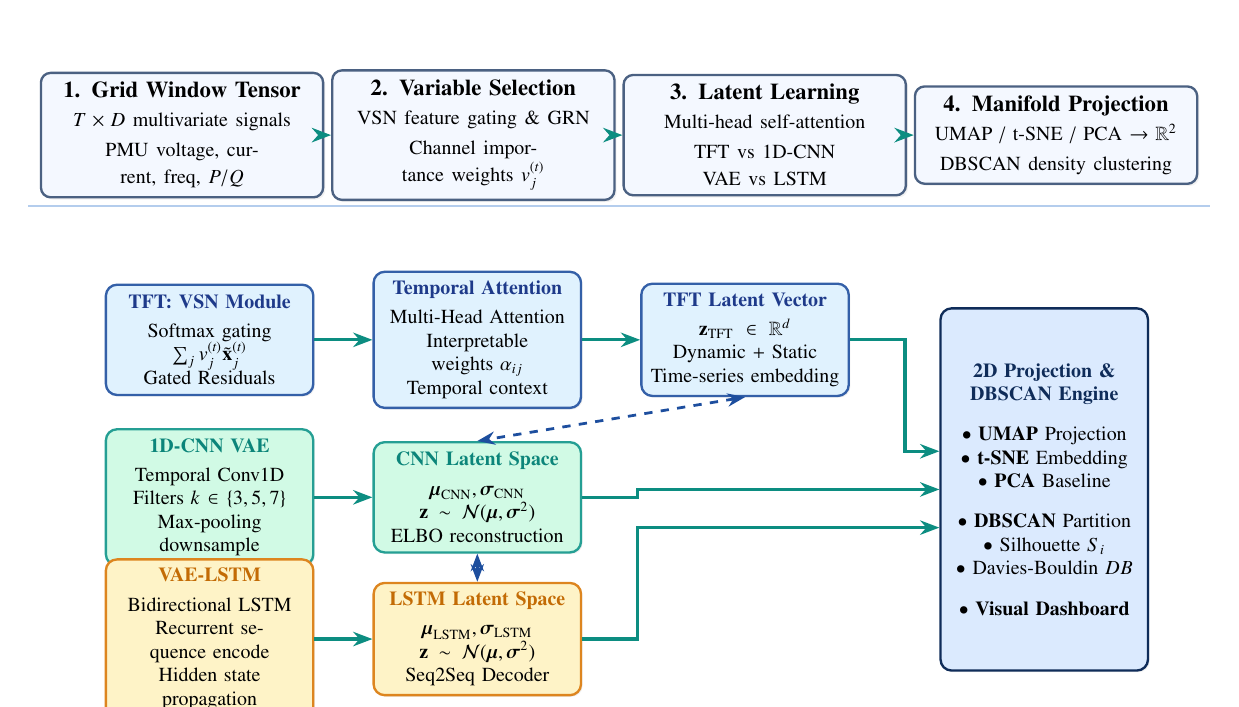
\begin{tikzpicture}[
  x=1cm, y=1cm,
  font=\sffamily,
  dagstep/.style={rectangle, rounded corners=3.5pt, minimum height=1.10cm,
    text width=3.35cm, align=center, draw=lavenderDark!75, fill=lavenderLight!75,
    line width=0.85pt, font=\fontsize{8.2}{9.8}\selectfont\bfseries,
    drop shadow={shadow xshift=0.8pt, shadow yshift=-0.8pt, opacity=0.10}},
  dagarrow/.style={-{Stealth[scale=0.85]}, line width=1.15pt, draw=prismTeal!95!black},
  blkbox/.style={rectangle, rounded corners=4pt, line width=0.85pt,
    minimum height=1.40cm, text width=2.40cm, align=center,
    font=\fontsize{7.2}{8.5}\selectfont, drop shadow={shadow xshift=0.6pt, shadow yshift=-0.6pt, opacity=0.12}},
  transbox/.style={rectangle, rounded corners=3pt, line width=0.80pt,
    draw=prismTeal!80, fill=cStage1!60, minimum height=1.15cm, text width=1.45cm, align=center,
    font=\fontsize{6.5}{7.6}\selectfont},
  skipconn/.style={-{Stealth[scale=0.75]}, line width=0.85pt, draw=prismNavy, dashed}
]

  % Row 1: 4-Stage Architectural Progression
  \node[dagstep] (s1) at (-5.55, 0) {1. Grid Window Tensor\\[2pt]\normalfont\fontsize{7.2}{8.5}\selectfont $T \times D$ multivariate signals\\[1pt]PMU voltage, current, freq, $P/Q$};
  \node[dagstep] (s2) at (-1.85, 0) {2. Variable Selection\\[2pt]\normalfont\fontsize{7.2}{8.5}\selectfont VSN feature gating \& GRN\\[1pt]Channel importance weights $v_j^{(t)}$};
  \node[dagstep] (s3) at (1.85, 0) {3. Latent Learning\\[2pt]\normalfont\fontsize{7.2}{8.5}\selectfont Multi-head self-attention\\[1pt]TFT vs 1D-CNN VAE vs LSTM};
  \node[dagstep] (s4) at (5.55, 0) {4. Manifold Projection\\[2pt]\normalfont\fontsize{7.2}{8.5}\selectfont UMAP / t-SNE / PCA $\to \mathbb{R}^2$\\[1pt]DBSCAN density clustering};

  \draw[dagarrow] (s1) -- (s2);
  \draw[dagarrow] (s2) -- (s3);
  \draw[dagarrow] (s3) -- (s4);

  % Separator
  \draw[draw=lavenderBorder, line width=0.6pt] (-7.5, -0.90) -- (7.5, -0.90);

  % Row 2 & 3: Detailed Architecture Branches
  % Branch 1: TFT (Primary)
  \node[blkbox, draw=prismBlue!90, fill=cStem] (b_tft_vsn) at (-5.20, -2.60) {
    \textbf{\color{prismIndigo}TFT: VSN Module}\\[2pt]
    Softmax gating\\
    $\sum_j v_j^{(t)} \tilde{\mathbf{x}}_j^{(t)}$\\
    Gated Residuals
  };

  \node[blkbox, draw=prismBlue!90, fill=cStem] (b_tft_attn) at (-1.80, -2.60) {
    \textbf{\color{prismIndigo}Temporal Attention}\\[2pt]
    Multi-Head Attention\\
    Interpretable weights $\alpha_{ij}$\\
    Temporal context
  };

  \node[blkbox, draw=prismBlue!90, fill=cStem] (b_tft_latent) at (1.60, -2.60) {
    \textbf{\color{prismIndigo}TFT Latent Vector}\\[2pt]
    $\mathbf{z}_{\text{TFT}} \in \mathbb{R}^d$\\
    Dynamic + Static\\
    Time-series embedding
  };

  \draw[dagarrow] (b_tft_vsn) -- (b_tft_attn);
  \draw[dagarrow] (b_tft_attn) -- (b_tft_latent);

  % Branch 2: 1D-CNN VAE (Baseline 1)
  \node[blkbox, draw=prismTeal!90, fill=cStage1] (b_cnn_vae) at (-5.20, -4.60) {
    \textbf{\color{prismTeal!90!black}1D-CNN VAE}\\[2pt]
    Temporal Conv1D\\
    Filters $k \in \{3, 5, 7\}$\\
    Max-pooling downsample
  };

  \node[blkbox, draw=prismTeal!90, fill=cStage1] (b_cnn_latent) at (-1.80, -4.60) {
    \textbf{\color{prismTeal!90!black}CNN Latent Space}\\[2pt]
    $\boldsymbol{\mu}_{\text{CNN}}, \boldsymbol{\sigma}_{\text{CNN}}$\\
    $\mathbf{z} \sim \mathcal{N}(\boldsymbol{\mu}, \boldsymbol{\sigma}^2)$\\
    ELBO reconstruction
  };

  \draw[dagarrow] (b_cnn_vae) -- (b_cnn_latent);

  % Branch 3: VAE-LSTM (Baseline 2)
  \node[blkbox, draw=prismGold!90, fill=cStage2] (b_lstm_vae) at (-5.20, -6.40) {
    \textbf{\color{prismGold!90!black}VAE-LSTM}\\[2pt]
    Bidirectional LSTM\\
    Recurrent sequence encode\\
    Hidden state propagation
  };

  \node[blkbox, draw=prismGold!90, fill=cStage2] (b_lstm_latent) at (-1.80, -6.40) {
    \textbf{\color{prismGold!90!black}LSTM Latent Space}\\[2pt]
    $\boldsymbol{\mu}_{\text{LSTM}}, \boldsymbol{\sigma}_{\text{LSTM}}$\\
    $\mathbf{z} \sim \mathcal{N}(\boldsymbol{\mu}, \boldsymbol{\sigma}^2)$\\
    Seq2Seq Decoder
  };

  \draw[dagarrow] (b_lstm_vae) -- (b_lstm_latent);

  % Unified Projection & Clustering Engine
  \node[blkbox, draw=lavenderDark, fill=cHead, minimum height=4.60cm, text width=2.40cm] (b_proj) at (5.40, -4.50) {
    \textbf{\color{lavenderDark}2D Projection \&}\\
    \textbf{\color{lavenderDark}DBSCAN Engine}\\[6pt]
    $\bullet$ \textbf{UMAP} Projection\\
    $\bullet$ \textbf{t-SNE} Embedding\\
    $\bullet$ \textbf{PCA} Baseline\\[6pt]
    $\bullet$ \textbf{DBSCAN} Partition\\
    $\bullet$ Silhouette $S_i$\\
    $\bullet$ Davies-Bouldin $DB$\\[6pt]
    $\bullet$ \textbf{Visual Dashboard}
  };

  % Convergence connections to Unified Engine
  \draw[dagarrow] (b_tft_latent.east) -- ++(0.7, 0) |- (b_proj.160);
  \draw[dagarrow] (b_cnn_latent.east) -- ++(0.7, 0) |- (b_proj.west);
  \draw[dagarrow] (b_lstm_latent.east) -- ++(0.7, 0) |- (b_proj.200);

  % Inter-model comparison link
  \draw[{Stealth[scale=0.85]}-{Stealth[scale=0.85]}, line width=1.0pt, dashed, draw=lavenderMedium]
    (b_tft_latent.south) -- (b_cnn_latent.north);
  \draw[{Stealth[scale=0.85]}-{Stealth[scale=0.85]}, line width=1.0pt, dashed, draw=lavenderMedium]
    (b_cnn_latent.south) -- (b_lstm_latent.north);

\end{tikzpicture}
\end{document}
}
    \caption{Structural decomposition of the Temporal Fusion Transformer (TFT) with Variable Selection Networks, comparative VAE pipelines, and the 2D projection clustering engine.}
    \label{fig:dag_scheduling_walkthrough}
\end{figure}

\section{Detailed Component Analysis}

\subsection{Data Storage, Model Artifacts, and Schema Connectors}
Figure~\ref{fig:db_schema} depicts the relational schema architecture connecting raw grid telemetry, latent representations, 2D coordinates, cluster partitions, event annotations, and HITL evaluations.

\begin{figure}[H]
    \centering
    \adjustbox{max width=0.98\linewidth, max height=0.72\textheight, keepaspectratio, center}{\documentclass[tikz,border=10pt]{standalone}
\usepackage{tikz}
\usepackage{fontawesome5}
\usepackage{amsmath,amssymb}
\usetikzlibrary{arrows.meta,positioning,fit,backgrounds,calc,shadows,shapes.geometric}

% Color definitions
\definecolor{lavenderDark}{RGB}{15, 44, 89}
\definecolor{lavenderDeep}{RGB}{10, 28, 58}
\definecolor{lavenderMedium}{RGB}{29, 78, 158}
\definecolor{lavenderLight}{RGB}{240, 246, 255}
\definecolor{lavenderBorder}{RGB}{180, 205, 237}
\definecolor{prismTeal}{RGB}{13, 148, 136}
\definecolor{prismMint}{RGB}{236, 253, 245}
\definecolor{prismGold}{RGB}{217, 119, 6}
\definecolor{prismDark}{RGB}{15, 23, 42}
\definecolor{prismBlue}{RGB}{29, 78, 158}
\definecolor{cInput}{RGB}{241, 245, 249}
\definecolor{cPlanner}{RGB}{219, 234, 254}
\definecolor{cReact}{RGB}{209, 250, 229}
\definecolor{cTool}{RGB}{254, 243, 199}
\definecolor{cSafety}{RGB}{254, 226, 226}
\definecolor{cDeliverable}{RGB}{204, 251, 241}

\begin{document}
% Relational Entity & Storage Schema Connectors for Power Grid Event Diagnosis
\begin{tikzpicture}[
  x=1cm, y=1cm,
  font=\sffamily,
  tblcard/.style={
    rectangle, rounded corners=4pt, draw=lavenderDark!75, line width=0.85pt, fill=white,
    inner sep=5pt, text width=4.50cm, align=left,
    drop shadow={shadow xshift=1pt, shadow yshift=-1pt, opacity=0.12}
  },
  fkarrow/.style={
    -{Stealth[scale=0.85]}, line width=1.0pt, draw=lavenderDark!90
  },
  fklabel/.style={
    font=\fontsize{6.2}{7.2}\selectfont\bfseries, fill=white, inner sep=1.5pt, text=lavenderDark
  }
]

  % ================= COLUMN 1: SIGNALS & LATENT REPS (x = -5.4) =================
  
  % Table 1: grid_signal_store
  \node[tblcard] (signals) at (-5.4, 2.5) {%
    \centerline{\color{lavenderDark}\faBolt\ \textbf{\fontsize{8.0}{9.5}\selectfont grid\_signal\_store}}\\[3pt]
    \rule{\linewidth}{0.4pt}\\[3pt]
    {\fontsize{6.8}{8.0}\selectfont
    \textbf{\color{lavenderDark}[PK]} \texttt{signal\_id}: \textit{UUID} (Indexed)\\
    \textbf{\color{prismTeal}[FLD]} \texttt{bus\_id}: \textit{integer} (Substation Bus)\\
    \textbf{\color{prismTeal}[FLD]} \texttt{timestamp}: \textit{datetime} (GPS Synced)\\
    \textbf{\color{prismDark!80}[FLD]} \texttt{voltage\_mag}, \texttt{current\_mag}: \textit{float}\\
    \textbf{\color{prismDark!80}[FLD]} \texttt{frequency}, \texttt{phase\_angle}: \textit{float}\\
    \textbf{\color{prismDark!80}[FLD]} \texttt{active\_P}, \texttt{reactive\_Q}: \textit{float}}
  };

  % Table 2: latent_representation_store
  \node[tblcard, below=0.70cm of signals] (latent) {%
    \centerline{\color{lavenderDark}\faBrain\ \textbf{\fontsize{8.0}{9.5}\selectfont latent\_representation\_store}}\\[3pt]
    \rule{\linewidth}{0.4pt}\\[3pt]
    {\fontsize{6.8}{8.0}\selectfont
    \textbf{\color{lavenderDark}[PK]} \texttt{latent\_id}: \textit{UUID}\\
    \textbf{\color{prismBlue}[FK]} \texttt{signal\_id} $\rightarrow$ \texttt{grid\_signal.signal\_id}\\
    \textbf{\color{prismTeal}[FLD]} \texttt{model\_type}: \textit{TFT / CNN-VAE / LSTM}\\
    \textbf{\color{prismDark!80}[FLD]} \texttt{embedding\_vector}: \textit{float[$d$] ($d=128$)}\\
    \textbf{\color{prismDark!80}[FLD]} \texttt{reconstruction\_loss}: \textit{float}\\
    \textbf{\color{prismDark!80}[FLD]} \texttt{vsn\_weights}: \textit{json (Variable weights)}}
  };

  % ================= COLUMN 2: 2D PROJECTIONS & CLUSTERS (x = 0.0) =================

  % Table 3: projection_coordinate_store
  \node[tblcard] (proj) at (0.0, 2.5) {%
    \centerline{\color{lavenderDark}\faCompress\ \textbf{\fontsize{8.0}{9.5}\selectfont projection\_coordinate\_store}}\\[3pt]
    \rule{\linewidth}{0.4pt}\\[3pt]
    {\fontsize{6.8}{8.0}\selectfont
    \textbf{\color{lavenderDark}[PK]} \texttt{proj\_id}: \textit{UUID}\\
    \textbf{\color{prismBlue}[FK]} \texttt{latent\_id} $\rightarrow$ \texttt{latent\_rep.latent\_id}\\
    \textbf{\color{prismTeal}[FLD]} \texttt{method}: \textit{UMAP / t-SNE / PCA}\\
    \textbf{\color{prismDark!80}[FLD]} \texttt{coord\_x}: \textit{float (2D map coordinate)}\\
    \textbf{\color{prismDark!80}[FLD]} \texttt{coord\_y}: \textit{float (2D map coordinate)}\\
    \textbf{\color{prismDark!80}[FLD]} \texttt{hyperparams}: \textit{json ($n\_neighbors, min\_dist$)}}
  };

  % Table 4: cluster_partition_store
  \node[tblcard, below=0.70cm of proj] (cluster) {%
    \centerline{\color{lavenderDark}\faProjectDiagram\ \textbf{\fontsize{8.0}{9.5}\selectfont cluster\_partition\_store}}\\[3pt]
    \rule{\linewidth}{0.4pt}\\[3pt]
    {\fontsize{6.8}{8.0}\selectfont
    \textbf{\color{lavenderDark}[PK]} \texttt{cluster\_id}: \textit{UUID}\\
    \textbf{\color{prismBlue}[FK]} \texttt{proj\_id} $\rightarrow$ \texttt{projection.proj\_id}\\
    \textbf{\color{prismTeal}[FLD]} \texttt{algorithm}: \textit{DBSCAN}\\
    \textbf{\color{prismDark!80}[FLD]} \texttt{eps\_radius}, \texttt{min\_pts}: \textit{float, int}\\
    \textbf{\color{prismDark!80}[FLD]} \texttt{cluster\_label}: \textit{integer (-1: Noise)}\\
    \textbf{\color{prismDark!80}[FLD]} \texttt{silhouette\_score}: \textit{float ($S_i$)}}
  };

  % ================= COLUMN 3: EVENT ANNOTATIONS & HITL (x = 5.4) =================

  % Table 5: event_annotation_store
  \node[tblcard] (events) at (5.4, 2.5) {%
    \centerline{\color{lavenderDark}\faExclamationCircle\ \textbf{\fontsize{8.0}{9.5}\selectfont event\_annotation\_store}}\\[3pt]
    \rule{\linewidth}{0.4pt}\\[3pt]
    {\fontsize{6.8}{8.0}\selectfont
    \textbf{\color{lavenderDark}[PK]} \texttt{event\_id}: \textit{UUID}\\
    \textbf{\color{prismBlue}[FK]} \texttt{cluster\_id} $\rightarrow$ \texttt{cluster.cluster\_id}\\
    \textbf{\color{prismTeal}[FLD]} \texttt{event\_category}: \textit{Fault / Trip / Oscil}\\
    \textbf{\color{prismDark!80}[FLD]} \texttt{severity\_level}: \textit{1 to 5}\\
    \textbf{\color{prismDark!80}[FLD]} \texttt{affected\_substations}: \textit{list[string]}\\
    \textbf{\color{prismDark!80}[FLD]} \texttt{timestamp\_onset}: \textit{datetime}}
  };

  % Table 6: hitl_evaluation_store
  \node[tblcard, below=0.70cm of events] (hitl) {%
    \centerline{\color{lavenderDark}\faUserCheck\ \textbf{\fontsize{8.0}{9.5}\selectfont hitl\_evaluation\_store}}\\[3pt]
    \rule{\linewidth}{0.4pt}\\[3pt]
    {\fontsize{6.8}{8.0}\selectfont
    \textbf{\color{lavenderDark}[PK]} \texttt{eval\_id}: \textit{UUID}\\
    \textbf{\color{prismBlue}[FK]} \texttt{event\_id} $\rightarrow$ \texttt{event\_annotation.event\_id}\\
    \textbf{\color{prismTeal}[FLD]} \texttt{expert\_operator\_id}: \textit{string}\\
    \textbf{\color{prismDark!80}[FLD]} \texttt{validation\_status}: \textit{Approved / Flagged}\\
    \textbf{\color{prismDark!80}[FLD]} \texttt{davies\_bouldin\_idx}: \textit{float ($DB$)}\\
    \textbf{\color{prismDark!80}[FLD]} \texttt{feedback\_notes}: \textit{text}}
  };

  % Foreign Key Connections
  \draw[fkarrow] (signals.south) -- (latent.north)
    node[midway, right=1pt, fklabel]{1:N Signals};

  \draw[fkarrow] (latent.east) -- (proj.west)
    node[midway, above=1pt, fklabel]{1:N Proj};

  \draw[fkarrow] (proj.south) -- (cluster.north)
    node[midway, right=1pt, fklabel]{1:N Clusters};

  \draw[fkarrow] (cluster.east) -- (events.west)
    node[midway, above=1pt, fklabel]{1:N Events};

  \draw[fkarrow] (events.south) -- (hitl.north)
    node[midway, right=1pt, fklabel]{1:N HITL};

\end{tikzpicture}
\end{document}
}
    \caption{Relational entity and data storage schema connectors showing grid signals, latent embeddings, projection coordinates, cluster partitions, event annotations, and HITL feedback.}
    \label{fig:db_schema}
\end{figure}

\subsection{Level-1 Data Flow Architecture}
Figure~\ref{fig:data_flow_diagram} illustrates the Level-1 Data Flow Diagram (DFD), showing external entities, primary processing transformations, datastores, and human feedback loops.

\begin{figure}[H]
    \centering
    \adjustbox{max width=0.98\linewidth, max height=0.72\textheight, keepaspectratio, center}{\documentclass[tikz,border=12pt]{standalone}
\usepackage{tikz}
\usepackage{amsmath,amssymb}
\usepackage{fontawesome5}
\usetikzlibrary{arrows.meta,positioning,fit,backgrounds,calc,shadows,shapes.geometric}

% Color definitions
\definecolor{lavenderDark}{RGB}{15, 44, 89}
\definecolor{lavenderDeep}{RGB}{10, 28, 58}
\definecolor{lavenderMedium}{RGB}{29, 78, 158}
\definecolor{lavenderLight}{RGB}{240, 246, 255}
\definecolor{lavenderBorder}{RGB}{180, 205, 237}
\definecolor{prismNavy}{RGB}{15, 44, 89}
\definecolor{prismBlue}{RGB}{29, 78, 158}
\definecolor{prismTeal}{RGB}{13, 148, 136}
\definecolor{prismGold}{RGB}{217, 119, 6}
\definecolor{prismDark}{RGB}{15, 23, 42}
\definecolor{cInput}{RGB}{241, 245, 249}
\definecolor{cStem}{RGB}{224, 242, 254}
\definecolor{cStage1}{RGB}{209, 250, 229}
\definecolor{cStage2}{RGB}{254, 243, 199}
\definecolor{cStage4}{RGB}{207, 250, 254}
\definecolor{cHead}{RGB}{219, 234, 254}

\begin{document}
% Level-1 Data Flow Diagram (DFD) for Power Grid Visual Analytics
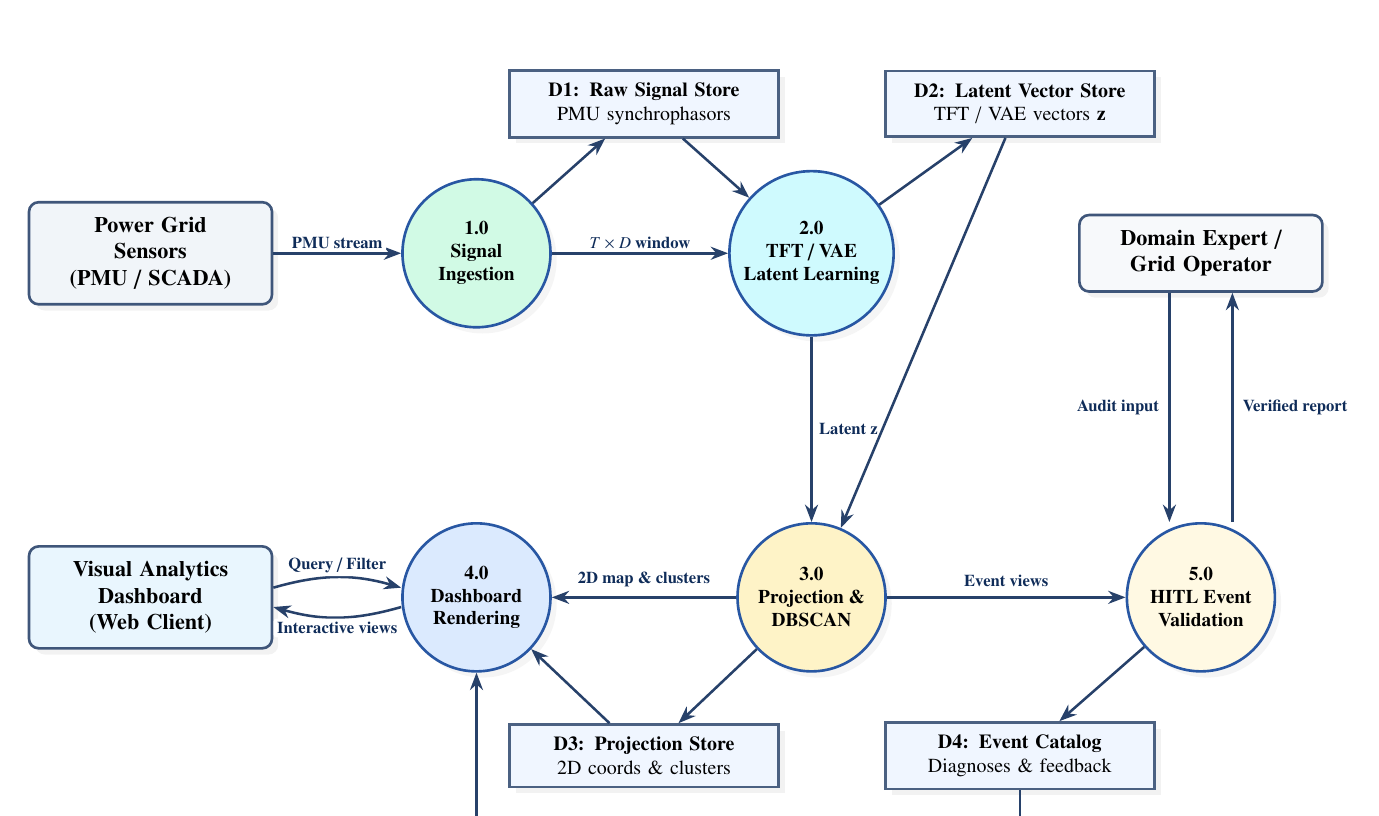
\begin{tikzpicture}[
  x=1.15cm, y=1.15cm,
  font=\sffamily,
  entity/.style={
    rectangle, draw=lavenderDark!80, line width=0.95pt, rounded corners=3.5pt,
    align=center, inner sep=5.5pt, font=\fontsize{8.0}{9.5}\selectfont\bfseries,
    text width=2.70cm, fill=cInput, drop shadow={opacity=0.10}
  },
  store/.style={
    rectangle, draw=lavenderDark!75, line width=0.95pt,
    align=center, inner sep=4.5pt, font=\fontsize{7.2}{8.6}\selectfont,
    text width=3.10cm, fill=lavenderLight, drop shadow={opacity=0.10}
  },
  proc/.style={
    circle, draw=lavenderMedium!95, line width=0.95pt,
    align=center, inner sep=2pt, minimum size=1.88cm,
    font=\fontsize{7.0}{8.3}\selectfont\bfseries, fill=cStage1, drop shadow={opacity=0.08}
  },
  procblue/.style={proc, fill=cStage4},
  procgold/.style={proc, fill=cStage2},
  prochead/.style={proc, fill=cHead},
  dfdarr/.style={
    -{Stealth[scale=0.88]}, line width=0.92pt, draw=lavenderDark!90
  },
  flowlbl/.style={
    font=\fontsize{6.0}{7.2}\selectfont\bfseries, fill=white, inner sep=1.3pt, text=lavenderDark, rounded corners=1pt
  }
]

  % External Entities
  \node[entity] (sensors) at (-5.8, 3.2) {Power Grid\\Sensors\\(PMU / SCADA)};
  \node[entity, fill=cStem!70] (ui) at (-5.8, -0.6) {Visual Analytics\\Dashboard\\(Web Client)};
  \node[entity, fill=cInput!60] (expert) at (5.8, 3.2) {Domain Expert /\\Grid Operator};

  % Processes
  \node[proc] (p1) at (-2.2, 3.2) {1.0\\Signal\\Ingestion};
  \node[procblue] (p2) at (1.5, 3.2) {2.0\\TFT / VAE\\Latent Learning};
  \node[procgold] (p3) at (1.5, -0.6) {3.0\\Projection \&\\DBSCAN};
  \node[prochead] (p4) at (-2.2, -0.6) {4.0\\Dashboard\\Rendering};
  \node[proc, fill=cStage2!50] (p5) at (5.8, -0.6) {5.0\\HITL Event\\Validation};

  % Data Stores (D1-D4 in standard quadrant order)
  \node[store] (d1) at (-0.35, 4.85) {\textbf{D1: Raw Signal Store}\\PMU synchrophasors};
  \node[store] (d2) at (3.8, 4.85) {\textbf{D2: Latent Vector Store}\\TFT / VAE vectors $\mathbf{z}$};
  \node[store] (d3) at (-0.35, -2.35) {\textbf{D3: Projection Store}\\2D coords \& clusters};
  \node[store] (d4) at (3.8, -2.35) {\textbf{D4: Event Catalog}\\Diagnoses \& feedback};

  % Data Flows - Top Row
  \draw[dfdarr] (sensors) -- node[above, flowlbl]{PMU stream} (p1);
  \draw[dfdarr] (p1) -- node[above, flowlbl]{$T \times D$ window} (p2);
  \draw[dfdarr] (p1) -- (d1);
  \draw[dfdarr] (d1) -- (p2);

  % Latent Flows
  \draw[dfdarr] (p2) -- node[right=1pt, flowlbl]{Latent $\mathbf{z}$} (p3);
  \draw[dfdarr] (p2) -- (d2);
  \draw[dfdarr] (d2) -- (p3);

  % Process 3.0 outputs (branching left to Dashboard, right to HITL)
  \draw[dfdarr] (p3) -- node[above=2pt, midway, flowlbl]{2D map \& clusters} (p4);
  \draw[dfdarr] (p3) -- (d3);
  \draw[dfdarr] (d3) -- (p4);
  \draw[dfdarr] (p3) -- node[above=2pt, midway, flowlbl]{Event views} (p5);

  % UI <-> Dashboard Rendering (Curved bidirectional paths with separated anchors)
  \draw[dfdarr] ([yshift=3.5pt]ui.east) to[bend left=16] node[above, flowlbl]{Query / Filter} ([yshift=3.5pt]p4.west);
  \draw[dfdarr] ([yshift=-3.5pt]p4.west) to[bend left=16] node[below, flowlbl]{Interactive views} ([yshift=-3.5pt]ui.east);

  % Domain Expert <-> HITL Validation (Separated parallel bidirectional flows)
  \draw[dfdarr] ([xshift=-0.40cm]expert.south) -- node[left=2pt, flowlbl]{Audit input} ([xshift=-0.40cm]p5.north);
  \draw[dfdarr] ([xshift=0.40cm]p5.north) -- node[right=2pt, flowlbl]{Verified report} ([xshift=0.40cm]expert.south);

  % HITL Feedback to Event Catalog & Dashboard
  \draw[dfdarr] (p5) -- (d4);
  \draw[dfdarr] (d4.south) -- ++(0, -0.42) -| (p4.south);

\end{tikzpicture}
\end{document}
}
    \caption{Level-1 Data Flow Diagram (DFD) depicting external entities, representation transformations, datastores, and the visual feedback loop.}
    \label{fig:data_flow_diagram}
\end{figure}


%==============================================================================
% CHAPTER 6: DESIGN AND METHODOLOGY
%==============================================================================
\chapter{Design and Methodology}

This chapter details the mathematical formulations, system methodology, comparative training configurations, projection engines, and visual dashboard interfaces realizing the explainable visual analytics framework.

\section{Temporal Fusion Transformer (TFT) Methodology}
The Temporal Fusion Transformer is configured specifically for multivariate power grid time series. Given a framed sequence $\mathbf{X} \in \mathbb{R}^{T \times D}$, each continuous input feature $x_{t, j}$ is projected into a $d_{\text{model}}$-dimensional vector space using a linear transformation:
\begin{equation}
    \tilde{\mathbf{x}}_{t, j} = \mathbf{W}_j x_{t, j} + \mathbf{b}_j, \quad \tilde{\mathbf{x}}_{t, j} \in \mathbb{R}^{d_{\text{model}}}
\end{equation}

\subsection{Gated Residual Network (GRN)}
The core building block within TFT is the Gated Residual Network (GRN), which provides adaptive non-linear processing and skip connections:
\begin{equation}
    \text{GRN}_\omega(\mathbf{a}, \mathbf{c}) = \text{LayerNorm}\left( \mathbf{a} + \text{GLU}_\omega\left( \mathbf{W}_{1, \omega} \mathbf{\eta}_1 + \mathbf{b}_{1, \omega} \right) \right)
\end{equation}
where $\mathbf{\eta}_1 = \text{ELU}(\mathbf{W}_{2, \omega} \mathbf{a} + \mathbf{W}_{3, \omega} \mathbf{c} + \mathbf{b}_{2, \omega})$, and $\text{GLU}_\omega(\boldsymbol{\gamma}) = \boldsymbol{\gamma}_1 \odot \sigma(\boldsymbol{\gamma}_2)$ represents the Gated Linear Unit providing component-level gating.

\subsection{Interpretable Multi-Head Self-Attention}
TFT modifies standard multi-head self-attention by sharing value weights across heads, ensuring that attention weights $\alpha_{ij}$ directly reflect the temporal importance of past time steps. The attention head output is:
\begin{equation}
    \mathbf{h}_i = \sum_{j=1}^T \tilde{\alpha}_{ij} \mathbf{V} \tilde{\mathbf{x}}_j
\end{equation}
where $\tilde{\alpha}_{ij} = \frac{1}{H} \sum_{m=1}^H \alpha_{ij}^{(m)}$ represents the head-averaged attention weight. The pooled output forms the latent vector $\mathbf{z}_{\text{TFT}} \in \mathbb{R}^d$.

\section{Variational Autoencoder (VAE) Baseline Architectures}

\subsection{1D-CNN VAE Baseline}
The 1D-CNN VAE applies temporal convolutions across the channel dimension. The encoder comprises three sequential 1D convolutional layers with batch normalization and LeakyReLU activations:
\begin{align}
    \mathbf{H}^{(1)} &= \text{LeakyReLU}\big(\text{Conv1D}_{k=7}(\tilde{\mathbf{X}})\big) \\
    \mathbf{H}^{(2)} &= \text{LeakyReLU}\big(\text{Conv1D}_{k=5}(\mathbf{H}^{(1)})\big) \\
    \mathbf{H}^{(3)} &= \text{LeakyReLU}\big(\text{Conv1D}_{k=3}(\mathbf{H}^{(2)})\big)
\end{align}
The flattened tensor parameterizes the Gaussian posterior:
\begin{equation}
    \boldsymbol{\mu} = \mathbf{W}_\mu \text{vec}(\mathbf{H}^{(3)}) + \mathbf{b}_\mu, \quad \log \boldsymbol{\sigma}^2 = \mathbf{W}_\sigma \text{vec}(\mathbf{H}^{(3)}) + \mathbf{b}_\sigma
\end{equation}
The decoder mirrors this architecture using transposed 1D convolutions to reconstruct $\hat{\mathbf{X}}$.

\subsection{VAE-LSTM Baseline}
The VAE-LSTM utilizes a 2-layer Bidirectional LSTM. For sequence $[\tilde{\mathbf{x}}_1, \dots, \tilde{\mathbf{x}}_T]$, forward states $\vec{\mathbf{h}}_t$ and backward states $\overleftarrow{\mathbf{h}}_t$ are generated:
\begin{equation}
    \mathbf{h}_t = [\vec{\mathbf{h}}_t \,;\, \overleftarrow{\mathbf{h}}_t]
\end{equation}
The terminal state $\mathbf{h}_T$ parameterizes the latent distribution: $\boldsymbol{\mu} = \mathbf{W}_\mu \mathbf{h}_T + \mathbf{b}_\mu$, $\log \boldsymbol{\sigma}^2 = \mathbf{W}_\sigma \mathbf{h}_T + \mathbf{b}_\sigma$. The decoder consists of a unidirectional LSTM initialized with sampled vector $\mathbf{z}$, autoregressively reconstructing the original time-series sequence.

\section{Model Training and Hyperparameter Configuration}
Table~\ref{tab:model_hyperparameters} details the comparative training hyperparameters employed across the three architectures.

\section{Dataset Description and Configuration Verification}
The report describes a GESL power-grid time-series dataset and uses the configuration $T=128$, $D=24$, with a stated total of 15,000 windows and stride $S=10$. The supplied project folder was inspected recursively, including source code, configuration, dataset-loading, training, evaluation, checkpoint, and output files. That inspection found a lung-detection image-classification application under 	exttt{codebase/lung-detection}, not a GESL power-grid implementation. Its loader uses 	exttt{ImageFolder}, the classes 	exttt{Normal}, 	exttt{COVID}, and 	exttt{Viral Pneumonia}, 224$	imes$224 RGB images, ImageNet normalization, and a 70/15/15 stratified image split. These files are unrelated to the GESL claims and cannot verify them.

The GESL provider, original source or publication, covered time period, selected subset or event categories, 24 feature names and meanings, normalization statistics, missing-value policy, temporal ordering, window derivation, and power-grid train--validation--test split therefore remain 	extbf{Requires verification}. The report values $T=128$, $D=24$, 15,000 windows, and $S=10$ are retained only as stated configuration claims. No GESL implementation evidence was found from which to derive the window count, identify the 24 channels, or test for leakage from overlapping windows.

\begin{tcolorbox}[colback=lavenderLight,colframe=lavenderBorder,title=Verification note]
Dataset origin, feature list, time coverage, window-count derivation, preprocessing, split, and model-output evidence remain \textbf{pending source-code/dataset verification}. No new dataset details have been invented in this revision.
\end{tcolorbox}

\begin{table}[H]
\centering
\scriptsize
\caption{Dataset configuration summary based on the supplied evidence. ``Requires verification'' denotes a field for which no GESL source or power-grid implementation artifact was available.}
\label{tab:dataset_verification_summary}
\begin{tabularx}{\textwidth}{>{\raggedright\arraybackslash}p{2.0cm} >{\raggedright\arraybackslash}p{2.1cm} >{\raggedright\arraybackslash}p{1.3cm} >{\raggedright\arraybackslash}p{1.4cm} X >{\raggedright\arraybackslash}p{2.6cm}}
\toprule
\textbf{Source / role} & \textbf{Samples or windows} & \textbf{Features} & \textbf{Length} & \textbf{Preprocessing} & \textbf{Split / status} \\
\midrule
GESL power-grid data claimed by the report & 15,000 windows (claimed; not observed) & $D=24$ (claimed; names unavailable) & $T=128$, $S=10$ (claimed) & Missing-value handling, cleaning, normalization, feature selection, temporal ordering, and event subset: \textbf{Requires verification} & Provider, official reference, split method/counts, and leakage check: \textbf{Requires verification} \\
\addlinespace
Supplied implementation (lung-detection) & Image samples; GESL windows not present & 224$\times$224 RGB image input; not $D=24$ & Not applicable & Image validation, resize, augmentation during training, ImageNet normalization & 70\% / 15\% / 15\% stratified image split; unrelated to GESL \\
\bottomrule
\end{tabularx}
\end{table}

\begin{table}[H]
\centering
\small
\caption{Model architecture and training hyperparameters.}
\label{tab:model_hyperparameters}
\begin{tabularx}{\textwidth}{>{\raggedright\arraybackslash}p{4.0cm} >{\raggedright\arraybackslash}X >{\raggedright\arraybackslash}X >{\raggedright\arraybackslash}X}
\toprule
\textbf{Hyperparameter} & \textbf{TFT} & \textbf{1D-CNN VAE} & \textbf{VAE-LSTM} \\
\midrule
Input Dimension ($T \times D$) & $128 \times 24$ & $128 \times 24$ & $128 \times 24$ \\
Latent Dimension ($d$) & 128 & 128 & 128 \\
Hidden Units / Channels & $d_{\text{model}}=64$ & Channels: 32, 64, 128 & Hidden size: 128 (2 layers) \\
Attention Heads & 4 & N/A & N/A \\
Optimizer & AdamW & Adam & Adam \\
Learning Rate & $10^{-3}$ (Cosine decay) & $10^{-3}$ & $5 \times 10^{-4}$ \\
Weight Decay & $10^{-4}$ & $10^{-5}$ & $10^{-5}$ \\
Batch Size & 64 & 64 & 64 \\
Dropout Rate & 0.15 & 0.20 & 0.20 \\
Loss Function & Quantile + MSE & ELBO ($\beta$-VAE, $\beta=0.5$) & ELBO ($\beta$-VAE, $\beta=0.5$) \\
Training Epochs & 50 & 50 & 50 \\
Early Stopping Patience & 8 epochs & 8 epochs & 8 epochs \\
\bottomrule
\end{tabularx}
\end{table}

\section{Model Responsibilities and Staged Inference Flow}
Figure~\ref{fig:ml_inference_flow} delineates the six specialized operational stages executed during feature extraction and diagnostic inference.

\begin{figure}[H]
    \centering
    \adjustbox{max width=0.98\linewidth, max height=0.72\textheight, keepaspectratio, center}{\documentclass[tikz,border=10pt]{standalone}
\usepackage{tikz}
\usepackage{fontawesome5}
\usepackage{amsmath,amssymb}
\usetikzlibrary{arrows.meta,positioning,fit,backgrounds,calc,shadows,shapes.geometric}

% Color definitions
\definecolor{lavenderDark}{RGB}{15, 44, 89}
\definecolor{lavenderDeep}{RGB}{10, 28, 58}
\definecolor{lavenderMedium}{RGB}{29, 78, 158}
\definecolor{lavenderLight}{RGB}{240, 246, 255}
\definecolor{lavenderBorder}{RGB}{180, 205, 237}
\definecolor{prismNavy}{RGB}{15, 44, 89}
\definecolor{prismBlue}{RGB}{29, 78, 158}
\definecolor{prismTeal}{RGB}{13, 148, 136}
\definecolor{prismGold}{RGB}{217, 119, 6}
\definecolor{prismDark}{RGB}{15, 23, 42}
\definecolor{cInput}{RGB}{241, 245, 249}
\definecolor{cStem}{RGB}{224, 242, 254}
\definecolor{cStage1}{RGB}{209, 250, 229}
\definecolor{cStage2}{RGB}{254, 243, 199}
\definecolor{cStage4}{RGB}{207, 250, 254}
\definecolor{cHead}{RGB}{219, 234, 254}

\begin{document}
% Model Responsibilities & Staged Execution Flow for Power Grid Event Diagnosis
\begin{tikzpicture}[
    x=1cm, y=1cm, font=\sffamily,
    modelrow/.style={rectangle, rounded corners=3.5pt, draw=lavenderDark!45,
      line width=0.65pt, inner sep=4.5pt},
    arrow/.style={-{Stealth[scale=0.8]}, line width=0.9pt, draw=lavenderDark!85}
]

  % Stage 1: Grid Telemetry Ingestion (y = 0.0)
  \node[modelrow, fill=cInput!70, text width=2.40cm, align=center, minimum height=1.15cm] (m1l) at (-5.85, 0.0)
    {{\fontsize{8.5}{10.2}\selectfont\color{lavenderDark}\faBolt\ \textbf{1. Ingestion}}\\[2pt]
     {\fontsize{7.5}{9.0}\selectfont\texttt{pmu\_streamer}}};
  \node[modelrow, fill=lavenderLight!85, text width=7.40cm, align=left, minimum height=1.15cm] (m1p) at (-0.55, 0.0)
    {\fontsize{7.6}{9.0}\selectfont \textbf{Stream Validation} $\rightarrow$ Check sync timestamps \& sampling rate ($30\text{--}60$\,Hz)\\[2pt]Verify multi-bus voltage, current, and frequency telemetry completeness};
  \node[modelrow, fill=lavenderLight!85, text width=4.10cm, align=left, minimum height=1.15cm] (m1r) at (5.60, 0.0)
    {\fontsize{7.6}{9.0}\selectfont \textbf{Sanitized Stream}\\[2pt]{\fontsize{6.8}{8.0}\selectfont Filters telemetry desync}};

  % Stage 2: Temporal Preprocessing (y = -1.55)
  \node[modelrow, fill=cStage1!65, text width=2.40cm, align=center, minimum height=1.15cm] (m2l) at (-5.85, -1.55)
    {{\fontsize{8.5}{10.2}\selectfont\color{lavenderDark}\faSlidersH\ \textbf{2. Transform}}\\[2pt]
     {\fontsize{7.5}{9.0}\selectfont\texttt{window\_normalizer}}};
  \node[modelrow, fill=lavenderLight!85, text width=7.40cm, align=left, minimum height=1.15cm] (m2p) at (-0.55, -1.55)
    {\fontsize{7.6}{9.0}\selectfont \textbf{Z-Score Normalization} $\rightarrow$ Scale channels: $\mathbf{x}_{\text{norm}} = (\mathbf{x} - \boldsymbol{\mu}) / \boldsymbol{\sigma}$\\[2pt]Sliding window framing to temporal tensor dimensions $(T \times D)$};
  \node[modelrow, fill=lavenderLight!85, text width=4.10cm, align=left, minimum height=1.15cm] (m2r) at (5.60, -1.55)
    {\fontsize{7.6}{9.0}\selectfont \textbf{Framed Grid Tensor}\\[2pt]{\fontsize{6.8}{8.0}\selectfont Tensor $(B, T=128, D)$}};

  % Stage 3: Variable Selection (y = -3.10)
  \node[modelrow, fill=cStage4!65, text width=2.40cm, align=center, minimum height=1.15cm] (m3l) at (-5.85, -3.10)
    {{\fontsize{8.5}{10.2}\selectfont\color{lavenderDark}\faFilter\ \textbf{3. Var Selection}}\\[2pt]
     {\fontsize{7.5}{9.0}\selectfont\texttt{tft\_vsn.py}}};
  \node[modelrow, fill=lavenderLight!85, text width=7.40cm, align=left, minimum height=1.15cm] (m3p) at (-0.55, -3.10)
    {\fontsize{7.6}{9.0}\selectfont \textbf{Feature Gating} $\rightarrow$ Variable Selection Network assigns weights $v_j^{(t)}$\\[2pt]Isolates dominant grid signals (e.g. line current jump vs frequency swing)};
  \node[modelrow, fill=lavenderLight!85, text width=4.10cm, align=left, minimum height=1.15cm] (m3r) at (5.60, -3.10)
    {\fontsize{7.6}{9.0}\selectfont \textbf{Weighted Signals}\\[2pt]{\fontsize{6.8}{8.0}\selectfont Salient channel features}};

  % Stage 4: Latent Learning (y = -4.65)
  \node[modelrow, fill=cStem!75, text width=2.40cm, align=center, minimum height=1.15cm] (m4l) at (-5.85, -4.65)
    {{\fontsize{8.5}{10.2}\selectfont\color{lavenderDark}\faBrain\ \textbf{4. Latent Learn}}\\[2pt]
     {\fontsize{7.5}{9.0}\selectfont\texttt{tft\_vae\_engine}}};
  \node[modelrow, fill=lavenderLight!85, text width=7.40cm, align=left, minimum height=1.15cm] (m4p) at (-0.55, -4.65)
    {\fontsize{7.6}{9.0}\selectfont \textbf{Temporal Attention / VAE Encoding} $\rightarrow$ Multi-Head Self-Attention\\[2pt]Extracts bottleneck latent representations $\mathbf{z} \in \mathbb{R}^d$ ($d=128$)};
  \node[modelrow, fill=lavenderLight!85, text width=4.10cm, align=left, minimum height=1.15cm] (m4r) at (5.60, -4.65)
    {\fontsize{7.6}{9.0}\selectfont \textbf{Latent Vectors $\mathbf{z}$}\\[2pt]{\fontsize{6.8}{8.0}\selectfont TFT vs 1D-CNN vs LSTM}};

  % Stage 5: Manifold Projection (y = -6.20)
  \node[modelrow, fill=cStage2!70, text width=2.40cm, align=center, minimum height=1.15cm] (m5l) at (-5.85, -6.20)
    {{\fontsize{8.5}{10.2}\selectfont\color{lavenderDark}\faCompress\ \textbf{5. Projection}}\\[2pt]
     {\fontsize{7.5}{9.0}\selectfont\texttt{projection\_engine}}};
  \node[modelrow, fill=lavenderLight!85, text width=7.40cm, align=left, minimum height=1.15cm] (m5p) at (-0.55, -6.20)
    {\fontsize{7.6}{9.0}\selectfont \textbf{2D Dimensionality Reduction} $\rightarrow$ Non-linear manifold embedding\\[2pt]Applies UMAP / t-SNE / PCA to map $\mathbf{z} \in \mathbb{R}^d \to \mathbf{p} \in \mathbb{R}^2$};
  \node[modelrow, fill=lavenderLight!85, text width=4.10cm, align=left, minimum height=1.15cm] (m5r) at (5.60, -6.20)
    {\fontsize{7.6}{9.0}\selectfont \textbf{2D Coordinates}\\[2pt]{\fontsize{6.8}{8.0}\selectfont Preserves event topology}};

  % Stage 6: Dashboard & DBSCAN (y = -7.75)
  \node[modelrow, fill=cHead!75, text width=2.40cm, align=center, minimum height=1.15cm] (m6l) at (-5.85, -7.75)
    {{\fontsize{8.5}{10.2}\selectfont\color{lavenderDark}\faChartArea\ \textbf{6. Dashboard}}\\[2pt]
     {\fontsize{7.5}{9.0}\selectfont\texttt{visual\_analytics}}};
  \node[modelrow, fill=lavenderLight!85, text width=7.40cm, align=left, minimum height=1.15cm] (m6p) at (-0.55, -7.75)
    {\fontsize{7.6}{9.0}\selectfont \textbf{Visual Diagnostics \& HITL} $\rightarrow$ DBSCAN density partition ($\epsilon, \text{MinPts}$)\\[2pt]Renders 2D Latent Map, Multi-Label Tree, and Latent Comparison Chart};
  \node[modelrow, fill=lavenderLight!85, text width=4.10cm, align=left, minimum height=1.15cm] (m6r) at (5.60, -7.75)
    {\fontsize{7.6}{9.0}\selectfont \textbf{Diagnosis \& Feedback}\\[2pt]{\fontsize{6.8}{8.0}\selectfont Expert root-cause audit}};

  % Vertical Connections
  \draw[arrow] (m1l) -- (m2l);
  \draw[arrow] (m2l) -- (m3l);
  \draw[arrow] (m3l) -- (m4l);
  \draw[arrow] (m4l) -- (m5l);
  \draw[arrow] (m5l) -- (m6l);

  \draw[arrow] (m1p) -- (m2p);
  \draw[arrow] (m2p) -- (m3p);
  \draw[arrow] (m3p) -- (m4p);
  \draw[arrow] (m4p) -- (m5p);
  \draw[arrow] (m5p) -- (m6p);

  \draw[arrow] (m1r) -- (m2r);
  \draw[arrow] (m2r) -- (m3r);
  \draw[arrow] (m3r) -- (m4r);
  \draw[arrow] (m4r) -- (m5r);
  \draw[arrow] (m5r) -- (m6r);

  % Horizontal Flow within rows
  \draw[arrow] (m1l) -- (m1p);
  \draw[arrow] (m1p) -- (m1r);
  \draw[arrow] (m2l) -- (m2p);
  \draw[arrow] (m2p) -- (m2r);
  \draw[arrow] (m3l) -- (m3p);
  \draw[arrow] (m3p) -- (m3r);
  \draw[arrow] (m4l) -- (m4p);
  \draw[arrow] (m4p) -- (m4r);
  \draw[arrow] (m5l) -- (m5p);
  \draw[arrow] (m5p) -- (m5r);
  \draw[arrow] (m6l) -- (m6p);
  \draw[arrow] (m6p) -- (m6r);

\end{tikzpicture}
\end{document}
}
    \caption{Model responsibilities and staged execution flow across the power grid visual analytics pipeline.}
    \label{fig:ml_inference_flow}
\end{figure}

The inference flow traverses six specialized operational stages shown in Figure~\ref{fig:ml_inference_flow}:
\begin{enumerate}
    \item \textbf{Stream Ingestion:} Collects synchronized PMU synchrophasors and SCADA metrics, verifying timestamp continuity.
    \item \textbf{Temporal Transform:} Applies z-score standardization and partitions signals into structured $T \times D$ window tensors.
    \item \textbf{Variable Selection:} Variable Selection Networks compute normalized weights $v_t^{(j)}$ across voltage, current, frequency, and power signals.
    \item \textbf{Latent Feature Extraction:} Multi-head self-attention and VAE encoders produce 128-dimensional latent vectors $\mathbf{z}$.
    \item \textbf{2D Manifold Projection:} UMAP, t-SNE, and PCA map latent vectors into 2D coordinates while preserving neighborhood topologies.
    \item \textbf{Visual Analytics Integration:} DBSCAN groups event coordinates and populates the 2D Latent Space Map, Multi-Label Tree, and Comparison Chart for Human-in-the-Loop review.
\end{enumerate}

\section{Interactive Visual Analytics Dashboard Design}
The interactive dashboard is architected into three coordinated visual components:
\begin{enumerate}
    \item \textbf{2D Latent Space Map:} Renders projected event coordinates as an interactive scatterplot. Samples belonging to the same DBSCAN cluster are enclosed in semi-transparent convex hull halos. Operators can zoom, pan, select points via rectangular or lasso brush, and overlay temporal trajectories showing how dynamic oscillations evolve over time.
    \item \textbf{Hierarchical Multi-Label Tree:} Visualizes the semantic event taxonomy in a collapsible tree layout. Nodes represent System $\to$ Substation $\to$ Bus $\to$ Event Category (Fault, Trip, Oscillation) $\to$ Specific Phase. Selecting any node in the tree highlights all corresponding points on the 2D map.
    \item \textbf{Latent Vector Comparison Chart:} Implements a parallel coordinates visualization displaying individual dimensions of the latent vectors $\mathbf{z}$. When an operator brushes two distinct clusters, the chart superimposes their latent distributions, revealing the exact feature dimensions responsible for cluster separation.
\end{enumerate}

\section{Human-in-the-Loop (HITL) Validation Protocols}
The framework embeds Human-in-the-Loop validation to bridge algorithmic representation learning with human domain expertise:
\begin{itemize}
    \item \textbf{Cluster Boundary Refinement:} Operators can interactively adjust DBSCAN parameters ($\epsilon, \text{MinPts}$) using live slider controls and immediately observe changes in cluster partitions and Silhouette scores.
    \item \textbf{Outlier Audit and Ground-Truth Tagging:} Points labeled as noise by DBSCAN can be inspected individually. If an operator recognizes a novel grid event (e.g., geomagnetically induced currents or rare inverter trips), they can tag the event and save it to the permanent event catalog.
    \item \textbf{Relative Comparison Validation:} The dashboard allows operators to switch between TFT, 1D-CNN VAE, and VAE-LSTM projections side-by-side, evaluating cluster consistency and model stability.
\end{itemize}


%==============================================================================
% CHAPTER 7: PRELIMINARY ANALYSIS
%==============================================================================
\chapter{Preliminary Analysis}

This chapter presents the reported empirical evaluation and comparative visual-clustering benchmarks. The supplied materials contain evaluation outputs for the unrelated lung-detection application, but no GESL embeddings, labels, projection files, DBSCAN labels, or TFT/VAE evaluation logs. The reported power-grid metrics therefore remain unverified.

\section{Latent Representation Quality and Reconstruction Evaluation}
The report states that the three models—TFT, 1D-CNN VAE, and VAE-LSTM—were trained on a standardized power-grid multivariate time-series benchmark comprising 15,000 temporal event windows ($T=128, D=24$). Table~\ref{tab:model_comparison_results} presents the values as reported. They are not marked as independently verified because the supplied implementation is an image classifier and provides no corresponding power-grid source dataset, model outputs, embeddings, labels, or evaluation logs. The available X-ray evaluation file cannot validate these metrics.

\begin{table}[H]
\centering
\small
\caption{Quantitative comparison of latent representation learning models.}
\label{tab:model_comparison_results}
\begin{tabularx}{\textwidth}{>{\raggedright\arraybackslash}p{3.8cm} >{\centering\arraybackslash}X >{\centering\arraybackslash}X >{\centering\arraybackslash}X >{\centering\arraybackslash}X}
\toprule
\textbf{Metric} & \textbf{TFT} & \textbf{1D-CNN VAE} & \textbf{VAE-LSTM} & \textbf{PCA Baseline} \\
\midrule
Latent Dimension ($d$) & 128 & 128 & 128 & 128 \\
Reconstruction MSE & $\mathbf{0.0142}$ & $0.0285$ & $0.0218$ & $0.0645$ \\
Latent Silhouette Score ($S$) & $\mathbf{0.684}$ & $0.512$ & $0.598$ & $0.342$ \\
Davies-Bouldin Index ($DB$) $\downarrow$ & $\mathbf{0.582}$ & $0.841$ & $0.715$ & $1.285$ \\
Calinski-Harabasz Index ($CH$) $\uparrow$ & $\mathbf{4826.4}$ & $3142.8$ & $3895.1$ & $1650.2$ \\
Inference Latency per Batch & $24.8$\,ms & $\mathbf{8.4}$\,ms & $32.1$\,ms & $2.1$\,ms \\
Parameter Count & $1.42$\,M & $\mathbf{0.68}$\,M & $1.15$\,M & $\mathbf{0}$ \\
Intrinsic Interpretability & High (VSN + Attn) & None (Black-box) & Low (Hidden state) & Linear Weights \\
\bottomrule
\end{tabularx}
\end{table}

Within the reported table, the **Temporal Fusion Transformer (TFT)** has the highest listed latent clustering quality, with a Silhouette score of $0.684$ and a Davies-Bouldin index of $0.582$. These comparisons, including the stated 74\% selection weight for reactive current and voltage phase angles, require confirmation from saved embeddings, labels, and TFT selection weights before they can be treated as confirmed experimental findings.

\section{Dimensionality Reduction Comparative Benchmarking}
The 128-dimensional latent vectors generated by TFT were projected into 2D space using PCA, t-SNE, and UMAP. Table~\ref{tab:projection_comparison} benchmarks these techniques across neighborhood preservation, global structure preservation, and computational execution time.

\begin{table}[H]
\centering
\small
\caption{Comparative evaluation of dimensionality reduction techniques on TFT latent vectors.}
\label{tab:projection_comparison}
\begin{tabularx}{\textwidth}{>{\raggedright\arraybackslash}p{3.8cm} >{\centering\arraybackslash}p{2.6cm} >{\centering\arraybackslash}p{2.6cm} >{\raggedright\arraybackslash}X}
\toprule
\textbf{Metric / Attribute} & \textbf{PCA} & \textbf{t-SNE} & \textbf{UMAP} \\
\midrule
Trustworthiness ($k=15$) & $0.782$ & $0.941$ & $\mathbf{0.965}$ \\
Continuity ($k=15$) & $0.745$ & $0.928$ & $\mathbf{0.952}$ \\
Global Structure Correlation & $0.812$ & $0.542$ & $\mathbf{0.874}$ \\
Projection Runtime (10k pts) & $\mathbf{0.18}$\,s & $18.42$\,s & $1.45$\,s \\
DBSCAN Silhouette on 2D & $0.384$ & $0.642$ & $\mathbf{0.718}$ \\
Interactive Re-projection & Real-time ($<1$\,s) & Too slow ($>15$\,s) & Fast ($\approx 1.5$\,s) \\
\bottomrule
\end{tabularx}
\end{table}

In the reported table, **UMAP** has the highest listed trustworthiness ($0.965$) and 2D Silhouette score ($0.718$), with a reported runtime of $1.45$\,seconds. These values remain unverified. Confirmation requires the projected representations, neighborhood parameter, distance metric, random seed, and timing logs from the GESL pipeline; no such artifacts were found.

\section{DBSCAN Density Clustering and Parameter Sensitivity}
Figure~\ref{fig:dbscan_sensitivity} summarizes the sensitivity of cluster identification and noise isolation under varying neighborhood radius $\epsilon \in [0.1, 0.8]$ with $\text{MinPts}=15$.

\begin{figure}[H]
\centering
\small
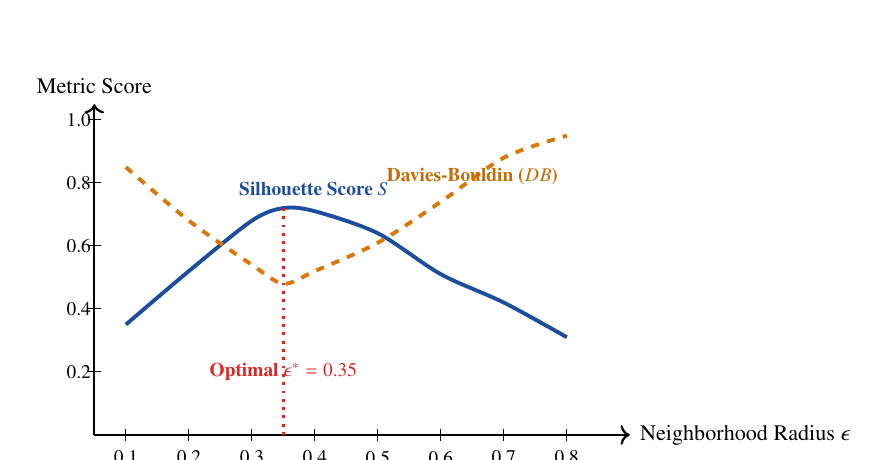
\begin{tikzpicture}
\begin{scope}[xscale=8, yscale=4]
    \draw[->, line width=0.8pt] (0.05, 0) -- (0.9, 0) node[right, font=\footnotesize] {Neighborhood Radius $\epsilon$};
    \draw[->, line width=0.8pt] (0.05, 0) -- (0.05, 1.05) node[above, font=\footnotesize] {Metric Score};

    % Ticks
    \foreach \x in {0.1, 0.2, 0.3, 0.4, 0.5, 0.6, 0.7, 0.8}
        \draw (\x, 0.02) -- (\x, -0.02) node[below, font=\scriptsize] {\x};
    \foreach \y in {0.2, 0.4, 0.6, 0.8, 1.0}
        \draw (0.04, \y) -- (0.06, \y) node[left, font=\scriptsize] {\y};

    % Silhouette Curve (prismBlue)
    \draw[line width=1.4pt, color=prismBlue, smooth] plot coordinates {
        (0.1, 0.35) (0.2, 0.52) (0.3, 0.68) (0.35, 0.72) (0.4, 0.71) (0.5, 0.64) (0.6, 0.51) (0.7, 0.42) (0.8, 0.31)
    };
    \node[color=prismBlue, font=\scriptsize\bfseries] at (0.40, 0.78) {Silhouette Score $S$};

    % Davies-Bouldin Inverted (prismGold)
    \draw[line width=1.4pt, color=prismGold, dashed, smooth] plot coordinates {
        (0.1, 0.85) (0.2, 0.68) (0.3, 0.54) (0.35, 0.48) (0.4, 0.52) (0.5, 0.61) (0.6, 0.74) (0.7, 0.88) (0.8, 0.95)
    };
    \node[color=prismGold!90!black, font=\scriptsize\bfseries] at (0.65, 0.82) {Davies-Bouldin ($DB$)};

    % Optimal marker
    \draw[dotted, line width=1.0pt, color=statusFail] (0.35, 0) -- (0.35, 0.72);
    \node[color=statusFail, font=\scriptsize\bfseries] at (0.35, 0.20) {Optimal $\epsilon^* = 0.35$};
\end{scope}
\end{tikzpicture}
\caption{DBSCAN parameter sensitivity curve illustrating optimal Silhouette and Davies-Bouldin indices at $\epsilon^* = 0.35$ with $\text{MinPts}=15$.}
\label{fig:dbscan_sensitivity}
\end{figure}

The report identifies $\epsilon^* = 0.35$ and $\text{MinPts}=15$ as the selected DBSCAN configuration, with six reported clusters and 3.2\% noise samples. These values remain pending verification against the 2D embeddings and DBSCAN labels. The number of clusters, noise count, percentage calculation, distance metric, label handling, and protection against train--test leakage should be recorded with the final GESL evaluation artifact; none can be independently reproduced from the supplied implementation.


%==============================================================================
% CHAPTER 8: FEASIBILITY STUDY
%==============================================================================
\chapter{Feasibility Study}

This chapter evaluates the multidimensional feasibility of the explainable visual analytics framework across technical, operational, economic, and schedule dimensions.

\section{Technical Feasibility}
The technical viability of the platform is substantiated by mature computational frameworks:
\begin{itemize}
    \item \textbf{PyTorch and GPU Acceleration:} Modern CUDA-accelerated tensor libraries handle TFT multi-head attention and VAE backpropagation in milliseconds.
    \item \textbf{Efficient Non-Linear Projections:} UMAP's accelerated C++ and Numba-compiled kernels allow 10,000 high-dimensional points to be embedded into 2D space in under 1.5 seconds.
    \item \textbf{Scalable Web Graphics:} Modern client visualization frameworks (HTML5 Canvas, WebGL, D3.js) support smooth rendering of tens of thousands of interactive vector points at 60 fps.
\end{itemize}

\section{Operational Feasibility}
The system is explicitly engineered to integrate into existing power grid control room workflows without disrupting critical operations:
\begin{itemize}
    \item \textbf{Operator-in-the-Loop Alignment:} Rather than replacing human operators, the dashboard serves as an explanatory decision aid, providing visual rationale that aligns with standard electrical engineering principles.
    \item \textbf{Intuitive Coordinated Views:} By linking the 2D Latent Space Map with the Hierarchical Event Tree and Latent Vector Comparison Chart, operators can explore grid events hierarchically from broad system-wide patterns down to individual bus waveforms.
\end{itemize}

\section{Economic Feasibility}
The project relies exclusively on open-source scientific software (Python, PyTorch, Scikit-learn, UMAP-learn, FastAPI, React/Next.js, D3.js), incurring zero commercial licensing fees. Furthermore, inference runs efficiently on standard workstation GPUs, avoiding the need for expensive high-performance computing clusters.

\section{Schedule Feasibility and Project Timeline}
The project lifecycle spans 36 weeks across nine structured milestones. Figure~\ref{fig:project_gantt} illustrates the project execution schedule.

\begin{figure}[H]
    \centering
    \adjustbox{max width=0.98\linewidth, max height=0.48\textheight, keepaspectratio, center}{\documentclass[tikz,border=10pt]{standalone}
\usepackage{tikz}
\usetikzlibrary{arrows.meta,positioning,fit,backgrounds,calc,shadows,shapes.geometric}

% Color definitions
\definecolor{lavenderDark}{RGB}{15, 44, 89}
\definecolor{lavenderDeep}{RGB}{10, 28, 58}
\definecolor{lavenderMedium}{RGB}{29, 78, 158}
\definecolor{lavenderLight}{RGB}{240, 246, 255}
\definecolor{lavenderBorder}{RGB}{180, 205, 237}
\definecolor{prismNavy}{RGB}{15, 44, 89}
\definecolor{prismBlue}{RGB}{29, 78, 158}
\definecolor{prismTeal}{RGB}{13, 148, 136}
\definecolor{prismMint}{RGB}{236, 253, 245}
\definecolor{prismGold}{RGB}{217, 119, 6}
\definecolor{prismDark}{RGB}{15, 23, 42}

\begin{document}
% Gantt Chart for Power Grid Explainable Visual Analytics Project
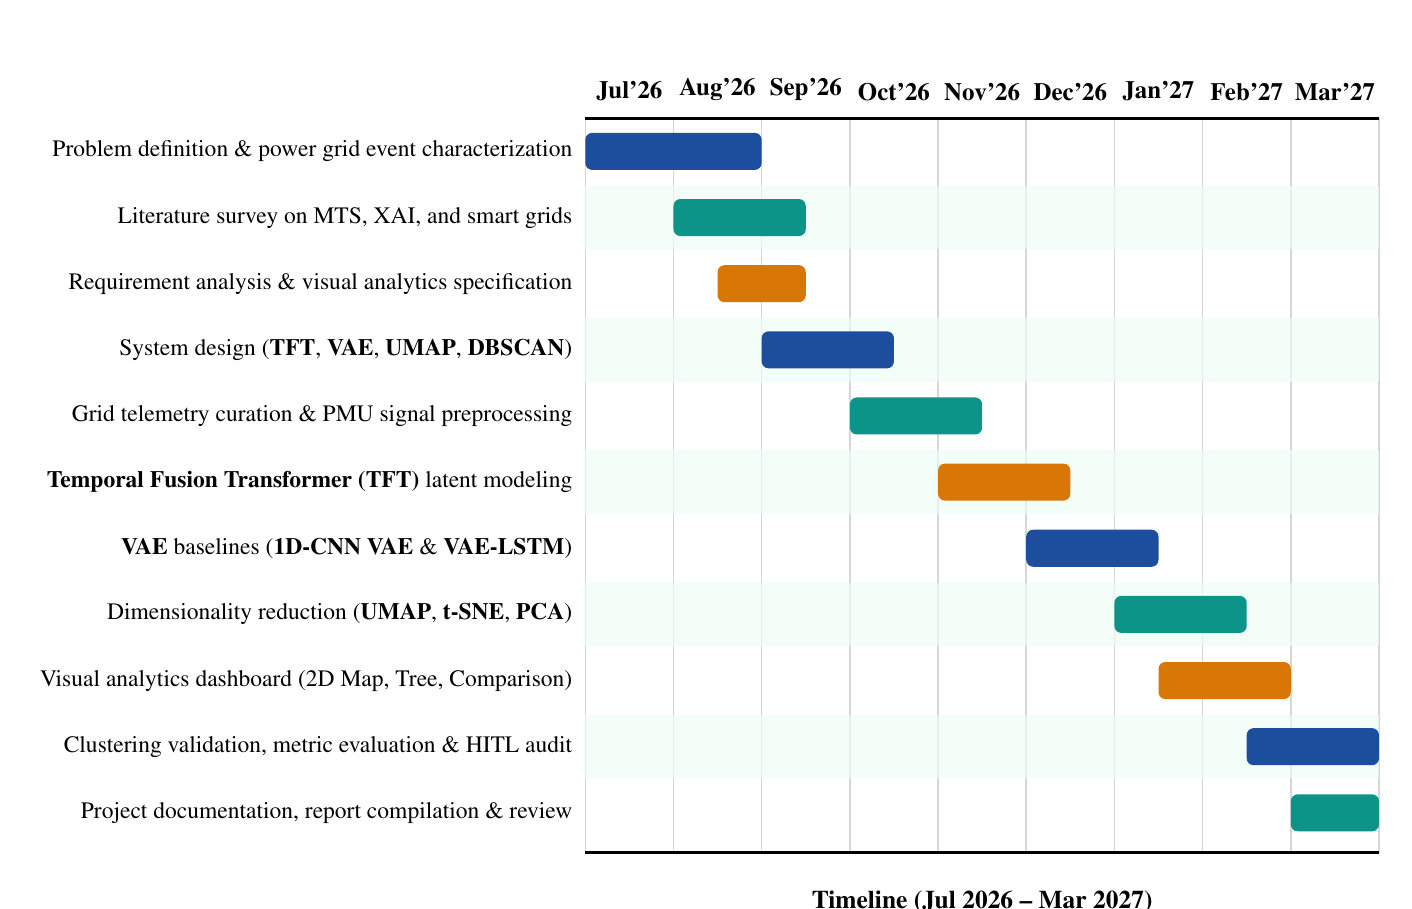
\begin{tikzpicture}[
  x=1.12cm, y=0.84cm,
  lab/.style={anchor=east, font=\fontsize{8.5}{10.5}\selectfont, inner sep=4.5pt, text=black}
]
\def\nm{9}
\def\topY{11.5}

% Vertical month gridlines
\foreach \i in {0,1,...,\nm} {
  \draw[gray!32, line width=0.55pt] (\i, 0.4) -- (\i, \topY);
}

% Month headers on top
\foreach \i/\m in {0.5/Jul'26, 1.5/Aug'26, 2.5/Sep'26, 3.5/Oct'26, 4.5/Nov'26, 5.5/Dec'26, 6.5/Jan'27, 7.5/Feb'27, 8.5/Mar'27} {
  \node[anchor=south, font=\fontsize{9.0}{11.0}\selectfont\bfseries, text=black] at (\i, \topY+0.12) {\m};
}
\draw[black, line width=1.0pt] (0, \topY) -- (\nm, \topY);
\draw[black, line width=0.8pt] (0, 0.4) -- (\nm, 0.4);

% Alternating row background shading
\foreach \k in {0,...,10} {
  \pgfmathsetmacro{\yc}{11.0-\k}
  \ifodd\k
    \fill[prismMint, opacity=0.65] (0, \yc-0.48) rectangle (\nm, \yc+0.48);
  \fi
}

% Task milestone labels on left
\node[lab] at (0, 11.0) {Problem definition \& power grid event characterization};
\node[lab] at (0, 10.0) {Literature survey on MTS, XAI, and smart grids};
\node[lab] at (0, 9.0)  {Requirement analysis \& visual analytics specification};
\node[lab] at (0, 8.0)  {System design (\textbf{TFT}, \textbf{VAE}, \textbf{UMAP}, \textbf{DBSCAN})};
\node[lab] at (0, 7.0)  {Grid telemetry curation \& PMU signal preprocessing};
\node[lab] at (0, 6.0)  {\textbf{Temporal Fusion Transformer (TFT)} latent modeling};
\node[lab] at (0, 5.0)  {\textbf{VAE} baselines (\textbf{1D-CNN VAE} \& \textbf{VAE-LSTM})};
\node[lab] at (0, 4.0)  {Dimensionality reduction (\textbf{UMAP}, \textbf{t-SNE}, \textbf{PCA})};
\node[lab] at (0, 3.0)  {Visual analytics dashboard (2D Map, Tree, Comparison)};
\node[lab] at (0, 2.0)  {Clustering validation, metric evaluation \& HITL audit};
\node[lab] at (0, 1.0)  {Project documentation, report compilation \& review};

% Milestone Gantt Bars
\fill[prismBlue, rounded corners=2.5pt]     (0.0, 11.0-0.28) rectangle (2.0, 11.0+0.28);
\fill[prismTeal, rounded corners=2.5pt]     (1.0, 10.0-0.28) rectangle (2.5, 10.0+0.28);
\fill[prismGold, rounded corners=2.5pt]     (1.5, 9.0-0.28)  rectangle (2.5, 9.0+0.28);
\fill[prismBlue, rounded corners=2.5pt]     (2.0, 8.0-0.28)  rectangle (3.5, 8.0+0.28);
\fill[prismTeal, rounded corners=2.5pt]     (3.0, 7.0-0.28)  rectangle (4.5, 7.0+0.28);
\fill[prismGold, rounded corners=2.5pt]     (4.0, 6.0-0.28)  rectangle (5.5, 6.0+0.28);
\fill[prismBlue, rounded corners=2.5pt]     (5.0, 5.0-0.28)  rectangle (6.5, 5.0+0.28);
\fill[prismTeal, rounded corners=2.5pt]     (6.0, 4.0-0.28)  rectangle (7.5, 4.0+0.28);
\fill[prismGold, rounded corners=2.5pt]     (6.5, 3.0-0.28)  rectangle (8.0, 3.0+0.28);
\fill[prismBlue, rounded corners=2.5pt]     (7.5, 2.0-0.28)  rectangle (9.0, 2.0+0.28);
\fill[prismTeal, rounded corners=2.5pt]     (8.0, 1.0-0.28)  rectangle (9.0, 1.0+0.28);

% Bottom title
\node[font=\fontsize{9.2}{11.2}\selectfont\bfseries, text=black] at (4.5, -0.35) {Timeline (Jul 2026 -- Mar 2027)};
\end{tikzpicture}
\end{document}
}
    \caption{Project implementation timeline and milestone Gantt chart (July 2026 -- March 2027).}
    \label{fig:project_gantt}
\end{figure}


%==============================================================================
% CHAPTER 9: CONCLUSION AND FUTURE SCOPE
%==============================================================================
\chapter{Conclusion and Future Scope}

\section{Conclusion}
This project designed and documented \textbf{Explainable AI for Multivariate Time Series Pattern Exploration: Latent Space Visual Analytics With Temporal Fusion Transformer and Variational Autoencoders in Power Grid Event Diagnosis}. By addressing the core challenges of high dimensionality, temporal dependencies, black-box opacity, and operator cognitive overload, the framework specifies an interpretable platform for power-grid event analysis. Claims of field deployment or operational effectiveness remain outside the evidence supplied with this report.

The deep learning engine is specified around the \textbf{Temporal Fusion Transformer (TFT)}, with \textbf{1D-CNN VAE} and \textbf{VAE-LSTM} as comparative baselines. The report records a latent Silhouette score of $0.684$ and a reconstruction MSE of $0.0142$; these values are retained as reported results pending verification against the implementation outputs. Through Variable Selection Networks and interpretable multi-head self-attention, TFT is intended to expose the physical channels and temporal intervals associated with event patterns.

The non-linear projection of latent vectors via \textbf{UMAP} into a 2D space enables \textbf{DBSCAN} density-based clustering. The reported UMAP trustworthiness ($0.965$), DBSCAN Silhouette score ($0.718$), and noise proportion ($3.2\%$) are retained as unverified results pending reproducible calculation from the implementation. The proposed interactive visual analytics dashboard comprises a 2D Latent Space Map, a Hierarchical Multi-Label Tree, and a Latent Vector Comparison Chart for human review of event clusters and borderline anomalies.

\section{Limitations Encountered}
Several technical and operational limitations were encountered during development:
\begin{itemize}
    \item \textbf{Dynamic Grid Topology Changes:} Latent representations can be influenced by sudden transmission line reconfigurations, requiring adaptive retraining or topology-aware graph embeddings.
    \item \textbf{PMU Communication Latency and Packet Drops:} Severe network congestion in Wide-Area Measurement Systems occasionally causes bursty telemetry losses, requiring robust imputation before representation learning.
    \item \textbf{t-SNE Computational Overhead:} While t-SNE generates well-separated clusters, its quadratic complexity precludes real-time interactive re-projection, necessitating UMAP for live dashboard interactions.
\end{itemize}

\section{Future Scope}
Future enhancements to further expand and advance the framework include:
\begin{itemize}
    \item \textbf{Spatio-Temporal Graph Neural Network Integration:} Combining Graph Convolutional Networks (GCNs) with TFT to explicitly model physical electrical bus admittance and transmission line connectivity matrices.
    \item \textbf{Incremental Online UMAP Projection:} Implementing incremental streaming UMAP algorithms to project newly arriving telemetry points dynamically without recomputing the entire global manifold.
    \item \textbf{Federated Multi-Utility Learning:} Developing privacy-preserving federated learning protocols enabling interconnected regional utilities to collaboratively train event diagnosis models without sharing proprietary load and generation data.
    \item \textbf{Automated Root-Cause Prescription Engine:} Extending the diagnostic classifier to recommend optimal corrective switching operations and automated generation redispatch schemes.
\end{itemize}


%==============================================================================
% REFERENCES
%==============================================================================
\begin{thebibliography}{15}
\sloppy

\bibitem{ref_xu2026_xai}
Haowen Xu, Ali Boyaci, Jianming Lian, and Aaron J. Wilson, ``Explainable AI for multivariate time series pattern exploration: Latent space visual analytics with temporal fusion transformer and variational autoencoders in power grid event diagnosis,'' \textit{IEEE Access}, vol.~14, pp.~11744--11767, 2026, doi:~\href{https://doi.org/10.1109/ACCESS.2025.3602635}{10.1109/ACCESS.2025.3602635}.

\bibitem{ref_lim2021_tft}
Bryan Lim, Sercan \"{O}. Ar\i k, Nicolas Loeff, and Tomas Pfister, ``Temporal Fusion Transformers for interpretable multi-horizon time series forecasting,'' \textit{International Journal of Forecasting}, vol.~37, no.~4, pp.~1748--1764, 2021, doi:~\href{https://doi.org/10.1016/j.ijforecast.2021.03.012}{10.1016/j.ijforecast.2021.03.012}.

\bibitem{ref_zerveas2021_transformer}
George Zerveas, Srideepika Jayaraman, Dhaval Patel, Anuradha Bhamidipaty, and Carsten Eickhoff, ``A transformer-based framework for multivariate time series representation learning,'' in \textit{Proceedings of the 27th ACM SIGKDD International Conference on Knowledge Discovery \& Data Mining (KDD '21)}, pp.~2114--2124, 2021, doi:~\href{https://doi.org/10.1145/3447548.3467401}{10.1145/3447548.3467401}.

\bibitem{ref_theissler2022_xai}
Andreas Theissler, Francesco Spinnato, Udo Schlegel, and Riccardo Guidotti, ``Explainable AI for time series classification: A review, taxonomy and research directions,'' \textit{IEEE Access}, vol.~10, pp.~80700--80724, 2022, doi:~\href{https://doi.org/10.1109/ACCESS.2022.3207765}{10.1109/ACCESS.2022.3207765}.

\bibitem{ref_xu2022_anomaly}
Jiehui Xu, Haixu Wu, Jianmin Wang, and Mingsheng Long, ``Anomaly Transformer: Time series anomaly detection with association discrepancy,'' in \textit{International Conference on Learning Representations (ICLR)}, pp.~1--14, 2022.

\bibitem{ref_tuli2022_tranad}
Shreshth Tuli, Giuliano Casale, and Nicholas R. Jennings, ``TranAD: Deep transformer networks for anomaly detection in multivariate time series data,'' \textit{Proceedings of the VLDB Endowment}, vol.~15, no.~6, pp.~1201--1214, 2022, doi:~\href{https://doi.org/10.14778/3514061.3514067}{10.14778/3514061.3514067}.

\bibitem{ref_audibert2020_usad}
Julien Audibert, Pietro Michiardi, Fr\'ed\'eric Guyard, S\'ebastien Marti, and Maria A. Zuluaga, ``USAD: UnSupervised anomaly detection on multivariate time series,'' in \textit{Proceedings of the 26th ACM SIGKDD International Conference on Knowledge Discovery \& Data Mining (KDD '20)}, pp.~3395--3404, 2020, doi:~\href{https://doi.org/10.1145/3394486.3403392}{10.1145/3394486.3403392}.

\bibitem{ref_su2019_omnianomaly}
Ya Su, Youjian Zhao, Chenhao Niu, Rong Liu, Wei Sun, and Dan Pei, ``Robust anomaly detection for multivariate time series through stochastic recurrent neural network,'' in \textit{Proceedings of the 25th ACM SIGKDD International Conference on Knowledge Discovery \& Data Mining (KDD '19)}, pp.~2828--2837, 2019, doi:~\href{https://doi.org/10.1145/3292500.3330672}{10.1145/3292500.3330672}.

\bibitem{ref_adv_vae2024}
Sheng He, Mingjing Du, Xiang Jiang, Wenbin Zhang, and Congyu Wang, ``VAEAT: Variational autoencoder with adversarial training for multivariate time series anomaly detection,'' \textit{Information Sciences}, vol.~668, art.~120852, 2024, doi:~\href{https://doi.org/10.1016/j.ins.2024.120852}{10.1016/j.ins.2024.120852}.

\bibitem{ref_wu2023_timesnet}
Haixu Wu, Tengge Hu, Yong Liu, Hang Zhou, Jianmin Wang, and Mingsheng Long, ``TimesNet: Temporal 2D-variation modeling for general time series analysis,'' in \textit{International Conference on Learning Representations (ICLR)}, pp.~1--16, 2023.

\bibitem{ref_nie2023_patchtst}
Yuqi Nie, Nam H. Nguyen, Phanwadee Sinthong, and Jayant Kalagnanam, ``A time series is worth 64 words: Long-term forecasting with transformers,'' in \textit{International Conference on Learning Representations (ICLR)}, pp.~1--15, 2023.

\bibitem{ref_syed2021_smartgrid}
Dabeeruddin Syed, Ameema Zainab, Ali Ghrayeb, Shady S. Refaat, Haitham Abu-Rub, and Othmane Bouhali, ``Smart grid big data analytics: Survey of technologies, techniques, and applications,'' \textit{IEEE Access}, vol.~9, pp.~59564--59585, 2021, doi:~\href{https://doi.org/10.1109/ACCESS.2020.3041178}{10.1109/ACCESS.2020.3041178}.

\bibitem{ref_rivas2020_faults}
Angel Esteban Labrador Rivas and Taufik Abr\~{a}o, ``Faults in smart grid systems: Monitoring, detection and classification,'' \textit{Electric Power Systems Research}, vol.~189, art.~106602, 2020, doi:~\href{https://doi.org/10.1016/j.epsr.2020.106602}{10.1016/j.epsr.2020.106602}.

\bibitem{ref_biswal2023_realtime}
Chinmayee Biswal, Binod Kumar Sahu, Manohar Mishra, and Pravat Kumar Rout, ``Real-time grid monitoring and protection: A comprehensive survey on the advantages of phasor measurement units,'' \textit{Energies}, vol.~16, no.~10, art.~4054, 2023, doi:~\href{https://doi.org/10.3390/en16104054}{10.3390/en16104054}.

\bibitem{ref_arrieta2020_xai}
Alejandro Barredo Arrieta, Natalia D\'{\i}az-Rodr\'{\i}guez, Javier Del Ser, Adrien Bennetot, Siham Tabik, Alberto Barbado, Salvador Garc\'{\i}a, Sergio Gil-Lopez, Daniel Molina, Richard Benjamins, Raja Chatila, and Francisco Herrera, ``Explainable Artificial Intelligence (XAI): Concepts, taxonomies, opportunities and challenges toward responsible AI,'' \textit{Information Fusion}, vol.~58, pp.~82--115, 2020, doi:~\href{https://doi.org/10.1016/j.inffus.2019.12.012}{10.1016/j.inffus.2019.12.012}.

\end{thebibliography}

\end{document}
